% ------------------------------
%Exemplo de dissertação do INF-UFG com texto em portugues formatado com LaTeX
%-----------------------------------------------------------------
\documentclass[dissertacao]{inf-ufg}
%Pacotes para tabelas longas e alinhamento vertical
\usepackage{rotating}
\usepackage{longtable}
\usepackage{multirow}
\usepackage{graphicx}
%Resolvendo problemas de acentuação
%\usepackage[brazil]{babel}
%\usepackage[utf8]{inputenc}

% Opões da classe inf-ufg (ao usar mais de uma, separe por vírgulas)
%   [tese]         -> Tese de doutorado.
%   [dissertacao]  -> Dissertação de mestrado (padrão).
%   [monografia]   -> Monografia de especializção.
%   [relatorio]    -> Relatório final de graduação.
%   [abnt]         -> Usa o estilo "abnt-alf" de citação bibliográfica.
%   [nocolorlinks] -> Os links de navegação no texto ficam na cor preta.
%                     Use esta opção para gerar o arquivo para impresso
%                     da versão final do seu texto!!!

%----------INICIO DO DOCUMENTO %

\begin{document}

%----------AUTOR, TÍULO E DATA DE DEFESA %
\autor{Jailton Alkimin Louzada} % ()
\autorR{Louzada, Jailton A} % (}

\titulo{FreeTest 2.0: Uma Evolução do Método FreeTest para Melhoria do Processo de Teste de Software em Micro, Pequenas Empresa Brasileiras}

%\titulo{Método FreeTest 2.0: Um Arcabouço com Guia de Implantação e Evolução do Processo FreeTest em Micro, Pequenas Empresas }


%\subtitulo{}

\cidade{Goiânia} % Nome da cidade em foi desenvolvido o trabalho
\dia{01} %
\mes{07} % Data da apresenta�ão/defesa do trabalho
\ano{2017} % Formato numérico: \dia{01}, \mes{01} e \ano{2009}

%-------------------------------------------------------------- ORIENTADOR %
\orientador{Dr. Celso Gonçalves Camilo Junior}
\orientadorR{Camilo-Junior, Celso G}
% Use os comandos a seguir se for Orientadora e nao Orientador.
\orientadora{Dr. Celso Gonçalves Camilo Junior}%
\orientadoraR{Camilo-Junior, Celso G}%Ferreira, Deller J

%\coorientador{Dr. Auri Marcelo Rizzo Vincenzi}%Dr. Sérgio Teixeira de Carvalho
%\coorientadorR{Vicenzi, Auri M R}%Carvalho, Sérgio T

%\coorientador{Dr. Cássio Leonardo Rodrigues}%Dr. Sérgio Teixeira de Carvalho
%\coorientadorR{Rodrigues, Cassio L}%Carvalho, Sérgio T

% Use os comandos a seguir se for Co-orientadora e nao Coorientador.
%\coorientadora{\textless Nome da Co-orientadora\textgreater}
%\coorientadoraR{\textless Nome Reverso da Co-orientadora\textgreater}

%-------------------------------------------------- INSTITUIÇÃO E PROGRAMA %
\universidade{Universidade Federal de Goiás} % {Universidade Federal de Goiás}
\uni{UFG} % UFG
\unidade{Instituto de Informática}%Instituto de Informática
%\departamento{INSTITUTO DE INFORMÁTICA} %Unidades com mais de um depto.

\universidadeco{Universidade Federal de Goiás}%Universidade Federal de Goiás
\unico{UFG}%UFG
\unidadeco{Instituto de Informática}

\programa{Ciência da Computação}% Computação
\concentracao{Ciência da Computação}

%-------------------------------------------------- ELEMENTOS PRÈ-TEXTUAIS %
\capa    % Gera o modelo da capa externa do trabalho
\publica % Gera a autorização para publicação em formato eletrônico
\rosto   % Primeira folha interna do trabalho


\begin{aprovacao}

%\banca{Dr. Celso Gonçalves Camilo Junior}{Instituto de Informática -- UFG}
\banca{Dr. Auri Marcelo Rizzo Vincenzi}{Instituto de Informática -- UFG}
\banca{Dr. Cássio Leonardo Rodrigues}{Instituto de Informática -- UFG}
% Use o comando \profa se o membro da banca for do sexo feminino.
%\profa{Dra. Fátima de Lourdes dos Santos Nunes Marques}{Escola de Artes, Ciências e Humanidades -- USP}

\end{aprovacao}
\direitos{Bacharelado em Ciência da Computação pela Pontifícia Universidade Católica de Goiás, pós graduado no curso de MBA em Gerenciamento de Projetos e com mais de seis anos trabalhando com Qualidade de Software, exercendo papéis de liderança e trabalhando com automação de testes e DevOps.}
\begin{dedicatoria}
Dedico este trabalho à minha família, principalmente à minha mãe e pai, Maria Helieni da Silva Alkimin e Jailton Neves Louzada, por estar ao meu lado em todos os momentos.
\end{dedicatoria}
\begin{agradecimentos}
A Deus por essa conquista alcançada e por estar ao meu lado nesta longa caminhada. Foram muitas dificuldades enfrentadas durante todo esse percurso, mas todas elas foram superadas com a graça de Deus.

À minha família, em especial aos meus pais, Jailton Neves Louzada e minha mãe Maria Helieni da Silva Alkimin.

Ao meu orientador, Dr. Celso Camilo pela compreensão, supervisão e paciência. Por meio dos seus conselhos, estou aprendendo o caminho da pesquisa científica. Sei que o caminho é longo, mas tive uma base sólida por intermédio das suas orientações. Agradeço toda a dedicação oferecida a mim durante este período de mestrado.

Aos meus co-orientadores, Dr. Auri Vicenzi e Dr. Cássio Rodrigues, pela supervisão, orientação e parceria. Sei que ainda tenho muito a aprender com os ensinamentos de vocês. Portanto, também agradeço a dedicação oferecida a mim durante este período de mestrado.

À Fundação de Amparo à Pesquisa do Estado de Goiás (FAPEG) pelo auxílio financeiro, o qual ajudou na viabilidade da execução desta pesquisa.

Aos amigos e colaboradores, que ajudaram de forma direta na realização deste trabalho, Paulo Marcos, Rhelcris Salvino, André Lobo, Tiago Nogueira, Daniel Gomes, Weder Cabral e Márcio Lima.

\end{agradecimentos}



\epigrafe{\textit{Refactoring changes the program in small steps. If you make a mistake, it is easy to find the bug.}}
{Martin Fowler}
{Refactoring: Improving the Design of Existing Code}
\chaves{Processo de Teste de Software, DevOps, Métodos Ágeis, MPT.Br}

\begin{resumo} 

\textbf{Contexto:} O mercado de Tecnologia da Informação (T.I.) é crescente. Na era da informação, as economias mundiais vêm investindo cada vez mais no mercado de Serviços. Dentro deste cenário competitivo, o teste de software é um importante componente para elevação da qualidade do software desenvolvido no Brasil e sua competitividade mundial. Contudo, as Micro e Pequenas Empresas (MPEs) possuem recursos limitados para investimentos em processos, ferramentas e modelos de maturidade de teste de software em seus negócios. Diante disto, este trabalho tem como proposta principal produzir um aparato para melhoria do processo de teste de software para MPEs. \textbf{Objetivo:} Como objetivos principais, este estudo propôs uma versão mais atualizada do processo FreeTest, bem como instruções práticas de como implantar as atividades sugeridas no processo, tudo isso formatado em um novo processo e um guia de implantação respectivamente. \textbf{Metodologia:} Com o propósito de cumprir os objetivos almejado neste trabalho foram criados o processo FreeTest 2.0 como uma melhoria do processo do Método FreeTest, focado principalmente em técnicas Ágeis, DevOps e alinhado ao ecossistema das MPEs. E o FreeTest Wizard, que consiste em um guia de implantação que apoia a implantação do processo de forma didática, dinâmica e flexível. Outra contribuição deste trabalho foi a criação de ferramentas de apoio para disseminação deste conhecimento e gestão dos conteúdos, neste caso a criação de uma plataforma web, distribuída de forma gratuita e no formato "\textit{as a Service}". Por fim, os \textbf{resultados} e \textbf{conclusões} poderão ser vistos no capítulo final deste trabalho.

\end{resumo}
\keys{Software Testing Process Improvement, DevOps, Agile Frameworks, MPT.Br}

\begin{abstract}{FreeTest Framework - A Framework for Improvement of the Software Testing Process in midsized brazilian companies and startups}

The Information Technology market (T.I.) is growing. In the information age, world economies have been investing more and more in the services market. Within this competitive scenario, software testing is an important component for raising the quality of software developed in Brazil and its global competitiveness. However, Micro and Small Enterprises (MPEs) and startups have limited resources for investments in software testing maturity processes, tools and models in their business. In view of this, this work has as general proposal to produce an apparatus for improvement of software testing process for MPEs and startups. Within this apparatus, a generic and generic generic test process model was created, containing list of specific practices, maturity levels and list of supporting tools. To facilitate the deployment of the test process, a deployment guide was created to assist MPEs and startups in deploying the test process. This deployment guide will act as a deployment wizard (online), which, based on a series of questions, will help the company to implement the process in the best possible way, from the point of view of its Level of maturity and support tools that the process supports.

The defined testing process has been redesigned based on the old FreeTest Method testing process, in this case now, containing process areas, specific activities and tools that are aligned to the ecosystem of MSEs and startups. The focus of this new process was to insert activities that could be automated, since they were well-accepted activities by the MSEs, since in their context, the technical team is usually formed by a large majority of developers and a small portion by testers, facilitating So the entry of automated mechanisms to carry out activities focusing on the quality of the code. Finally, the implementation guide and the process framework have been made available on a web platform and will be used to facilitate the implementation and maintenance of the process.

\end{abstract}


\tabelas[figtab]
%Opçôs:
%nada [] -> Gera apenas o sumário
%fig     -> Gera o sumário e a lista de figuras
%tab     -> Sumário e lista de tabelas
%alg     -> Sumário e lista de algoritmos
%cod     -> Sumário e lista de códigos de programas
%
% Pode-se usar qualquer combinação dessas opções.
% Por exemplo:
%  figtab       -> Sumário e listas de figuras e tabelas
%  figtabcod    -> Sumário e listas de figuras, tabelas e
%                  códigos de programas
%  figtabalg    -> Sumário e listas de figuras, tabelas e algoritmos
%  figtabalgcod -> Sumário e listas de figuras, tabelas, algoritmos e
%                  códigos de programas
%\input{./pre/pre_termos}
%--------------------------------------------------------------- CAPÍTULOS %
\chapter{Introdução}
\label{cap:intro}

% Este capítulo introduz os passos iniciais realizados nesta pesquisa. Uma visão geral e estruturada desse trabalho é apresentado e por fim um direcionamento aos demais tópicos deste trabalho.

% \section{Problema e Justificativa}
% \label{cap:problema}

% No contexto mundial, as Micro Pequenas Empresas (MPEs) representam cerca de 99,2\% das empresas do mundo \cite{Laporte2010, Ramachandram2008}. 

No Brasil o crescimento em investimentos em Tecnologia da Informação (T.I.) tem sido grande, só no ano de 2013 foi constatado um aumento de 15,4\% em relação ao ano anterior \cite{SilvaDias2015}. Segundo dados da consultoria IDC \footnote{http://br.idclatin.com/} (\textit{International Data Corporation}), o mercado brasileiro de Tecnologia da Informação terá um crescimento na ordem de 2,6\% no ano de 2016. Apesar dos números de 2015 não terem sido efetivados, a consultoria acredita que haverá uma expansão nos investimentos em T.I. no Brasil. Sendo assim, o setor deverá manter um faturamento superior aos US\$ 60 bilhões, “mesmo diante de um cenário econômico adverso”, afirma a empresa \cite{FelipeDreher2016}. De acordo com esses resultados, o Brasil se manteve em 1º lugar do ranking de investimento no setor de T.I. na América Latina, com 45\% dos investimentos, somando US\$ 59,9 bilhões \cite{FelipeDreher2016}.

No ano de 2015 o Brasil possuía aproximadamente 13.950 empresas dedicadas ao desenvolvimento, produção, distribuição de software e de prestação de serviços, sendo aproximadamente 58\% das empresas de desenvolvimento e produção de software ou prestação de serviço \cite{abranet2016}. No cenário nacional a região sudoeste lidera o mercado brasileiro de T.I. com 60,44\% enquanto que as regiões, Sul (13,95\%), Norte (4,24\%), Nordeste (10,72\%) e Centro-Oeste (10,64\%) ocupam uma parcela não muito significativa (vide tabela \ref{tab:1.1}).

\begin{table}[H]
\centering
\caption{Distribuição regional do mercado brasileiro de T.I. \cite{abes-software2016}}.
\label{tab:1.1}
\begin{tabular}{|c|c|c|c|c|}
\hline
\textbf{Região}       & \textbf{Hardware} & \textbf{Software} & \textbf{Serviços} & \textbf{Total} 
    \\ \hline
\textbf{Norte}        & 5,22\%            & 3,06\%            & 2,94\%            & 4,24\%         
    \\ \hline
\textbf{Nordeste}     & 12,88\%           & 8,67\%            & 7,43\%            & 10,72\%        
    \\ \hline
\textbf{Sul}          & 14,6\%            & 13,18\%           & 13,11\%           & 13,95\%          
    \\ \hline
\textbf{Centro-Oeste} & 9,88\%            & 11,38\%           & 11,8\%            & 10,64\%        
    \\ \hline
\textbf{Sudeste}      & 57,42\%           & 63,71\%           & 64,72\%           & 60,44\%        
    \\ \hline
\end{tabular}
\end{table}

No estudo intitulado “Mercado Brasileiro de Software e Serviços” \cite{abes-software2016}, cerca de 94\% das empresas de T.I. são classificadas como Micro e Pequenas Empresas. No entanto grande parte das MPEs não aplicam investimentos em qualidade, especificamente em processos de desenvolvimento, teste de software, ferramentas, capacitação técnica e outros. Por isso, segundo a Softex \cite{GuiaMPTbr} cerca de 40\% de novos produtos de software disponibilizados no mercado falham.

Com o intuito de atender as necessidades em termos de qualidade do desenvolvimento de software das MPEs, o FreeTest 1.0 \cite{Camilo-junior2012} foi criado, e consiste em um conjunto de processos e ferramentas com a intenção de viabilizar o teste de software em MPEs de forma fácil e com baixo custo. Esse método foi pensado de maneira a estabelecer soluções de fácil aplicação, que sejam integrados às ferramentas de desenvolvimento da Organização. O FreeTest 1.0 foi desenvolvido por um grupo de pesquisadores do Instituto de Informática da Universidade Federal de Goiás (INF/UFG) \cite{Camilo-junior2012} em parceria com um consórcio de MPEs do estado de Goiás e com recursos de fomento à inovação do programa PAPPE-INTEGRAÇÃO, da FAPEG/FINEP. Todavia, com o crescimento emergente do mercado de T.I. e necessidade de atender as demandas do mercado de maneira mais ágil e com qualidade, tendo em vista as características das MPEs faz-se necessário algumas melhorias no FreeTest 1.0, principalmente no que diz respeito à práticas automatizadas que geram resultados mais rápidos e com baixo custo, quando implantadas corretamente. Outra questão observada é a necessidade de práticas especificas que ajudem as organizações a resolverem problemas corriqueiros na área de desenvolvimento e qualidade do software, e que concentre na preservação da entrega de software com valor e com abordagens baseadas em princípios \textit{lean} \footnote{https://www.agilealliance.org/agile101/12-principles-behind-the-agile-manifesto/} e ágil.

Uma característica no contexto das empresas de T.I. é que durante vários anos a indústria desenvolveu software de forma prescritiva (sequencial e linear), ou seja, utilizou-se de práticas de desenvolvimento de software similarmente a outras atividades de áreas como a engenharia. Na literatura pode encontrar alguns estudos sobre modelos prescritivos, como em Pressman \cite{PRESSMAN2011}, que menciona modelos como: Cascata, incrementais, evolucionários e espirais. Estes modelos atuam com o sequenciamento de fases e a prescrição das atividades, tarefas, produtos, mecanismos de garantia de qualidade e produto para cada projeto. 

Durante muito tempo os modelos prescritivos atenderam às necessidades de negócio das empresas de T.I. Contudo, hoje em dia, com necessidades de negócios das empresas mudando constantemente, implicando alterações constantes de requisitos esses modelos têm se tornado incompatíveis com o ecossistema das organizações de T.I. Diante dessas dificuldades dos modelos prescritivos atenderem as constantes mudanças foram propostos métodos mais ágeis, que têm como principal objetivo que as Organizações de T.I. respondessem de forma dinâmica as constantes mudanças do negócio. Com isso, equipes de desenvolvimento e requisitos se tornaram mais eficientes e realizam entregas de software mais rápidas em um período de tempo menor. Contudo, isso acarretou uma sobrecarga para a equipe de operação/suporte, pois com a geração de \textit{builds} muito maior que antes e a necessidade de por em produção os softwares desenvolvidos aumentou, assim surgiu outro problema não contemplado por esses métodos \cite{BRAGA2015}: Como realizar entregas constantes de software de forma efetiva, eficaz e que responda rapidamente às constantes mudanças dos requisitos?

Para resolver esse novo gargalo entre o desenvolvimento do software e sua entrega surgiu o movimento DevOps \cite{Debois2008}, com o objetivo de romper as barreiras tradicionais entre as equipes de desenvolvimento e operação, promovendo o uso de colaboração constante entre os times e com o foco no negócio/requisitos e suas mudanças constantes. Desta maneira, com a ajuda de práticas DevOps, o código produzido no desenvolvimento será implantado pela equipe de operação de forma rápida e previsível, fornecendo um fluxo de trabalho com entregas contínuas de software. Com isso é possível, por exemplo, realizar entregas diárias com o intuído de aumentar a confiabilidade, estabilidade, resistência e segurança do software entregue.

Considerando a importância das MPEs no desenvolvimento de software no mercado nacional e global, a importância de métodos mais ágeis de desenvolvimento e teste de software, este trabalho propõe; um processo de teste mais ágil, denominado FreeTest 2.0, evoluído a partir do Método FreeTest 1.0 \cite{Camilo-junior2012} e MPT.Br \cite{GuiaMPTbr}, que incluí práticas DevOps e Métodos Ágeis; e uma ferramenta web para apoiar a gestão e implantação do processo de teste proposto.

\section{Relevância da Pesquisa}

O mercado de T.I. é cada vez mais emergente. Especificamente no contextos das MPEs de T.I, há uma carência muito grande em estudos na acadêmia no sentido de ajudar as organizações a resolverem problemas corriqueiros na área de desenvolvimento e qualidade do software. Com o propósito de atender às particularidades das MPEs, algumas iniciativas, inclusive nacionais de modelos de maturidade e processos de teste além de normas internacionais vêm sendo propostas, tais como, Método Freetest 1.0 \cite{Camilo-junior2012}, a Melhoria do Processo de Teste Brasileiro (MPT.Br) \cite{GuiaMPTbr} e a \textit{International Organization for Standardization} (ISO)/ \textit{International Electrotechnical Commission} (IEC)/ \textit{Institute of Electrical and Electronic Engineers} (IEEE) 29119-2 \cite{Standard2013}. No entanto, essas propostas de melhoria de processo não contemplam as novas necessidades das MPEs de T.I., como, por exemplo, processos mais dinâmicos, menos prescritivos, ou seja, mais ágeis. 

% Outro fator que corroborou essa pesquisa é que não foram encontradas pesquisas que que auxiliem às Organizações de maneira mais ampla e prática, ofertando um processo, sugerindo ferramentas e disponibilizando um guia de apoio para implantação do processo de teste de forma fácil, \textit{as-a-Service}\footnote{http://searchcloudcomputing.techtarget.com/definition/XaaS-anything-as-a-service} (Do inglês, como serviço) e gratuita.

\section{Objetivos da Pesquisa}
\label{cap:objetivos}

Este trabalho objetiva a melhoria do processo de teste de software do Método FreeTest 1.0 \cite{Camilo-junior2012}, de agora em diante denominado FreeTest 2.0, e um guia de implantação para o Método FreeTest 2.0.

% Através do enfoque em práticas ágeis, técnicas DevOps, um processo de teste genérico e uma plataforma para modelagem dos processos da Organização. No que diz respeito ao processo uma \textit{wiki}, contendo o processo com suas Áreas de Processo e Práticas Especificas e lista de ferramentas de apoio será disponibilizada. 

% Por fim, como maior contribuição desse trabalho será disponibilizado para a comunidade um guia de implantação didático, chamado FreeTest Wizard para que Organizações que desejem implantar o processo, possam realizar a implantação passo-a-passo de forma intuitiva, rápida e com baixo custo. 

Em síntese esse trabalho tem como objetivos específicos:

\begin{itemize}
    \item Processo de Teste de Software, chamado \textbf{FreeTest 2.0}, voltado para MPEs com enfoque em práticas ágeis e DevOps;
    % \item Ferramenta Web contendo um processo de teste genérico e modelagem deste processo, bem como uma ferramenta que permitirá à organização modelar seus demais processos;
    \item \textbf{FreeTest Wizard}. Consistirá em um guia de implantação, no formato \textit{“wizard”} que através de uma interação com o usuário auxiliará na implantação do processo de teste na organização. 
    % \item Através do Guia de Implantação e do Arcabouço do processo será possível disponibilizar como serviço (\textit{As-a-Service}) uma plataforma/ferramenta \textit{online} para criação/manutenção dos processos de teste das organizações.
\end{itemize}

% \section{Procedimentos Metodológicos}
% \label{sec:procedimentos}

% Como procedimentos metodológicos para se alcançar os resultados desta pesquisa foram realizadas revisões na literatura sobre o estado da prática de \textit{frameworks} de teste, processos de uso específicos em teste de software, métodos ágeis e DevOps no contexto da indústria e com aplicação prática. Sendo que para guiar os resultados das buscas, alguns instrumentos de revisão sistemática foram utilizados, apesar deste estudo não realizar uma revisão sistemática em si, a ajuda de algumas etapas desta técnica foram muito úteis, principalmente para nortear os resultados e combiná-los com o conhecimento empírico dos autores. Abaixo a lista de perguntas que nortearam as buscas por literaturas utilizadas neste trabalho:

% \begin{itemize}
%     \item Q01 - Existem na literatura trabalhos de revisões sistemáticas sobre processos de teste de software?
%     \item Q02 - Quais são os processos, métodos e \textit{frameworks} de testes de software desenvolvidos nos últimos cinco anos?
%     \item Q03 - Quais trabalhos estão aplicando DevOps e Métodos Ágeis em processo de teste?
% \end{itemize}

\section{Organização do Trabalho}
\label{cap:estrutura}

Além deste capítulo, que apresenta a definição do problema e a justificativa, a relevância da pesquisa e os objetivos, o presente trabalho está organizado da seguinte forma:

\begin{itemize}
    \item Com intuito de realizar a fundamentação desta pesquisa, o \textbf{Capítulo     \ref{sec:referencialteorico}} traz o referencial teórico com os conceitos de Teste de Software, DevOps, Métodos Ágeis, Processos de Teste, Modelos de Processo e trabalhos relacionados. Buscando a originalidade e relevância desta pesquisa este capítulo apresenta também uma revisão da literatura sobre processos de teste especifico e ferramentas de amparo à implantação de processos.
    \item Com o propósito de alcançar os objetivos desta pesquisa, no \textbf{Capítulo \ref{sec:construcaoframeworkprocesso}} é apresentado a construção do Processo FreeTest 2.0.
    \item Com o propósito também de alcançar os objetivos desta pesquisa, no \textbf{Capítulo \ref{sec:construcaoguiaimplantacao}} é apresentado a construção do Guia de Implantação do Processo.
    \item Outro resultado deste trabalho é exposto no \textbf{Capítulo \ref{sec:ferramentas}} que apresenta detalhadamente as ferramentas de apoio criadas durante esta pesquisa. Neste caso a plataforma web que abrange o Gestor de Processos para o FreeTest 2.0 e o FreeTest Wizard para o Guia de Implantação.
    \item No \textbf{Capítulo \ref{sec:conclusaoetrabalhosfuturos}} são realizadas as conclusões finais deste trabalho e as sugestões para trabalhos futuros.
\end{itemize}
\chapter{Referencial Teórico}
\label{sec:referencialteorico}

Este capítulo apresenta o referencial teórico sobre teste de software, processos de teste mais consolidados e algumas técnicas reconhecidas e utilizadas amplamente pela comunidade acadêmica e indústria.

Serão apresentados na seção \ref{sec:processotestedesoftware} os conceito sobre os processos de teste prescritivos e ágeis, tomando como referencial alguns processos mais conhecidos na acadêmia.

Na seção \ref{sec:devops} apresentados conceitos e uma visão prática sobre DevOps e sua importância.

A subseção \ref{sec:revisaoliteraturacap2} é apresentado uma revisão da literatura, utilizando algumas técnicas de revisão sistemática.

Na seção \ref{sec:planejamentodapesquisa} é explanado toda a sistemática para realização da pesquisa do referencial teórico utilizado para este trabalho, bem como, strings de busca utilizadas, fontes de pesquisa e critérios de seleção dos estudos.

A subseção \ref{sec:identificacaodosestudos} mostra os passos necessários para a identificação dos estudos. Enquanto que na seção \ref{sec:selecaodosestudos} os estudos selecionados são exibidos, após sofrer os critérios de inclusão e exclusão.

Através dos resultados obtidos nas pesquisas, os trabalhos selecionados são discutidos na seção \ref{sec:discussoes}. Por fim, a conclusão deste capítulo é exposta na seção \ref{sec:conclusoescap2}.


\section{Processo de Teste software}
\label{sec:processotestedesoftware}

É uma atividade sistemática aplicada durante a integração da estrutura do programa visando a descobrir erros associados as interfaces entre os módulos. De acordo com Myers \cite{myers2004}, o principal objetivo do teste de software é revelar a presença de erros no produto. Atividade bastante efetiva em evidenciar a presença de defeitos de software. Sendo assim, um teste bem sucedido é aquele que consegue determinar casos de teste para os quais o programa em teste falhe.

O processo de teste de software consiste em uma analise dinâmica do produto, identificando e eliminando erros que persistem. O teste de produtos de software envolve basicamente quatro etapas:

\begin{itemize}
    \item Planejamento de testes;
    \item Projeto de casos de teste;
    \item Execução e avaliação dos resultados dos testes;
    \item Relato de erros.
\end{itemize}

\subsection{Processos Prescritivos}

Na história, o os softwares foram desenvolvidos de forma prescritiva, utilizando-se de práticas de desenvolvimento de software semelhantes a outras atividades de áreas como a engenharia civil \cite{BRAGA2015}. Nestas áreas inicialmente é definido um conjunto específico de ações, atividades e tarefas definidas em fases de forma sequencial e linear. Alguns modelos prescritivos são citados em Pressman \cite{PRESSMAN2011} como o modelo em cascata (Figura \ref{fig:figure21}) e modelos incrementais (Figura \ref{fig:figure22}), onde as características principais são o sequenciamento das fases. As fases de um modelo tradicional costumam seguir a sequencia composta por definição de requisitos, projeto do software, implementação, testes, integração, operação e manutenção.

\begin{figure}[!ht]
\centering
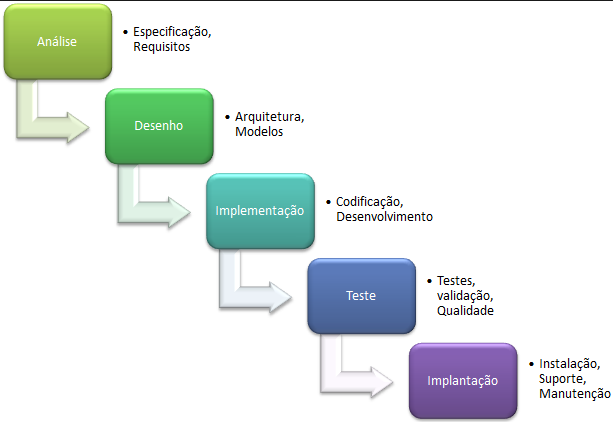
\includegraphics[width=.75\textwidth]{fig/figura21.png}
\caption{Exemplo de Modelo de Processo Cascata. (Fonte: Internet)}
\label{fig:figure21}
\end{figure}


\begin{figure}[!ht]
\centering
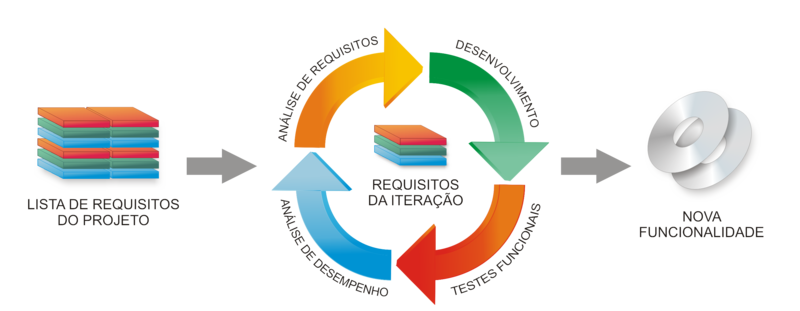
\includegraphics[width=.75\textwidth]{fig/figura22.png}
\caption{Exemplo de Modelo de Processo incremental. (Fonte: Internet)}
\label{fig:figure22}
\end{figure}

Em modelos tradicionais de desenvolvimento de software, a equipe de qualidade trabalham em de forma independente e muitas vezes em salas diferentes, aguardando a finalização do trabalho dos desenvolvedores para começarem a iniciar a etapa de testes (verificação e validação) no software. 
Após a realização dos testes, correção de possíveis \textit{bugs} e retestes, o software estará prestes a ser distribuído para os clientes, ou seja, estará em produção. Atividade essa desempenhada pela equipe de suporte, migração ou \textit{sysadmin} da organização.

Segundo Huttermann \cite{huttermann2012}, este modelo de trabalho com equipes separados gera barreiras como a ausência de uma padronização, pois, “\textit{uma vez que cada time desenvolve idioma próprio trabalhando em seus problemas individualmente e não em prol de um único objetivo.}” 

\subsection{Processo Ágil}

Com a necessidade cada vez maior do mercado consumidor de software, existe uma necessidade muito grande do mercado para que as empresas criem valor para os seus clientes através de software. Portando a entrega do software se tornou um dos grandes desafios das organizações, com a premissa de que software pronto é software em produção. Diante disso, e da necessidade de entrega de valor aos seus clientes os \textit{gaps} entre requisito, codificação, teste e entregam precisaram ser reduzidos. As organizações descobriram que os modelos tradicionais de desenvolvimento de software e de entrega não são suficientes. Os processos manuais são propensos a erros, quebras, desperdício e atraso de resposta às necessidades de negócios \cite{BRAGA2015}. Com a automatização de tarefas, criação de equipes multitarefas, e forma de trabalho holística as organizações podem focar no que realmente é importante: A entrega de valor aos seus clientes. Ao contrário de um modelo de desenvolvimento burocrático, sequencial e orientado à contratos as organizações tem se atentado que é importante a automatização de tarefas e entrega (mesmo que parciais) de valor aos seus clientes.

As metodologias tradicionais traziam um desenvolvimento de software pautado em estágios sequenciais e lineares, e são atualmente denominadas metodologias pesadas ou orientadas a documentação, porque cada o término de cada etapa é associado a uma documentação padrão que deve ser aprovada e assim poderá ser iniciada uma nova etapa \cite{ROYCE1970}. Nestas metodologias toda a responsabilidade por identificar \textit{bugs} é da equipe de qualidade, e o software não chega até o cliente até que a equipe de qualidade valide, a equipe de administração de redes, baco de dados e sistemas prepare o ambiente e por fim, a equipe de operação prepare o sistema para produção. Consequentemente os erros são encontrados tardiamente, os requisitos poderão não mais satisfazer as necessidades do negócio, e mais caro ficará o para corrigir e desenvolver novas soluções \cite{PRESSMAN2011}.

Inspirado em resolver as dificuldade proporcionada pela metodologia tradicional de desenvolvimento de software nasceu, na década de 90, o movimento ágil, que teve como principal objetivo que a equipe de desenvolvimento de software respondesse de forma mais dinâmica às constantes mudanças do negócio. Foi então estabelecido o Manifesto Ágil \cite{Beck2001}, visando priorizar os \textit{indivíduos, software executável, colaboração com o cliente, respostas rápidas a mudanças}, interações a processos e ferramentas e negociação de contratos.

No contexto das metologias ágeis várias possíveis e prováveis divergências entre o negócio e o produto se tornaram mais fáceis de serem resolvidas através de técnicas de aproximação do cliente à equipe de desenvolvimento, proporcionando integração contínua, reuniões diárias e times pequenos porém multifuncionais. Após a fase de aceitação e adaptação das empresas às metodologias ágeis de desenvolvimento, os desenvolvedores, testadores e demais membros da equipe do projeto se agruparam em prol do objetivo de desenvolver software ágil que respondessem às necessidades do negócio. Porém, ainda nesse novo contexto, a equipe de operação continuou isolada trabalhando como um time a parte, recebendo os \textit{builds}, integrando-os e os colocando em produção. E elas estão sendo cada vez mais aceitas pielas organizações, pois estas vem descobrindo que os modelos tradicionais de desenvolvimento de software e de entrega não são suficientes. Os processos manuais são propensos a erros, quebras, desperdício e atraso de resposta às necessidades de negócios \cite{WOOTTON2013}. Como visto na figura \ref{fig:figure23} em um processo Ágil a organização está orientada à entrega do produto, neste caso as entregas parciais são realizadas em curtos prazos de tempo para que os clientes possam validar os resultados e o desenvolvimento do software esteja alinhado ao negócio.


\begin{figure}[H]
\centering
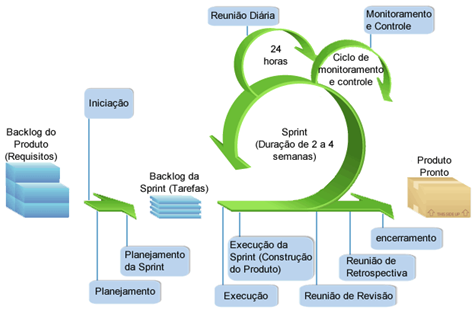
\includegraphics[width=.75\textwidth]{fig/figura23.png}
\caption{Exemplo de Modelo de Processo Ágil. (Fonte: Internet)}
\label{fig:figure23}
\end{figure}

\section{DevOps}
\label{sec:devops}

O Termo DevOps teve sua origem em 2008 quando \textit{Patrick Debois} publicou um artigo intitulado “\textit{Agile and Operations Infrastrucuture: How Infra-gile Are You?}” \cite{Debois2008}. Onde demonstrava que a infraestrutura poderia também responder de forma ágil à mudanças de negócios, se adaptando e respondendo constantemente. Neste ano, durante uma conferência sobre práticas ágeis houve a apresentação “\textit{Agile Infrastructure}” de Debois e \textit{Andrew Shafer}, onde também foi criada a lista \textit{agile-sysadmin} na Europa focada na discussão de metodologias ágeis na infraestrutura. A partir desta lista, vários estudos e conferências surgiram, popularizando o termo. Até que em 2009 hove a conferência \textit{Velocity da O’Reilly} onde foi apresentado o trabalho “\textit{10+ Deploys Per Day: Dev and Ops Cooperation at Flickr}” por  John Allspaw e Paul Hammond demonstrando o estudo de caso sobre a implantação em uma empresa onde havia a prática da colaboração entre as equipes de desenvolvimento e operação em atendimento à dinâmica do mercado \cite{ALLSPAW2009}. A partir deste evento surgiu a ideia de criar um novo evento, o DevOpsDays, realizados em diversos países, a partir de iniciativas locais, disseminando essa nova cultura.

Atualmente o termo DevOps é muito amplo, envolve inúmeras atividades e aspectos, como a automação, medição e o compartilhamento de conhecimentos \cite{huttermann2012} e pode se referir a qualquer prática que inova a interação entre desenvolvimento e operações. É uma abordagem baseada em princípios \textit{Lean} e Ágil \cite{BRAGA2015}. De tal maneira, que permite a Organização focar esforços no produto/cliente de maneira rápida, eficiente, de maneira contínua e com \textit{feedbacks} mais rápidos, onde, toda a equipe de desenvolvimento, qualidade e operação trabalha de forma colaborativa e simbiótica. Na figura \ref{fig:figure24} é possível entender o funcionamento de um modelo de processo que utiliza DevOps, no qual uma quantidade grande de atividades corriqueiras são criadas e a integração entre operação, teste e desenvolvimento ocorre o tempo todo de forma automatizada.

\begin{figure}[H]
\centering
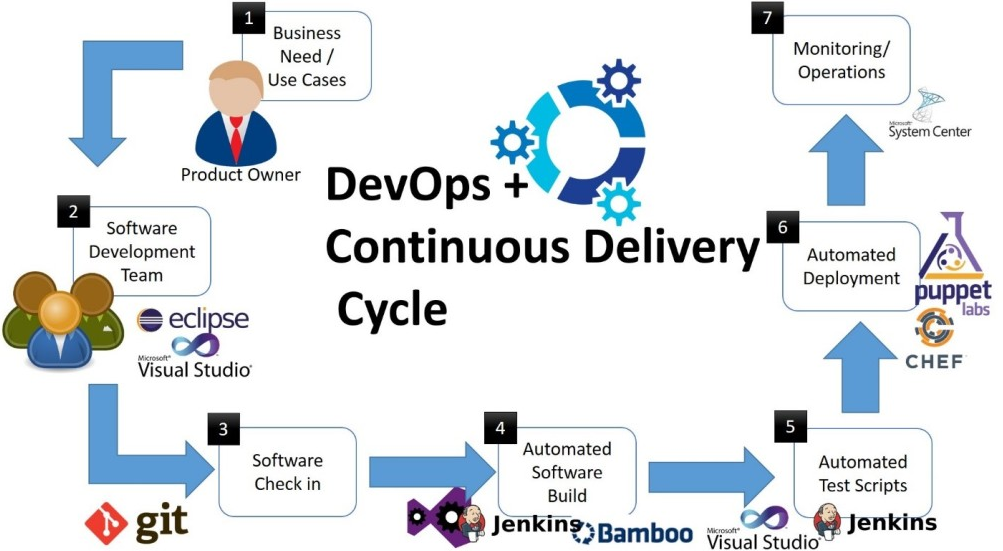
\includegraphics[width=.75\textwidth]{fig/figura24.png}
\caption{Exemplo de Modelo de Processo que utiliza DevOps. (Fonte: Internet)}
\label{fig:figure24}
\end{figure}

Em resumo, segundo Braga \cite{BRAGA2015} o DevOps é um movimento cultural, focado na colaboração e do compartilhamento de conhecimentos entre as equipes. A Organização pode possuir processos e ferramentas automatizadas eficientes, contudo se torna inútil senão utilizada corretamente. 
Por fim, construir uma cultura pautada nos objetivos da Organização ao invés dos objetivos da equipe separada é o que o DevOps preconiza.

\section{Revisão da Literatura}
\label{sec:revisaoliteraturacap2}

Esta sessão apresenta uma revisão da literatura sobre quais são os processos, métodos, e \textit{frameworks} de teste existentes no ponto de vista acadêmico e da indústria. Esta pesquisa incide sobre os artigos científicos publicados nos últimos cinco anos, a partir de janeiro de 2010 a dezembro de 2015.

Elenca-se que apesar de se utilizar algumas ferramentas da revisão sistemática, este estudo não visa realizar uma revisão sistemática, e sim, recuperar resultados efetivos das máquinas de busca mais conhecidas, aplicando expressões e filtros de datas e idiomas no qual as pesquisas foram escritas. 

O principal objetivo desta revisão da literatura foi buscar pesquisas relacionadas à processos de uso especifico para o Teste de Software, uso de DevOps e Métodos Ágeis. Preferencialmente trabalhos com estudo de caso e aplicações na indústria foram selecionados, com o intuito de enriquecer mais ainda essa pesquisa. Para nortear a pesquisa, foram concebidas as seguintes questões:

\begin{itemize}
\item Q01 - Existem na literatura trabalhos de revisões sistemáticas sobre processos de teste de software?   
\item Q02 - Quais são os processos, métodos e \textit{frameworks} de testes de software desenvolvidos nos últimos cinco anos?
\item Q03 - Quais trabalhos estão aplicando DevOps e Métodos Ágeis em processo de teste?
\end{itemize}

Com o intuito de realizar uma busca e classificação da pesquisa com o propósito de responder as questões Q01, Q02 e Q03, cada referência incluída nesta revisão foi agrupada em dissertações e teses, métodos e processos já consolidados e artigos científicos. Ao final as análises realizadas foram objetivas, neste caso são extraídos diretamente dos estudos ou conhecimentos que foram obtidos por meio de conclusões e analises do revisor.

Assim sendo, as pesquisas extraídas da revisão foram agrupadas da seguinte maneira:

\begin{itemize}
\item Teses e dissertações relacionadas à processos de teste;
\item Artigos científicos sobre processos de teste, \textit{frameworks} de processo;
\item Artigos que abordem revisões sistemáticas sobre processos de teste;
\item Processos e modelos de processos de teste já reconhecidos.
\end{itemize}

Os artigos, teses e dissertações foram selecionadas quando seus resumos e palavras chaves estavam visíveis durante a execução do protocolo ou disponibilizadas por meio de uma leitura criteriosa para encontrar fontes que apoiassem fortemente a pesquisa. Por exemplo, trabalhos escritos em idiomas que não fossem em inglês e português, que não continham informações de resumo, titulo e palavras chaves aderentes à pesquisa foram descartados. Por fim, foram selecionados trabalhos que trouxessem informações relevantes sobre processos de uso específico para o teste de software, trabalhos que fomentassem a aplicação e estudos de caso.

Nas subseções seguintes, são abordadas de forma detalhada a metodologia utilizada para o planejamento, identificação e seleção dos resultados encontrados na revisão da literatura.

\section{Planejamento da Pesquisa}
\label{sec:planejamentodapesquisa}

Nesta seção são abordados a construção do protocolo de pesquisa, a seleção das fontes e os critérios de seleção dos estudos identificados na literatura.

\subsection{\textit{Strings} de busca}
\label{sec:stringdebusca}

Para direcionar as buscas das evidências existentes na literatura, considerando as questões da pesquisa, foram definidas algumas palavras chaves para a elaboração de um protocolo adaptado para cada máquina de busca. A seguir a \textit{string} de busca criada e utilizada para cada máquina de busca respectivamente.

\begin{itemize}
\item P1 - \textit{String} em Inglês - (((Title:"Software Testing" OR Title:"Testing Engineering" OR Abstract:"Software Testing" OR Abstract:"Testing Engineering") AND (Title:Process OR Title:Framework OR Title:Method OR Title:Agile OR Title:Devops) AND (Abstract:Process OR Abstract:Framework OR Abstract:Method OR Abstract:Agile OR Abstract:Devops)))
\item P2 - \textit{String} em Português -  (Todos os campos:Teste de Software) E (Todos os campos:Processo OU Todos os campos:Arcabouço OU Todos os campos:Metódo OU Todos os campos:Ágil OU Todos os campos:Devops)
\end{itemize}

\subsection{Fontes da Pesquisa}
\label{sec:fontesdapesquisa}

A pesquisa foi realizada entre janeiro de 2010 a dezembro de 2015, em idioma português (quando possível) e inglês, incidindo-se nas seguintes bases:

\begin{itemize}
\item IEEE Xplore Digital Library;
\item ACM;
\item Web of Science;
\item BDTD - Biblioteca Digital Brasileira de Teses e Dissertações.
\end{itemize}

As buscas foram configuradas para trazer os resultados dos artigos em Língua Inglesa por ser a língua padrão para publicações internacionais. Exceto pela fonte de dados BDTD, pois o enfoque foi encontrar teses e dissertações nacionais.

\subsection{Critérios de seleção dos estudos}
\label{sec:criteriosdeselecao}

Após a construção do protocolo e a escolha das máquinas de busca que fomentaram a pesquisa, os resultados obtidos foram analisados afim de evidenciar a sua relevância. Por fim, os critérios de seleção utilizados foram os seguintes.

\begin{enumerate}
\item [i] Trabalhos com aplicação prática e/ou estudo de caso na indústria;
\item [ii] Trabalhos com ou sem estudo de caso voltadas para micro e pequenas empresas;
\item [iii] Revisões sistemáticas sobre processos de teste;
\item [iv] Processos e modelos de processo já conhecidos pela comunidade acadêmica e indústria.
\end{enumerate} 

Alguns critérios de exclusão também foram definidos afim de alinhar os resultados encontrados com a finalidade desta pesquisa.

\begin{enumerate} 
    \item [i] Artigos científicos que não abordam processos/métodos/\textit{frameworks} de teste de software;
    \item [ii] Pesquisas que não contenham estudos de caso e aplicações práticas;
\end{enumerate}

\section{Identificação dos Estudos}
\label{sec:identificacaodosestudos}

A busca foi dividida em duas partes. Sendo a primeira parte a execução da \textit{string} nas máquinas de busca  em inglês, focadas para artigos científicos, a segunda etapa foi busca por dissertações e teses nacionais.

\subsection{Primeira Execução}
\label{sec:primeiraexecucao}

Após a definição das \textit{strings} de busca na subseção \ref{sec:stringdebusca}, realizou-se a execução do protocolo P1 separando-o por fonte de pesquisa (subseção \ref{sec:fontesdapesquisa}). 

Executando-se o protocolo P1 na primeira rodada, foram retornados 506 referências, das quais 112 artigos são oriundos da base \textit{IEEE Xplore Digital Library}, 20 foram da base da \textit{ACM}, 374 da \textit{Web of Sicience}. A figura \ref{fig:figure31} mostra o gráfico com o percentual de resultados encontrados para cada fonte de pesquisa.

\begin{figure}[!ht]
\centering
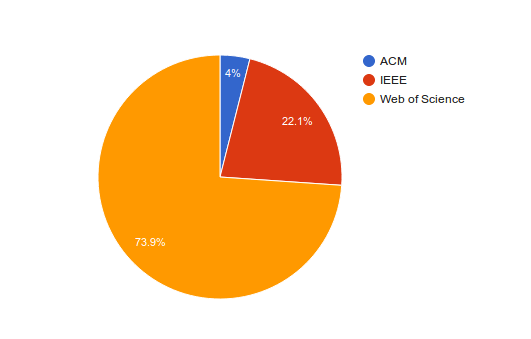
\includegraphics[width=1\textwidth]{fig/figura31.png}
\caption{Percentual dos resultados da execução do protocolo P1 por fonte de pesquisa.}
\label{fig:figure31}
\end{figure}

\subsection{Segunda Execução}

Na segunda execução, o objetivo foi buscar por teses e dissertações na Biblioteca Digital Brasileira de Teses e Dissertações (BDTD), que apresentassem pesquisas relacionadas a criação e aplicação  de processos de teste de software no contexto da indústria. Pesquisas, relacionadas à métodos ágeis e DevOps com aplicação prática mercado também foram considerados.

Para a segunda execução foram retornados 1126 referências, todas elas, teses e dissertações nos últimos cinco anos. 

\section{Seleção dos Estudos}
\label{sec:selecaodosestudos}

Na seleção dos estudos o objetivo é realizar uma categorização primária das pesquisas encontradas por meio da aplicação dos critérios de inclusão e exclusão definidos na subseção \ref{sec:criteriosdeselecao}. Essa categorização primária incidiu sob os resultados finais da primeira e segunda execução. A Tabela \ref{tab:3.1} apresenta o resultado quantitativo da identificação dos estudos (subseção \ref{sec:identificacaodosestudos}) realizado pelos protocolos P1 e P2.

\begin{table}[H]
\centering
\caption{Total de artigos, teses e dissertações identificados na pesquisa.}
\label{tab:3.1}
  \scalebox{0.75}{
\begin{tabular}{|c|c|c|c|c|}
\hline
\textbf{ACM} & \textbf{IEE} & \textbf{Web of Science} & \textbf{BDTD} & \textbf{Total} \\ \hline
20           & 112          & 374                     & 1126          & 1632           \\ \hline
\end{tabular}
}
\end{table}

Com a soma dos resultados encontrados na execução dos protocolos P1 e P2, total de 1632 (mil seiscentos e trinta e dois) artigos, foram analisados os resultados aplicando os critérios de inclusão e exclusão descrito na subseção \ref{sec:criteriosdeselecao}. Mais três categorias foram criadas para a realização da classificação dos resultados:

\begin{itemize}
\item [i] Artigos duplicados;
\item [ii] Artigos descartados (usando os critérios de exclusão);
\item [iv] Artigos aceitos (usando os critérios de inclusão).
\end{itemize}

As análises dos artigos foram realizadas sobe os resultados das máquinas de busca (Subseção \ref{sec:fontesdapesquisa}), neste caso, a cada execução foi selecionado um conjunto de trabalhos. A seleção foi realizada por uma leitura criteriosa do conteúdo dos resumos, títulos e palavras chaves dos artigos. Em alguns casos artigos exigiram uma leitura mais profunda afim de encontrar alguns dos aspectos definidos nos critérios de classificação.

\subsection{Exclusão de Estudos}
\label{sec:exclusaoestudos}

Artigos que se encaixavam nos critérios de exclusão (subseção \ref{sec:criteriosdeselecao}) ou duplicados foram excluídos desse estudo. Basicamente trabalhos relacionados à processos de teste sem estudo de caso e análise prática, artigos sobre DevOps e Métodos Ágeis com finalidades especificas e sem contexto da indústria ou conhecimento empírico também foram excluídos.

Em síntese os trabalhos examinados que não atendiam os critérios de seleção (subseção \ref{sec:criteriosdeselecao}) e que estavam nesse padrão, foram excluídos:

\begin{itemize}
\item Estudo científicos que abordam apenas processos de teste de software fora do contexto prático da indústria;
\item Estudo científicos que abordam processos de teste de software para uso especifico, como sistemas aviônicos, embarcados e críticos;
\item Estudo científicos que não abordam assuntos de teste de software;
\end{itemize}

\subsection{Estudos Aceitos}
\label{sec:estudosaceitos}
Os estudos aceitos neste trabalho adotaram o mesmo método de análise aplicado na subseção \ref{sec:criteriosdeselecao}. Foram utilizados os seguintes critérios de inclusão para realização das analises e classificações:

\begin{itemize}
\item Trabalhos com aplicação prática e/ou estudo de caso na indústria;
\item Trabalhos com ou sem estudo de caso voltadas para micro e pequenas empresas;
\item Revisões sistemáticas sobre processos de teste;
\item Processos  e  modelos  de  processo  já  conhecidos  pela  comunidade  acadêmica  e
indústria.
\end{itemize}

Após a realização das análises e agrupamento dos estudos em, teses e dissertações, artigos científicos, revisões sistemáticas e por fim processos de teste reconhecidos e mais citados nos trabalhos examinados, a tabela \ref{tab:3.2} foi criada listando os principais estudos que nortearam esse trabalho.

\begin{table*}[ht]
\centering
\caption{Quantitativo dos principais trabalhos aceitos para essa pesquisa.}
\label{tab:3.2}
  \scalebox{0.75}{
\begin{tabular}{|c|c|c|c|c|c|c|c|}
\hline \textbf{Teses e Dissertações } &\textbf{Revisões Sistemáticas} &\textbf{Artigos Científicos} &\textbf{Processos de Teste} \\ 
\hline 4 &2 &18 &6\\
\hline 
\end{tabular} 
}
\end{table*}

As discussões e trabalhos relacionados sobre os estudos selecionados serão melhor argumentados no item \ref{sec:discussoes}. Para facilitar o entendimento os estudos aceitos foram divididos de acordo com as categorias da tabela \ref{tab:3.2}.

\section{Discussões e Trabalhos Relacionados}
\label{sec:discussoes}

Os estudos aceitos e listados no item \ref{sec:estudosaceitos} serviram de embasamento principal para essa pesquisa e evidenciam o enfoque desse trabalho. As discussões realizadas aqui foram divididas pela categorização dos resultados da pesquisa como supramencionado no item anterior. Neste caso teses e dissertações, revisões sistemáticas, artigos científicos e processos de teste já reconhecidos pela comunidade acadêmica e da indústria.

\subsection{Teses e dissertações}
\label{sec:tesesdissertacoes}

O trabalho criação do arcabouço \textbf{KITest: Um arcabouço de conhecimento e melhoria de processo de teste} \cite{Nina2011} que funciona como um conjunto de ferramentas e técnicas “para agregar o conhecimento em teste e disponibilizá-lo para a comunidade com a intenção de facilitar a sua transferência, a definição e a melhoria de processos de teste, com mais qualidade”. 

Com aplicação do conhecimento abordado na pesquisa, a ferramenta KITTool foi criada com a intenção de auxiliar no diagnóstico de processos e orientar possíveis melhorias. Um processo genérico foi modelado baseado nas práticas do TMMi em formato de mapa mental, denominado KITMap.

O objetivo principal do arcabouço KITest (\textit{Knowledge and Improvement on Test}) é visto abaixo:

\begin{itemize}
\item Ter um módulo na criação do arcabouço KITest (\textit{Knowledge and Improvement on Test}) que funciona como um conjunto de ferramentas e técnicas "para agregar o conhecimento em teste e disponibilizá-lo para a comunidade com a intenção de facilitar a sua transferência, a definição e a melhoria de processos de teste, com mais qualidade".
\item Como aplicação do conhecimento abordado na pesquisa, a ferramenta KITTool foi criada com a intenção de auxiliar no diagnóstico de processos e orientar possíveis melhorias. Um processo genérico foi modelado baseado nas práticas do TMMi em formato de mapa mental, denominado KITMap.
\item Permitisse a centralização das informações sobre a atividade de teste, de uma maneira organizada, para facilitar a compreensão e a aquisição do conhecimento em teste;
\item Ter um módulo que viabilizasse a interação da comunidade com o módulo de conhecimento em teste, de forma que a comunidade fosse capaz de aplicar esse conhecimento na definição de um processo de teste com qualidade, seguindo as premissas de qualidade do TMMi, que concentra as melhores práticas existentes nessa área; e
\item Possuir um mecanismo que ajude a constante evolução desse conhecimento sobre teste, de forma que essa evolução fosse fundamentada na realimentação da comunidade, com base nos relatos de experiência sobre o uso das informações organizadas no módulo.
\end{itemize}

Conclui-se que a proposta do arcabouço KiTest é interessante no ponto de vista de disseminação de conhecimento em teste de software e uma ferramenta para nortear empresas/instituições de T.I. a alcançarem a maturidade desejada em seus Processos de Teste. Embora segundo a própria autora é necessário a aplicação e validação prática do arcabouço, nos estudos realizados dentro de uma experimentação controlada os resultados foram satisfatórios. Por fim, o arcabouço lida mais com aquisição de conhecimento em teste de software, avaliação do processo de teste de instituições da T.I., fazendo-se necessário da existência de pesquisas que auxiliem não somente no alinhamento da maturidade da empresa, como também pesquisas que corroborem a implantação das áreas de processo necessárias para se alcançar tais níveis de maturidade.

No trabalho \textbf{Um Arcabouço para Avaliação do Nível de Maturidade em Teste de Software para Micro e Pequenas Empresas} \cite{Araujo2013}, que apresenta um arcabouço validado na indústria para avaliação do nível de maturidade dos processos de teste das Micro e Pequenas Empresas com base nas boas práticas do TMMI. 

O autor utilizou da ajuda de questionários aplicados em diversas Micro e Pequenas Empresas do estado de Goiás para coletar dados inerentes à maturidade do processo de teste das empresas. Segundo o autor, o questionário evidenciou a carência das empresas do referido estado no sentido de boas práticas para o processo de teste. Todavia a pesquisa além de colaborar com uma métrica de maturidade dentro panorama do mercado de T.I pesquisado, ajudou a mostrar para as empresas a necessidade de melhorias.

A pesquisa \textbf{Melhoria do Processo de Teste para as Micro e Pequenas Empresas Brasileiras} \cite{SilvaDias2015} compara os processos de teste existentes na indústria brasileira e propõe melhorias do ponto de vista dos estudos realizados. 
A autora realiza comparações com iniciativas nacionais, como o Método FreeTest e MPT.Br para propor um modelo de maturidade considerando as limitações das micro e pequenas empresas de desenvolvimento de software, e uma abordagem para implementar os processos de teste definidos nesse modelo.

Apesar do levantamento \textit{in-loco} das informações de maturidade dos processos de teste de software das empresas e as propostas de melhoria para um processo, não houve validação prática do estudo. 

Outro estudo que corroborou substancialmente este trabalho foi o \textbf{Um Panorama Sobre o Uso de Práticas DevOps nas Indústrias de Software} \cite{BRAGA2015}, no qual o autor realiza um mapeamento sistemático do uso de práticas de DevOps na indústria. O autor elicita as práticas mais comuns utilizadas pelas empresas, realiza uma pesquisa utilizando questionários no mercado brasileiro de T.I. e como propostas de trabalhos futuros evidência a importância da criação de um processo de desenvolvimento que utilize práticas específicas de DevOps como um nicho de pesquisa.

\subsection{Processos de Teste MPT.Br e FreeTest}
\label{processosteste}

Processos são definidos por ações, observações e tomadas de decisões com a finalidade de obter um produto final como saída, sendo que, essas ações podem ocorrer em paralelo ou de forma sequencial. Processos de software agrega atividades, métodos bem como, as práticas utilizadas no desenvolvimento de um produto de software.

Para corroborar essa pesquisa os processos MPT.Br \cite{GuiaMPTbr} e o Método FreeTest \cite{Camilo-junior2012} foram analisados. Um processo bem definido e gerenciável permite que métricas e projetos de teste sejam facilmente alcançados com sucesso, a replicabilidade do processo é outro fator muito importante, pois é imprescindível que com um mesmo processo diferentes tipos de projetos possam ser executados. Com a análise dos dois processos e as inferências dos outros estudos avaliados pretende-se promover a melhoria do processo contido no Método FreeTest.

\subsection{MPT.Br}

O MPT.Br (Melhoria do Processo de Teste Brasileiro) \cite{GuiaMPTbr} foi concebido a fim de apoiar as organizações através de elementos essenciais da disciplina de teste. O MPT.Br como alguns outros processos de desenvolvimento de software nacionais foram inspirados no MPS.Br \cite{Softex} que por sua vez se inspirou no Modelo de Processo CMMI \cite{cmmi}. O MPT.Br aborda as melhores práticas envolvidas nas atividades inerentes à fase de teste de software de uma organização. Seu foco principal está em:

\begin{itemize}
    \item Ser um modelo de referência para a definição/implantação e melhoria do processo de teste das organizações;
    \item Melhoria contínua dos processos e aumento do nível de maturidade da empresa de acordo com suas necessidades;
    \item Boas práticas a serem empregadas ao longo da implementação do processo na organização. Sua divisão em Áreas de Processos, Atividades Especificas e práticas Genéricas contribuem para a implantação do processo.
\end{itemize}

O MPT.Br também foi concebido com base em modelos de referência em teste de software como, \textit{Testability Support Model (TSM)}, o \textit{Testing Maturity Model (TMM)}, a \textit{Test Process Improvement (TPI)}, a \textit{Test Organization Maturity (TOMtm)}, o \textit{Testing Assessement Program (TAP)}, o \textit{Testing Improvement Model (TIM)}, o \textit{Testing Maturity Model Integration (TMMI)}, o \textit{Maturity Model for Automated Software Testing}, o Modelo de Melhoria de Teste (MMT).

O MPT.Br é dividido em Áreas de Processo (AP), Práticas Especificas e Práticas Genéricas. Na tabela \ref{tab:3.3} pode ser visto tais itens dentro de seus respectivos níveis de maturidade.

\begin{table}[H]
\centering
\caption{Estrutura do MPT.Br \cite{GuiaMPTbr}.}
\label{tab:3.3}
  \scalebox{0.75}{
    \begin{tabular}{|l|l|l|l|}
    \hline
    \multicolumn{1}{|c|}{Nível de Maturidade} & \multicolumn{1}{c|}{Áreas de Processo} & \multicolumn{1}{c|}{Práticas Especificas} & \multicolumn{1}{c|}{Práticas Genéricas} \\ 
    \hline
    \multicolumn{1}{|c|}{Nível 1} & \multicolumn{1}{c|}{GPT} & \multicolumn{1}{c|}{GPT1 a GPT20} & \multicolumn{1}{c|}{PG1 a PG6} \\ 
    \cline{2-3}
    \multicolumn{1}{|c|}{} & \multicolumn{1}{c|}{PET} & \multicolumn{1}{c|}{PET1 a PET4} & \multicolumn{1}{c|}{} \\ 
    \hline
    \multicolumn{1}{|c|}{Nível 2} & \multicolumn{1}{c|}{GRT} & \multicolumn{1}{c|}{GRT1 a GRT5} & \multicolumn{1}{c|}{PG7 a PG9} \\ 
    \cline{2-3}
    \multicolumn{1}{|c|}{} & \multicolumn{1}{c|}{GRT} & \multicolumn{1}{c|}{GPT21 a GPT25} & \multicolumn{1}{c|}{} \\ 
    \cline{2-3}
    \multicolumn{1}{|c|}{} & \multicolumn{1}{c|}{PET} & \multicolumn{1}{c|}{PET5 a PET6} & \multicolumn{1}{c|}{} \\ 
    \hline
    \multicolumn{1}{|c|}{Nível 3} & \multicolumn{1}{c|}{FDT} & \multicolumn{1}{c|}{FDT1 a FDT4} & \multicolumn{1}{c|}{} \\ 
    \cline{2-3}
    \multicolumn{1}{|c|}{} & \multicolumn{1}{c|}{GDQ} & \multicolumn{1}{c|}{GDQ1 a GDQ3} & \multicolumn{1}{c|}{} \\ 
    \cline{2-3}
    \multicolumn{1}{|c|}{} & \multicolumn{1}{c|}{MAT} & \multicolumn{1}{c|}{MAT1 a MAT5} & \multicolumn{1}{c|}{} \\ 
    \cline{2-3}
    \multicolumn{1}{|c|}{} & \multicolumn{1}{c|}{OGT} & \multicolumn{1}{c|}{OGT1 a OGT10} & \multicolumn{1}{c|}{} \\ 
    \cline{2-3}
    \multicolumn{1}{|c|}{} & \multicolumn{1}{c|}{TDA} & \multicolumn{1}{c|}{TDA1 a TDA7} & \multicolumn{1}{c|}{} \\ 
    \cline{2-3}
    \multicolumn{1}{|c|}{} & \multicolumn{1}{c|}{TES} & \multicolumn{1}{c|}{TES1 a TES5} & \multicolumn{1}{c|}{} \\ 
    \cline{2-3}
    \multicolumn{1}{|c|}{} & \multicolumn{1}{c|}{TRE} & \multicolumn{1}{c|}{TRE1 a TRE4} & \multicolumn{1}{c|}{} \\ 
    \cline{2-3}
    \multicolumn{1}{|c|}{} & \multicolumn{1}{c|}{GPT} & \multicolumn{1}{c|}{GPT26 a GPT28} & \multicolumn{1}{c|}{} \\ 
    \cline{2-3}
    \multicolumn{1}{|c|}{} & \multicolumn{1}{c|}{PET} & \multicolumn{1}{c|}{GPT26 a GPT28} & \multicolumn{1}{c|}{} \\ 
    \hline
    \multicolumn{1}{|c|}{Nível 4} & \multicolumn{1}{c|}{AQP} & \multicolumn{1}{c|}{AQP1 a AQP5} & \multicolumn{1}{c|}{} \\ 
    \cline{2-3}
    \multicolumn{1}{|c|}{} & \multicolumn{1}{c|}{GDD} & \multicolumn{1}{c|}{GDD1 a GDD3} & \multicolumn{1}{c|}{} \\ 
    \cline{2-3}
    \multicolumn{1}{|c|}{} & \multicolumn{1}{c|}{TNF} & \multicolumn{1}{c|}{TNF1 a TNF3} & \multicolumn{1}{c|}{} \\ 
    \cline{2-3}
    \multicolumn{1}{|c|}{} & \multicolumn{1}{c|}{OGT} & \multicolumn{1}{c|}{OGT11 e OGT12} & \multicolumn{1}{c|}{} \\ 
    \hline
    \multicolumn{1}{|c|}{Nível 5} & \multicolumn{1}{c|}{AET} & \multicolumn{1}{c|}{AET1 a AET6} & \multicolumn{1}{c|}{} \\ 
    \cline{2-3}
    \multicolumn{1}{|c|}{} & \multicolumn{1}{c|}{CEP} & \multicolumn{1}{c|}{CEP1 a CEP5} & \multicolumn{1}{c|}{} \\ 
    \cline{2-3}
    \multicolumn{1}{|c|}{} & \multicolumn{1}{c|}{GDF} & \multicolumn{1}{c|}{GDF1 a GDF6} & \multicolumn{1}{c|}{} \\ 
    \hline
    \end{tabular}
}
\end{table}

A escolha do MPT.Br como base para essa pesquisa se dá pelo fato de que além de ser uma iniciativa nacional amplamente utilizada por Organizações e ser focado para o contexto de MPEs, o MPT.Br tem em sua estrutura dois componentes importantes: 

\begin{itemize}
    \item Modelo de Referência: Que apresenta a estrutura do processo, em áreas, práticas (especificas e genéricas) do nível de maturidade;
    \item Modelo de Avaliação: Aborda os critérios necessários para se avaliar um processo de teste de uma organização;
\end{itemize}

O MPT.Br possui um guia de Referência e de Avaliação que são de suma importância para guiar a empresa na implantação do processo de teste. Com a ajuda do Guia de Avaliação é possível que de tempos em tempos a Organização realiza avaliações de maturidade do seu processo e tome decisões para alcançar níveis mais altos ou ajustar alguma Área de Processo que não esteja como desejado. Apesar do MPT.Br ser proposto para organizações de todos os tamanhos e ser indicado para MPEs, o mesmo ainda possui muitas atividades que não estão totalmente alinhadas às necessidades de Organizações menores ou que desejam usar Métodos Ágeis. Logo nota-se uma oportunidade de melhoria, no refinamento da estrutura do Guia de Referência e também na necessidade de uma organização manter sempre seu processo em um nível de maturidade desejado.

\subsection{Método FreeTest}
\label{freetest}

O Método FreeTest \cite{Camilo-junior2012} surgiu como uma proposta completa para as Micro e Pequenas Empresas de T.I, pois desde a sua definição os autores do projeto se preocuparam com todas as necessidades que uma Organização teria, neste caso, um processo enxuto, ferramentas, técnicas e base de conhecimento para auxiliar as organizações à alcançarem o seu objetivo de maturidade. O projeto nasceu a partir do Estudo e Definição de Processo de Teste de Software para MPEs de TI, através do programa PAPPE Integração apoiado pela Fundação de Amparo à Pesquisa do Estado de Goiás (FAPEG)/Financiadora de Estudos e Projetos (FINEP) e, pelos pesquisadores do Instituto de Informática da Universidade Federal de Goiás (UFG) em conjunto com Organizações de T.I. do estado de Goiás \cite{Camilo-junior2012}.

O FreeTest foi inspirado em modelos de maturidade como TMMI e MPT.Br. De forma geral o Método consiste em um conjunto de processos, ferramentas e conhecimento em teste de software que estabelece uma solução de fácil aplicação para MPEs que desejam ter um processo de teste definido e/ou melhorar seus processos e ferramentas. A estrutura do Método FreeTest é mostrado na tabela \ref{tab:3.4}.


\begin{table}[H]
\centering
\caption{Estrutura do Método FreeTest \cite{Camilo-junior2012}.}
\label{tab:3.4}
  \scalebox{0.75}{
    \begin{tabular}{|l|l|l|}
    \hline
    \multicolumn{1}{|c|}{Nível de Maturidade} & \multicolumn{1}{c|}{Áreas de Processo} & \multicolumn{1}{c|}{Práticas Específicas} \\ 
    \hline
    \multicolumn{1}{|c|}{Nível A} & \multicolumn{1}{c|}{TPE} & \multicolumn{1}{c|}{TPE1 a TPE4} \\ 
    \hline
    \multicolumn{1}{|c|}{Nível B} & \multicolumn{1}{c|}{INC} & \multicolumn{1}{c|}{INC1 a INC3} \\ 
    \hline
    \multicolumn{1}{|c|}{Nível C} & \multicolumn{1}{c|}{TRG} & \multicolumn{1}{c|}{TRG1 a TRG4} \\ 
    \hline
    \multicolumn{1}{|c|}{Nível D} & \multicolumn{1}{c|}{TDA} & \multicolumn{1}{c|}{TDA1 a TDA3} \\ 
    \cline{2-3}
    \multicolumn{1}{|c|}{} & \multicolumn{1}{c|}{TRQ} & \multicolumn{1}{c|}{TRQ1 a TRQ2} \\ 
    \hline
    \multicolumn{1}{|c|}{Nível E} & \multicolumn{1}{c|}{TFU} & \multicolumn{1}{c|}{TFU1 a TFU3} \\ 
    \cline{2-3}
    \multicolumn{1}{|c|}{} & \multicolumn{1}{c|}{GPT} & \multicolumn{1}{c|}{GPT1} \\ 
    \hline
    \end{tabular}
    }
\end{table}

Como já mencionado o diferencial do Método FreeTest é sua abordagem enxuta e sua concepção. Para apoiar a rápida absorção das MPEs na implantação do Método FreeTest, três componentes foram construídos e distribuídos, que são:

\begin{itemize}
    \item Manual de Instalação, apoia na instalação do arcabouço;
    \item Manual de Utilização, que demonstra como realizar a integração entre ferramentas disponibilizadas.;
    \item Modelo de Processo, que consiste em toda a estrutura do FreeTest, com suas respectiva Áreas de Processos e práticas especificas.
\end{itemize}

O FreeTest assim como MPT.Br que são iniciativas nacionais de apoio a melhoria do processo de teste das Organizações de T.I. do Brasil abordam muitos fatores relevantes para o crescimento da maturidade em teste de software das organizações. No entanto, observando o cenário das MPEs que normalmente operam com um baixo custo de investimento e possuem limitações de profissionais capacitados, observa-se a necessidade de uma ferramenta que auxilie integralmente a implantação do processo e utilização de ferramentas. O FreeTest apesar de sua abordagem enxuta e oferta de ferramentas dentro do seu arcabouço, não apoia a implantação do processo de teste nas empresas, sendo muitas vezes necessário a contratação de profissionais qualificados para tal ou disponibilizar e mobilizar a organização para implantação do processo. Este estudo enxerga essa ausência, como uma oportunidade de pesquisa.

\section{Conclusões}
\label{sec:conclusoescap2}

Nas últimas décadas a comunidade científica tem tido um grande interesse em pesquisas sobre melhoria de processo de desenvolvimento de software. Neste entendimento, processos como ISO/IEC 12207 \cite{Mitasiunas2014}, RUP \cite{Veenendaal2012}, CMMI \cite{cmmi}, ProSoft \cite{Mitasiunas2014} o MPS.Br \cite{Softex}, e outros tem sido idealizados de modo a tentar reduzir os custos de produção das organizações e melhorar a eficiência das mesmas.

Diante desse grande cenário de oportunidade, modelos de processo de propósito específico foram criados para atender demandas emergentes e pontuais dentro dos modelos de processo de desenvolvimento de software. No contexto de teste de software, modelos como TMMi \cite{Veenendaal2012}, TPI \cite{Mitasiunas2014}, e a norma ISO/IEC 29119-2 \cite{Standard2013} vem sido estudados e estendidos no mundo todo para criação ou melhoria contínua de processo de uso específico na área de teste de software.

No estudo intitulado Modelos de Processo de Teste: Revisão Sistemática da Literatura (do inglês, \textit{Test Process Models: Systematic Literature Review} \cite{Carlo2010}) os autores realizaram uma a Revisão Sistemática em busca de responderem a seguinte pergunta: “Quais modelos de processos de teste de software foram definidos, adaptados ou estendidos na indústria de software de 1990 – 2014?”, dentre os resultados encontrados foram encontrados vinte e três modelos de processo, sendo que a maioria foi adaptada ou estendida de modelos como TMMi e TPI e norma ISO/IEC 29119. Dentro dos resultados relevantes desta pesquisa, as seguintes informações se destacaram:

\begin{itemize}
    \item Os modelos de Processo de Teste mais referenciados foram: TMMi e TPI;
    \item Treze modelos de processo de propósito geral foram encontrados;
    \item Nove modelos de processo de propósito especifico foram encontrados, sendo que, boa parte com foco em automação de teste de software, sistemas embarcados e Micro e Pequenas Empresas. Segundo o autor isso indica uma importante tendência de estudos \cite{Carlo2010}.
\end{itemize}

Por fim, através do embasamento nos estudos realizados e na carência de pesquisas que apoiem as atividades das MPEs no dia a dia, no sentido de obtenção de qualidade do produto de software desenvolvido. Também no que diz respeito em guiar as empresas na obtenção e manutenção de processos de teste ágeis e enxutos, a fim de, melhorar a qualidade do software produzido, principalmente no Brasil, este trabalho propõe, com base em todo a revisão da literatura feita neste capítulo melhorar o Método FreeTest, afim de agregar novos conceitos e tendências do mercado emergente contemporâneo, e junto a essas melhorias disponibilizar um guia de implantação para o processo, acompanhado de ferramentas de apoio criadas e disponibilizadas para a comunidade.
\chapter{Construção do Processo FreeTest 2.0}
\label{sec:construcaoframeworkprocesso}

Desde sua concepção o processo do Método FreeTest 1.0 propõe práticas, abordagens e técnicas alinhadas com a demanda crescente da indústria de tecnologia e estado da prática da literatura, com foco principal em Micro e Pequenas Empresas. 

Numa visão geral, o FreeTest 1.0 evoluiu de um modelo “Cascata-Ágil“ (\textit{Fast Waterfall}) para um modelo “Ágil“, contudo com uma Integração Contínua (\textit{Continuous Integration}) mais modesta \cite{sauceLabes2017}. Este capítulo propõe melhorar o processo, nomeando-o como, “\textbf{FreeTest 2.0}“ e trazendo abordagens mais aderente às técnicas ágeis, integração contínua e inserindo práticas que contemplem um modelo de processo do tipo “Entrega Contínua“ (\textit{Continuous Delivery}). As melhorias propostas neste capítulo são com base nas revisões da literatura (capítulo \ref{sec:referencialteorico}) e conhecimento empírico dos pesquisadores. Este capítulo está organizado da seguinte forma:

\begin{itemize}
    \item Na subseção \ref{sec:identificacaomelhoriasfreetest}, os estudos com embasamento teórico são mostrados com a intenção de evidenciar as possíveis melhorias para o novo processo;
    \item Na subseção \ref{sec:melhoriaspropostas}, é elicitado as melhorias propostas para o processo FreeTest 2.0;
    \item Na subseção \ref{sec:areasdeprocessoepraticas}, são listados as Áreas de Processo (AP's) e Práticas Especificas (PE's) de forma detalhada;
    \item Na subseção \ref{sec:consideracoesfinaiscap4}, uma explanação e sintetização desse capítulo é realizada.
\end{itemize}

%Construção do processo FreeTest 2.0
\section{Identificação de melhorias no Método FreeTest 1.0}
\label{sec:identificacaomelhoriasfreetest}

Para que essa pesquisa fosse conduzida e eventuais melhorias no processo do Método FreeTest 1.0 fossem realizadas, foi necessário um estudo do estado da prática (capítulo \ref{sec:referencialteorico}) de processos de teste já consolidados, artigos científicos, teses e dissertações que abordassem processos de teste com aplicação prática, estudo de caso e validações em ambientes controlados. Diante disso, após essa análise dos estudos e utilizando o embasamento teórico do capítulo \ref{sec:referencialteorico}, foram realizadas análises comparativas entre o Método FreeTest 1.0 e MPT.Br \cite{GuiaMPTbr}, e por fim, adição de práticas especificas dentro do processo, que são inerentes ao contexto de DevOps \cite{Debois2008} e Métodos Ágeis \cite{Beck2001}. 

Com a finalidade de comparar os processos e sugerir adições ou remoções no mesmo, foi realizado um mapeamento de equivalência entre o Método FreeTest 1.0 e MPT.Br exibido na tabela \ref{tab:4.1}, esse mapeamento mostra as práticas especificas existentes no FreeTest 1.0 que o MPT.Br possui de forma equivalente. Uma tabela (\ref{tab:4.2}) que contém as atividades do FreeTest 1.0 que não possuem equivalência com o MPT.Br também foi criada para contribuir na análise entre os dois processos.

\begin{table}[!ht]
\centering
\caption{Mapeamento de equivalências entre o FreeTest 1.0 e MPT.Br}
\label{tab:4.1}
\begin{tabular}{|c|l|l|c|}
\hline
\multicolumn{2}{|c|}{\textbf{FreeTest 1.0}}             & \multicolumn{2}{c|}{\textbf{MPT.Br}}           \\ \hline
\textbf{AP}          & \multicolumn{1}{c|}{\textbf{PE}} & \multicolumn{1}{c|}{\textbf{AP}} & \textbf{PE} \\ \hline
GPT                  & GPT1                             & \multirow{2}{*}{GPT}             & GPT14       \\ \cline{1-2} \cline{4-4} 
\multirow{3}{*}{TFU} & TFU1                             &                                  & GPT11       \\ \cline{2-4} 
                     & TFU2                             & PET                              & PET2 a PET4 \\ \cline{2-4} 
                     & TFU3                             & FDT                              & FDT4        \\ \hline
\multirow{2}{*}{TRQ} & TRQ1                             & \multirow{2}{*}{TES}             & TES1 a TES3 \\ \cline{2-2} \cline{4-4} 
                     & TRQ2                             &                                  & TES4        \\ \hline
\multirow{3}{*}{TDA} & TDA1                             & \multirow{3}{*}{TDA}             & TDA5        \\ \cline{2-2} \cline{4-4} 
                     & TDA2                             &                                  & TDA6        \\ \cline{2-2} \cline{4-4} 
                     & TDA3                             &                                  & TDA7        \\ \hline
\end{tabular}
\end{table}


\begin{table}[!ht]
\centering
\caption{Práticas especificas do Método FreeTest 1.0 que não possuem equivalência com o MPT.Br.}
\label{tab:4.2}
\begin{tabular}{|c|l|}
\hline
\multicolumn{2}{|c|}{\textbf{FreeTest 1.0}}                                     \\ \hline
Área de Processo                     & \multicolumn{1}{c|}{Práticas Especificas} \\ \hline
\multirow{4}{*}{Teste de regressão}  & Preparar massa de teste (TRG1)            \\ \cline{2-2} 
                                     & Manter \textit{script} de regressão (TRG2)         \\ \cline{2-2} 
                                     & Executar teste de regressão (TRG3)        \\ \cline{2-2} 
                                     & Encerrar teste de regressão (TRG4)        \\ \hline
\multirow{3}{*}{Integração contínua} & Elaborar código (INC1)                    \\ \cline{2-2} 
                                     & Elaborar \textit{script} BDD (INC2)                \\ \cline{2-2} 
                                     & Montar \textit{build} (INC3)                       \\ \hline
\multirow{4}{*}{Teste de desempenho} & Preparar massa de teste (TPE1)            \\ \cline{2-2} 
                                     & Manter \textit{script} de desempenho (TPE2)        \\ \cline{2-2} 
                                     & Executar teste de desempenho (TPE3)       \\ \cline{2-2} 
                                     & Encerrar teste de desempenho (TPE4)       \\ \hline
\end{tabular}
\end{table}

Como observados na tabela \ref{tab:4.2} somente as Práticas Especificas (PE) e Áreas de Processo (AP) do Método FreeTest 1.0 que não possuem quaisquer equivalências com as práticas especificas do MPT.Br foram ressaltadas. Na tabela \ref{tab:4.1} as práticas especificas do FreeTest 1.0 que possuem equivalência com o MPT.Br foram listadas, a intenção é que somente as práticas especificas do MPT.Br que não foram listadas sejam possíveis contribuições de melhoria ao FreeTest 2.0.

Diante da revisão da literatura e referencial teórico no capítulo \ref{sec:referencialteorico}, algumas propostas de mudança no processo foram elencadas de acordo com as boas práticas da Metodologia Ágil \cite{Beck2001,Debois2008} e Devops \cite{Howlett,Fitzgerald2014,Erich2014}, como as listadas a seguir:

\begin{itemize}
    \item Testes Unitários (\textit{Unit Testing});
    \item Testes de Fumaça (\textit{Smoke Testing / Build Verification Test});
    \item Testes de Integração (\textit{Integration Testing});
    \item Testes de Sistema (\textit{System Testing});
    \item Testes Exploratórios (\textit{Exploratory Testing});
    \item Testes de Aceitação (\textit{Storytesting / Acceptance Criteria / Acceptance Testing});
    \item Testes contínuos (\textit{Continuos Testing});
    \item Infraestrutura como código (\textit{Infrastructure as Code})\cite{BRAGA2015};
\end{itemize}

Na seção \ref{sec:melhoriaspropostas} será apresentado as melhorias propostas para o FreeTest 2.0. O mapeamento incluirá a adição, permanência e remoção das práticas especificas para o processo proposto.

\section{Melhorias propostas para o processo}
\label{sec:melhoriaspropostas}

Para propor as melhorias para o processo do Método FreeTest 2.0 foi necessário a elaboração de um mapeamento das equivalências identificadas entre as práticas especificas do Método FreeTest 1.0 e MPT.Br, e revisão da literatura na perspectiva da Metodologia Ágil e das boas práticas empregadas no Devops (subseção \ref{sec:identificacaomelhoriasfreetest}).
A abordagem utilizada para a tomada de decisão de quais práticas especificas seriam mantidas, incluídas ou removidas para o processo do FreeTest 1.0 foi o contexto no qual ele se emprega, ou seja, as Micro e Pequenas Empresas, sendo assim, alguns critérios de seleção foram adotados com base no conhecimento empírico do autor e da literatura \cite{JamesWhittakerJasonCarollo2012, Especialistas2015, Whittaker2009, ABESSofftware2014, FelipeDreher2016, Laporte2010, Ramachandram2008, SilvaDias2015}, para ajudar nas decisões no contexto das MPEs:

\begin{itemize}
    \item Soluções de baixo custo de aquisição e implantação;
    \item Equipes enxutas. Por exemplo, muitas vezes o gestor gere tanto a equipe de teste quanto de desenvolvimento;
    \item Não existem políticas de teste ou organizacionais bem definidas;
    \item Não existe tanta burocracia e muitas pessoas tem poder de decisão;
    \item Projetos de software menores ou softwares de prateleira;
    \item Poucos analistas seniores, geralmente o sócio fundador é o que entende mais do software/código fonte;
    \item Comunicação mais ágil e pontual, sem muita formalização ou documentação;
    \item Baixa documentação de software e de requisitos;
    \item Baixo orçamento para aquisição de ferramentas de trabalho e licenças de software mais caras;
    \item Processos de desenvolvimento e teste não definidos, muitas vezes processos diferentes para clientes diferentes.
\end{itemize}

Nas tabelas \ref{tab:4.3} e \ref{tab:4.4} é possível observar as sugestões de melhoria a partir do MPT.Br e FreeTest 1.0 para o processo FreeTest 2.0. É importante salientar que as práticas especificas avaliadas, tanto do processo MPT.Br e Método FreeTest 1.0 sofreram uma avaliação do tipo, “Mantido“, “Excluído“ ou “Adicionado“ como observado nas tabelas. 

\begin{table}[!ht]
\centering
\caption{Sugestões de melhoria para o FreeTest 2.0 a partir do MPT.Br}
\label{tab:4.3}
\scalebox{0.75}{
    \begin{tabular}{|l|l|l|}
    \hline
    \multicolumn{1}{|c|}{Área de Processo} & \multicolumn{1}{c|}{Prática Especifica} & \multicolumn{1}{c|}{Ação} \\ 
    \hline
    \multicolumn{1}{|c|}{GPT} & GPT1 – Realizar análise de risco do produto & \multicolumn{1}{c|}{Adicionado} \\ 
    \cline{2-3}
    \multicolumn{1}{|c|}{} & GPT3 – Definir estratégia de teste & \multicolumn{1}{c|}{Adicionado} \\ 
    \cline{2-3}
    \multicolumn{1}{|c|}{} & GPT4 – Definir o escopo do trabalho para o projeto de teste & \multicolumn{1}{c|}{Adicionado} \\ 
    \cline{2-3}
    \multicolumn{1}{|c|}{} & GPT5 – Estabelecer estimativas de tamanho & \multicolumn{1}{c|}{Adicionado} \\ 
    \cline{2-3}
    \multicolumn{1}{|c|}{} & GPT7 – Estimar o esforço e o custo & \multicolumn{1}{c|}{Adicionado} \\ 
    \cline{2-3}
    \multicolumn{1}{|c|}{} & GPT9 – Identificar riscos do projeto & \multicolumn{1}{c|}{Adicionado} \\ 
    \cline{2-3}
    \multicolumn{1}{|c|}{} & GPT10 – Planejar os recursos humanos & \multicolumn{1}{c|}{Adicionado} \\ 
    \cline{2-3}
    \multicolumn{1}{|c|}{} & GPT11 – Planejar o ambiente de teste para o projeto & \multicolumn{1}{c|}{Mantido} \\ 
    \cline{2-3}
    \multicolumn{1}{|c|}{} & GPT12 – Planejar os artefatos e dados do projeto & \multicolumn{1}{c|}{Adicionado} \\ 
    \cline{2-3}
    \multicolumn{1}{|c|}{} & GPT14 – Estabelecer o Plano de Teste & \multicolumn{1}{c|}{Mantido} \\ 
    \cline{2-3}
    \multicolumn{1}{|c|}{} & GPT16 – Monitorar o projeto & \multicolumn{1}{c|}{Adicionado} \\ 
    \cline{2-3}
    \multicolumn{1}{|c|}{} & GPT24 – Monitorar defeitos & \multicolumn{1}{c|}{Adicionado} \\ 
    \hline
    \multicolumn{1}{|c|}{PET} & PET1 – Identificar casos de teste & \multicolumn{1}{c|}{Adicionado} \\ 
    \cline{2-3}
    \multicolumn{1}{|c|}{} & PET2 – Executar casos de teste & \multicolumn{1}{c|}{Mantido} \\ 
    \cline{2-3}
    \multicolumn{1}{|c|}{} & PET3 – Reportar incidentes & \multicolumn{1}{c|}{Mantido} \\ 
    \cline{2-3}
    \multicolumn{1}{|c|}{} & PET4 – Acompanhar incidentes & \multicolumn{1}{c|}{Mantido} \\ 
    \hline
    \multicolumn{1}{|c|}{FDT} & FDT4 – Consolidar dados de teste & \multicolumn{1}{c|}{Mantido} \\ 
    \hline
    \multicolumn{1}{|c|}{MAT} & MAT1 – Definir objetivos de medição de teste & \multicolumn{1}{c|}{Adicionado} \\ 
    \cline{2-3}
    \multicolumn{1}{|c|}{} & MAT4 – Coletar, analisar e comunicar dados de medição & \multicolumn{1}{c|}{Adicionado} \\ 
    \cline{2-3}
    \multicolumn{1}{|c|}{} & MAT5 – Armazenar dados de medição & \multicolumn{1}{c|}{Adicionado} \\ 
    \hline
    \multicolumn{1}{|c|}{OGT} & OGT1 – Definir a estrutura organizacional do teste & \multicolumn{1}{c|}{Adicionado} \\ 
    \cline{2-3}
    \multicolumn{1}{|c|}{} & OGT2 – Estabelecer um Grupo de processo de teste de software & \multicolumn{1}{c|}{Adicionado} \\ 
    \cline{2-3}
    \multicolumn{1}{|c|}{} & OGT6 – Coletar informações e implementar ações de melhoria & \multicolumn{1}{c|}{Adicionado} \\ 
    \cline{2-3}
    \multicolumn{1}{|c|}{} & OGT11 – Identificar oportunidades de reuso & \multicolumn{1}{c|}{Adicionado} \\ 
    \cline{2-3}
    \multicolumn{1}{|c|}{} & OGT12 – Reusar ativos de teste & \multicolumn{1}{c|}{Adicionado} \\ 
    \hline
    \multicolumn{1}{|c|}{TDA} & TDA5 – Preparar ambiente para aceitação & \multicolumn{1}{c|}{Mantido} \\ 
    \cline{2-3}
    \multicolumn{1}{|c|}{} & TDA6 – Conduzir testes de aceitação & \multicolumn{1}{c|}{Mantido} \\ 
    \cline{2-3}
    \multicolumn{1}{|c|}{} & TDA7 – Avaliar condições de aceitação & \multicolumn{1}{c|}{Mantido} \\ 
    \hline
    \multicolumn{1}{|c|}{TES} & TES1 – Identificar produtos de trabalho e tipos de revisão & \multicolumn{1}{c|}{Excluído} \\ 
    \cline{2-3}
    \multicolumn{1}{|c|}{} & TES2 – Definir critérios de revisões & \multicolumn{1}{c|}{Excluído} \\ 
    \cline{2-3}
    \multicolumn{1}{|c|}{} & TES3 – Conduzir revisões & \multicolumn{1}{c|}{Excluído} \\ 
    \cline{2-3}
    \multicolumn{1}{|c|}{} & TES4 – Analisar dados de revisões & \multicolumn{1}{c|}{Excluído} \\ 
    \hline
    \multicolumn{1}{|c|}{AET} & AET3 – Definir um \textit{framework} para automação de teste & \multicolumn{1}{c|}{Adicionado} \\ 
    \cline{2-3}
    \multicolumn{1}{|c|}{} & AET4 – Gerenciar incidentes de teste automatizado & \multicolumn{1}{c|}{Adicionado} \\ 
    \hline
    \end{tabular}
}
\end{table}


\begin{table}[H]
\centering
\caption{Melhorias promovidas para o FreeTest 2.0 a partir das práticas do FreeTest 1.0}
\label{tab:4.4}
\begin{tabular}{|c|l|c|}
\hline
\textbf{Área de Processo}                                 & \multicolumn{1}{c|}{\textbf{Prática Especifica}} & \textbf{Ação}                 \\ \hline
\multirow{4}{*}{Teste de regressão}                       & Preparar massa de teste (TRG1)                   & Mantida                       \\ \cline{2-3} 
                                                          & Manter script de regressão (TRG2)                & Mantida                       \\ \cline{2-3} 
                                                          & Executar teste de regressão (TRG3)               & Mantida                       \\ \cline{2-3} 
                                                          & Encerrar teste de regressão (TRG4)               & Mantida                       \\ \hline
\multirow{3}{*}{Integração contínua}                      & Elaborar código (INC1)                           & Mantida                       \\ \cline{2-3} 
                                                          & Elaborar script BDD (INC2)                       & Excluído                      \\ \cline{2-3} 
                                                          & Montar build (INC3)                              & Mantida                       \\ \hline
\multirow{4}{*}{Teste de desempenho}                      & Preparar massa de teste (TPE1)                   & Mantida                       \\ \cline{2-3} 
                                                          & Manter script de desempenho (TPE2)               & Mantida                       \\ \cline{2-3} 
                                                          & Executar teste de desempenho (TPE3)              & Mantida                       \\ \cline{2-3} 
                                                          & Encerrar teste de desempenho (TPE4)              & Mantida                       \\ \hline
\multicolumn{1}{|l|}{\multirow{2}{*}{Teste de Requisito}} & Realizar verificação (TRQ1)                      & \multicolumn{1}{l|}{Excluído} \\ \cline{2-3} 
\multicolumn{1}{|l|}{}                                    & Encerrar verificação (TRQ2)                      & \multicolumn{1}{l|}{Excluído} \\ \hline
\end{tabular}
\end{table}

Com base nos critérios de análise elencados no inicio desta seção, as tabelas \ref{tab:4.3} e \ref{tab:4.4} mostram os resultados das contribuições para a melhoria do FreeTest 2.0 na perspectiva do MPT.Br e FreeTest 1.0. Conforme já mencionado, além dos critérios de análise baseado no contexto e visita a algumas MPEs, foram utilizados critérios que corroboram com o uso de Metodologias Ágeis e DevOps (seção \ref{sec:identificacaomelhoriasfreetest}). Devido ao perfil atual das MPEs foi necessário a junção de algumas práticas especificas citadas no MPT.Br, de modo que a sua execução por parte das MPEs fossem realizadas de forma mais fácil e menos onerosa. Outra decisão tomada foi a alteração do nível de maturidade de determinadas práticas especificas utilizadas, tanto do MPT.Br quanto do FreeTest 1.0, a intenção foi mantê-los em um nível de maturidade que estivesse mais atrelado à situação atual das MPEs nacionais \cite{Especialistas2015, SilvaDias2015} e dos estudos realizados.

Como é possível verificar na tabela \ref{tab:4.5}, que mostra o resultado das análises e contribuições do MPT.Br, FreeTest 1.0, Métodos Ágeis e DevOps para o FreeTest 2.0, a coluna “Nível de Maturidade FreeTest 2.0“ mostra o nível de maturidade no qual a prática especifica corresponde no processo FreeTest 2.0, “AP“ é o nome da área de processo, “PE“ é o nome da prática especifica, “Nível de Maturidade da Fonte“ é o nível de maturidade (quando havia) no qual a prática especifica tanto do MPT.Br quanto do FreeTest 1.0 pertencia, e por fim as práticas especificas (quando havia) relacionadas à criação da nova prática. É importante salientar que nem todas práticas especificas abordadas no MPT.Br e no FreeTest 1.0 foram mantidas para essa nova abordagem (vide tabelas \ref{tab:4.3} e \ref{tab:4.4}).

\begin{table}[H]
\centering
\caption{Proposta para o FreeTest 2.0: Readaptação com a junção de práticas, alteração de nível de maturidade e inserção de novas práticas especificas.}
\label{tab:4.5}
\scalebox{0.70}{
\begin{tabular}{|c|c|c|c|c|c|}
\hline
\textbf{\begin{tabular}[c]{@{}c@{}}Nível de\\ Maturidade\\ FreeTest 2.0\end{tabular}} & \textbf{AP}                               & \textbf{PE}               & \textbf{Origem}                  & \textbf{\begin{tabular}[c]{@{}c@{}}Nível de Maturidade\\ da Fonte\end{tabular}} & \textbf{\begin{tabular}[c]{@{}c@{}}Práticas Especificas\\ Relacionadas\end{tabular}} \\ \hline
\multirow{10}{*}{1}                                                                   & \multirow{5}{*}{GPT}                      & GPT1                      & MPT.Br                           & 1                                                                               & GPT1, GPT3, GPT9                                                                     \\ \cline{3-6} 
                                                                                      &                                           & GPT2                      & MPT.Br                           & 1                                                                               & GPT4                                                                                 \\ \cline{3-6} 
                                                                                      &                                           & GPT3                      & MPT.Br                           & 1                                                                               & GPT5,GPT11, GPT12                                                                    \\ \cline{3-6} 
                                                                                      &                                           & GPT4                      & MPT.Br                           & 1                                                                               & GPT3, GPT7                                                                           \\ \cline{3-6} 
                                                                                      &                                           & GPT5                      & MPT.Br                           & 1                                                                               & GPT16                                                                                \\ \cline{2-6} 
                                                                                      & \multirow{5}{*}{ET}                       & ET1                       & MPT.Br                           & 1                                                                               & PET1                                                                                 \\ \cline{3-6} 
                                                                                      &                                           & ET2                       & DevOps                           & -                                                                               & -                                                                                    \\ \cline{3-6} 
                                                                                      &                                           & ET3                       & MPT.Br                           & 1                                                                               & PET2                                                                                 \\ \cline{3-6} 
                                                                                      &                                           & ET4                       & MPT.Br                           & 1                                                                               & PET3, PET4                                                                           \\ \cline{3-6} 
                                                                                      &                                           & ET5                       & FreeTest 1.0                     & 1                                                                               & FDT4                                                                                 \\ \hline
\multirow{10}{*}{2}                                                                   & \multicolumn{1}{l|}{\multirow{3}{*}{TDA}} & \multicolumn{1}{l|}{TDA1} & DevOps                           & -                                                                               & -                                                                                    \\ \cline{3-6} 
                                                                                      & \multicolumn{1}{l|}{}                     & \multicolumn{1}{l|}{TDA2} & FreeTest 1.0                     & 2                                                                               & TDA2                                                                                 \\ \cline{3-6} 
                                                                                      & \multicolumn{1}{l|}{}                     & \multicolumn{1}{l|}{TDA3} & FreeTest 1.0                     & 2                                                                               & TDA3                                                                                 \\ \cline{2-6} 
                                                                                      & \multirow{3}{*}{AES}                      & AES1                      & MPT.Br                           & 3                                                                               & TES1, TES2                                                                           \\ \cline{3-6} 
                                                                                      &                                           & AES2                      & MPT.Br                           & 3                                                                               & TES3                                                                                 \\ \cline{3-6} 
                                                                                      &                                           & AES3                      & Método Ágil                      & -                                                                               & -                                                                                    \\ \cline{2-6} 
                                                                                      & \multicolumn{1}{l|}{\multirow{4}{*}{TRG}} & TRG1                      & FreeTest 1.0                     & 3                                                                               & TRG1                                                                                 \\ \cline{3-6} 
                                                                                      & \multicolumn{1}{l|}{}                     & TRG2                      & FreeTest 1.0                     & 3                                                                               & TRG2                                                                                 \\ \cline{3-6} 
                                                                                      & \multicolumn{1}{l|}{}                     & TRG3                      & FreeTest 1.0                     & 3                                                                               & TRG3                                                                                 \\ \cline{3-6} 
                                                                                      & \multicolumn{1}{l|}{}                     & TRG4                      & FreeTest 1.0                     & 3                                                                               & TRG4                                                                                 \\ \hline
\multirow{9}{*}{3}                                                                    & \multirow{3}{*}{AET}                      & AET1                      & MPT.Br                           & 5                                                                               & AET2                                                                                 \\ \cline{3-6} 
                                                                                      &                                           & AET2                      & MPT.Br                           & 5                                                                               & AET3                                                                                 \\ \cline{3-6} 
                                                                                      &                                           & AET3                      & MPT.Br                           & 5                                                                               & AET4                                                                                 \\ \cline{2-6} 
                                                                                      & \multirow{3}{*}{GCT}                      & GCT1                      & MPT.Br                           & 4                                                                               & OGT11, OGT12                                                                         \\ \cline{3-6} 
                                                                                      &                                           & \multicolumn{1}{l|}{GCT2} & MétodoÁgil                       & -                                                                               & -                                                                                    \\ \cline{3-6} 
                                                                                      &                                           & \multicolumn{1}{l|}{GCT3} & DevOps                           & -                                                                               & -                                                                                    \\ \cline{2-6} 
                                                                                      & \multirow{3}{*}{MED}                      & MED1                      & MPT.Br                           & 3                                                                               & MAT1                                                                                 \\ \cline{3-6} 
                                                                                      &                                           & MED2                      & MPT.Br                           & 3                                                                               & MAT4                                                                                 \\ \cline{3-6} 
                                                                                      &                                           & MED3                      & MPT.Br                           & 3                                                                               & MAT5                                                                                 \\ \hline
\multirow{8}{*}{4}                                                                    & \multirow{4}{*}{INC}                      & INC1                      & FreeTest 1.0                     & 4                                                                               & INC3                                                                                 \\ \cline{3-6} 
                                                                                      &                                           & INC2                      & Método Ágil                      & -                                                                               & -                                                                                    \\ \cline{3-6} 
                                                                                      &                                           & INC3                      & Método Ágil                      & -                                                                               & -                                                                                    \\ \cline{3-6} 
                                                                                      &                                           & INC4                      & Método Ágil                      & -                                                                               & -                                                                                    \\ \cline{2-6} 
                                                                                      & \multirow{4}{*}{TEP}                      & TPE1                      & FreeTest                         & 5                                                                               & TPE1                                                                                 \\ \cline{3-6} 
                                                                                      &                                           & TPE2                      & FreeTest                         & 5                                                                               & TPE2                                                                                 \\ \cline{3-6} 
                                                                                      &                                           & TPE3                      & FreeTest                         & 5                                                                               & TPE3                                                                                 \\ \cline{3-6} 
                                                                                      &                                           & TPE4                      & FreeTest                         & 5                                                                               & TPE4                                                                                 \\ \hline
\multirow{7}{*}{5}                                                                    & \multicolumn{1}{l|}{\multirow{4}{*}{TCA}} & \multicolumn{1}{l|}{TCA1} & \multicolumn{1}{l|}{Método Ágil} & -                                                                               & -                                                                                    \\ \cline{3-6} 
                                                                                      & \multicolumn{1}{l|}{}                     & \multicolumn{1}{l|}{TCA2} & \multicolumn{1}{l|}{Método Ágil} & -                                                                               & -                                                                                    \\ \cline{3-6} 
                                                                                      & \multicolumn{1}{l|}{}                     & \multicolumn{1}{l|}{TCA3} & \multicolumn{1}{l|}{Método Ágil} & -                                                                               & -                                                                                    \\ \cline{3-6} 
                                                                                      & \multicolumn{1}{l|}{}                     & \multicolumn{1}{l|}{TCA4} & \multicolumn{1}{l|}{Método Ágil} & -                                                                               & -                                                                                    \\ \cline{2-6} 
                                                                                      & \multirow{3}{*}{OT1}                      & OT1                       & MPT.Br                           & 4                                                                               & OGT1                                                                                 \\ \cline{3-6} 
                                                                                      &                                           & OT2                       & MPT.Br                           & 4                                                                               & OGT2                                                                                 \\ \cline{3-6} 
                                                                                      &                                           & OT3                       & MPT.Br                           & 4                                                                               & OGT6                                                                                 \\ \hline
\end{tabular}
}
\end{table}


Analisando os resultados sugeridos para o FreeTest 2.0, exibidos na tabela \ref{tab:4.5} a AP de Gerenciamento de Projetos de Teste (GPT), por exemplo, foi a que mais sofreu alterações. Como as MPEs possuem equipes reduzidas de teste, normalmente a gestão dos projetos de teste ocorre juntamente com a gestão do projeto de desenvolvimento. Desta forma, foi necessário adicionar algumas práticas especificas oriundas do MPT.Br, principalmente como apoio ao planejamento do projeto, neste caso as práticas especificas GPT1, GPT2, GPT3, GPT4 e GPT5 que contribuem para a análise de risco, definição de estratégias de teste, escopo de testes e geram insumos para a criação de cronogramas, alocação de recursos humanos e monitoramento do projeto. Tais práticas, podem ser realizadas com o apoio do gerente de projetos e/ou líder técnico da equipe de teste, no entanto, se realizado por toda a equipe no inicio e durante o projeto, a execução desta prática torna a equipe mais engajada e cria responsabilidades mútuas à todos os envolvidos. 

A AP de Execução de Testes (ET) não sofreu alterações de nível de maturidade, no entanto, foram acrescentadas algumas práticas especificas como, ET1 e ET4 oriundas do MTB.Br, que apoiam na identificação de casos de teste e reportar e acompanhar incidentes, respectivamente. Sendo a última, uma junção de duas práticas especificas, PET3 e PET4 do MPT.Br. Outra contribuição para a AP de Execução de Testes foi a introdução de uma nova abordagem para a criação/atualização de ambientes de teste, agora com o uso de boas práticas em DevOps, com o foco em criação da infraestrutura de testes virtualizadas e “como serviço“, com a proposta de economizar em recursos computacionais e manter os ambientes de testes versionados, já que poderão ser mantidos em \textit{containers} \cite{BRAGA2015}.

Uma mudança importante foi definir as atividades de Análise Estática (AES), normalmente realizadas no nível três de maturidade do MPT.Br para o nível dois de maturidade do FreeTest 2.0. Essa iniciativa surgiu, pois as atividades de revisão costumam ser de baixo custo e facilmente automatizadas (exemplo, análise estática de código), neste sentido são práticas especificas eficazes e que evidenciam erros numa fase primária de codificação, ideal para o contexto das MPEs e como sugere a Metodologia Ágil \cite{Beck2001}. A área de processo de Teste de Aceite (TDA) foi mantida conforme estava no FreeTest 1.0, exceto pela alteração da prática especifica TDA1, de criação/atualização de ambiente de aceitação, que passou por melhorias com a inserção de práticas sugeridas pelo DevOps \cite{Howlett}. E por fim, o nível dois de maturidade do FreeTest 2.0 agora aborda também a AP de Teste de Regressão (TRG), que se manteve da mesma forma que na versão anterior, contudo antes era proposta no nível três de maturidade e agora é indicada no nível dois.

As práticas especificas AET1, AET2 e AET3 que abordam a AP de Automação da Execução dos Testes (AET) também sofreram grande mudança, pois no MPT.Br elas são aplicadas no nível cinco de maturidade, contudo na proposta para o FreeTest 2.0 tais práticas são sugeridas no nível três de maturidade. Essa mudança ocorreu, pois a automação é uma prática muito recomendada e difundida, apesar de ser vista como uma prática muitas vezes onerosa e de retorno de investimento a médio/longo prazo, no entanto, com os avanços de ferramentas e técnicas de automação é possível a implantação de uma automação com baixo custo e muito eficiente \cite{humble2010}. Com isso, as MPEs podem reduzir os recursos humanos e seus custos, fundamental para esse contexto. 

Outras duas APs foram adicionadas ao nível três de maturidade do FreeTest 2.0, as áreas de processo de Gerência de Configuração de Teste (GCT) e Medição (MED). Embora o gerenciamento de configuração ocorra de forma transversal a todo o projeto de desenvolvimento, é importante destacar o versionamento dos artefatos, \textit{scripts} (prática especifica GCT1), infraestrutura virtualizada dos ambientes de teste (prática especifica GCT3) e a criação de linhas de base de artefatos (prática especifica GCT2). O versionamento correto, possibilita o reúso e base histórica, desta maneira contribuindo com a evolução do processo e reduzindo custos com a reutilização de \textit{scripts}. A AP de Medição mesmo no contexto das MPEs que normalmente não possuem grande quantidade de documentação é importante, pois é necessário que haja uma estratégia para extrair dados que sejam utilizados como objetivos de medição da Organização. Com os objetivos de medição definidos é possível analisar e comunicar os interessados da Organização e utilizá-los para alinhamento de novas estratégias.

O nível quatro de maturidade aborda as APs de Integração Contínua (INC) e Teste de Desempenho (TPE). A AP de Teste de Desempenho se manteve a mesma desde a versão do FreeTest 1.0, exceto que antes era sugerida no nível cinco de maturidade. A AP de Integração Contínua, no entanto, sofreu um número considerável de alterações, desde a remoção da prática especifica de BDD (\textit{Behavior Data Driven}) citadas na tabela \ref{tab:4.4} até a criação de novas práticas, que vão da execução de práticas para a realização de análises estáticas (INC2), \textit{suites} de teste (INC3) e criação de ambientes de testes virtualizados (INC4). Somente a prática especifica INC1 que aborda a criação de \textit{build} automatizada foi mantida do FreeTest 1.0. Segundo \cite{salf2003} a automatização de tarefas via ambiente de integração contínua pode ajudar a reduzir o custo de desenvolvimento e aumentar o \textit{feedback} e confiança da equipe.

Por fim, no nível cinco de maturidade houve uma mudança total com relação a versão do FreeTest 1.0, duas APs foram propostas para o nível cinco, Testes Contínuos Automatizados (TCA) e Otimização do Teste (OT). A prática de Testes Contínuos Automatizados é uma tendência na indústria, embora grandes Organizações já a utilizam a algum tempo \cite{JamesWhittakerJasonCarollo2012}, somente agora nos últimos cinco anos esta prática se popularizou, e tem mostrado grandes resultados positivos. Essa área de processo permite que uma série de testes automatizados (unidade, funcional, desempenho etc.) sejam executados paralelamente, durante cada mudança feita no código-fonte, através de um ambiente de integração contínua, possibilitando \textit{feedback} instantâneo e evidenciando riscos associados ao negócio \cite{BRAGA2015}. A Otimização dos Testes (OT) que também compõe o nível cinco de maturidade é responsável manter a parte institucional dos testes na Organização. É uma área de processo que assegura a definição formal de uma equipe de teste e mantém a cultura e processo de teste em constante evolução.

Por fim, o novo processo proposto possui uma estrutura similar aos processos revisados na literatura, neste caso possui níveis de maturidade que vão de 1 (um) a 5 (cinco), Áreas de Processo (AP) que por sua vez agrupam suas Práticas Especificas (PE) respectivas. Uma visão geral da estrutura do processo para o FreeTest 2.0 pode ser visto na tabela \ref{tab:4.6}. 

Na seção \ref{sec:areasdeprocessoepraticas} são listadas todas as áreas de processos e descrição detalhada de cada prática especifica do FreeTest 2.0.

\begin{table}[H]
\caption{Estrutura completa proposta para o FreeTest 2.0.}
\label{tab:4.6}
\scalebox{0.60}{
    \begin{tabular}{|p{20mm}|p{76mm}|p{150mm}|}
    \hline
        \centering{\textbf{Nível de \\Maturidade}} & 
        \multicolumn{1}{c|}{\textbf{Área de Processo}} & \multicolumn{1}{c|}{\textbf{Práticas Específicas}}\\ 
    \hline
        \multirow{11}{*}{1}&
        \multirow{6}{*}{Gerência de Projetos de Teste (GPT)}& 
        Realizar Análise de Risco e Definir estratégia de teste - GPT1\\ 
    \cline{3-3}
        & \multicolumn{1}{c|}{}& 
        Definir escopo de trabalho para o projeto - GPT2\\
    \cline{3-3}
        & \multicolumn{1}{c|}{}& 
        Estabelecer estimativas de tamanho tempo para realização de tarefas, criação de artefatos e preparação do ambientes de trabalho - GPT3\\ 
    \cline{3-3}
        & \multicolumn{1}{c|}{}& 
        Planejar os recursos humanos - GPT4\\ 
    \cline{3-3}
        & \multicolumn{1}{c|}{}& 
        Monitorar o progresso do projeto com relação ao estabelecido no planejamento e assessorar na realização de pendência - GPT5\\ 
    \cline{2-3}
        & \multirow{5}{*}{Execução dos Testes Funcionais - (ET)}&
        Identificar casos de teste - ET1\\ 
    \cline{3-3}
        & & Criar/atualizar ambiente de teste - ET2\\ 
    \cline{3-3}
        & & Executar os testes - ET3\\ 
    \cline{3-3}
        & & Reportar e acompanhar incidentes  - ET4\\ 
    \cline{3-3}
        & & Encerrar teste - ET5\\ 
    \hline
        \multirow{9}{*}{2}& 
        \multirow{3}{*}{Teste de Aceite (TDA)}& 
        Criar/Atualizar ambiente de teste - TDA1\\ 
    \cline{3-3}
        & & Executar teste de aceite - TDA2\\ 
    \cline{3-3}
        & & Encerrar teste de aceite - TDA3\\ 
    \cline{2-3}
        & \multirow{3}{*}{Análise Estática (AES)}& 
        Identificar produtos de trabalho, tipos e critérios de revisão - AES1\\ 
    \cline{3-3}
        & & Conduzir revisão de código - AES2\\ 
    \cline{3-3}
        & & Realizar análise estática automatizada - AES3\\
    \cline{2-3}
        & \multirow{4}{*}{Teste de Regressão (TRG)}& 
        Preparar massa de teste - TRG1\\ 
    \cline{3-3}
        & & Manter script de regressão - TRG2\\ 
    \cline{3-3}
        & & Executar teste de regressão - TRG3\\ 
    \cline{3-3}
        & & Encerrar teste de regressão - TRG4\\     
    \hline
        \multirow{10}{*}{3}&
       \multirow{3}{*}{Automação da Execução do Teste (AET)}
       & Definir critérios para seleção de casos de teste para automação - AET1\\ 
    \cline{3-3}
        & & Definir um \textit{framework} para automação de teste - AET2\\
    \cline{3-3}
        &  & Gerenciar incidentes de teste automatizado - AET3\\
    % \cline{3-3}
    %     & & Automatizar a execução dos testes Automatizados - AET4\\ 
    \cline{2-3}
        & \multirow{3}{*}{Gerência de Configuração de Teste (GCT)} & 
        Versionar artefatos/\textit{scripts}/planos/infraestrutura de teste - GCT1\\ 
    \cline{3-3}
        & & Criar \textit{baseline} dos artefatos/\textit{scripts}/planos já testados - GCT2\\
    \cline{3-3}
        & & Versionar ambientes de teste - GCT3\\ 
    \cline{2-3}
        & \multirow{3}{*}{Medição (MED)}& 
        Definir objetivos de medição de teste - MED1\\ 
    \cline{3-3}
        & & Coletar, analisar e comunicar dados de medição - MED2\\
    \cline{3-3}
        & & Armazenar dados de medição - MED3\\ 
    \hline
        \multirow{7}{*}{4}& 
        \multirow{4}{*}{Integração Contínua (INC)}& 
        Gerar \textit{build} automatizado - INC1\\ 
    \cline{3-3} 
        & & Executar análise testes estática Automatizada - INC2\\ 
    \cline{3-3}
        & & Executar conjunto de testes automatizados abrangentes - INC3\\ 
    \cline{3-3}
        & & Executar criação de ambientes virtualizados  de forma automatizada - INC4 \\ 

    \cline{2-3}
        & \multirow{4}{*}{Teste de Desempenho (TPE)}& 
        Preparar massa de teste - TPE1\\ 
    \cline{3-3}
        & & Manter \textit{script} de desempenho - TPE2\\ 
    \cline{3-3}
        & & Executar teste de desempenho - TPE3\\ 
    \cline{3-3}
        & & Encerrar teste de desempenho - TPE4\\ 
    \hline
        \multirow{8}{*}{5}&
        \multirow{5}{*}{Testes Contínuos Automatizados (TCA)}&
        Definição da abordagem de automação que será utilizada - TCA1\\ 
    \cline{3-3}
        & & Automatizar \textit{suites} de teste contínuos - TCA2\\
    \cline{3-3}
        & & Medir cobertura de testes - TCA3\\ 
    \cline{3-3}
        & & Manter ambientes de teste versionados - TCA4\\ 
    \cline{2-3}
        & \multirow{3}{*}{Otimização dos Teste (OT)}& 
        Definir a estrutura organizacional do teste - OT1\\
    \cline{3-3}
        & & Estabelecer um grupo de processo de teste de software - OT2\\ 
    \cline{3-3}
        & & Definir melhoria continua do processo de teste - OT3\\ 
    \hline
    \end{tabular}
}
\end{table}


\section{Áreas de Processo e Práticas Específicas}
\label{sec:areasdeprocessoepraticas}



\subsection{Gerência de Projetos de Teste - GPT}
\label{sec:gerenciadeprojetosdeteste}


\begin{table}[!ht]
\centering
\begin{tabular}{|p{130mm}|}
\hline
A gerência de projetos de teste é uma área transversal a todo o projeto de teste que tem como finalidades principais, planejar, definir escopo, abordagens a serem utilizadas nos testes, definir recursos e monitorar todo o projeto até o seu encerramento.\\
\hline
\end{tabular}
\end{table}

O gerenciamento de projeto de teste é fundamental para que a execução do projeto seja realizada conforme o seu planejamento. O gerenciamento de testes realizado de forma efetiva, é uma maneira de minimizar os riscos do projeto, para tal é essencial que um bom planejamento de testes, tenha bem explícito as análises de risco, definição das estratégias de testes, escopo de trabalho, estimativas e planejamento de recursos humanos.

Para que um projeto de teste seja bem sucedido é essencial que haja um monitoramento de toda as etapas do projeto, neste sentido é essencial que ferramentas de controle de projetos, criação e definição de cronogramas sejam utilizadas. É importante ressaltar que a manutenção dessas práticas de monitoramento e documentação por todos os projetos da organização e utilização dessas informações como base histórica é essencial para o efetivo sucesso dos projetos futuros. Essa Área de Processo se apoia com base no MPT.Br \cite{GuiaMPTbr}.

O FreeTest 2.0 recomenda as seguintes práticas especificas para adequação à essa área de processo:

\begin{itemize}    
    \item Realizar análise de risco e definir estratégia de teste - GPT1
    \item Definir Escopo de Trabalho para o Projeto - GPT2
    \item Estabelecer estimativas de tempo para realização de tarefas, criação de artefatos e preparação do ambientes de trabalho - GPT3
    \item Planejar os recursos humanos - GPT4
    \item Monitorar o progresso do projeto com relação ao estabelecido no planejamento e assessorar na realização de pendência - GPT5
\end{itemize}

\subsubsection{Realizar análise de risco e definir estrategia de teste - GPT1}
\label{sec:gpt1}

\begin{table}[!ht]
\centering
\begin{tabular}{|p{130mm}|}
\hline
A análise de risco no projeto de teste é essencial para determinar quais itens de teste merecem mais atenção, de acordo com seu grau de risco. A partir da análise de risco realizada sob o escopo de teste, é possível determinar as estratégias de teste que serão mais interessantes para o projeto. Essa atividade é importante, pois mitiga vários futuros problemas que geralmente ocorrem durante a execução do projeto. \\
\hline
\end{tabular}
\end{table}

O teste de software exaustivo é impraticável. Como executar todos os casos de teste é uma atividade de alto custo, é de suma importância que haja uma análise de risco no projeto, neste sentido levantando as áreas mais críticas do produto de maior interesse da organização e que esteja alinhado ao seu planejamento estratégico. Os riscos do produto podem ser funcionais ou não funcionais, ou seja, riscos em usabilidade, desempenho, confiabilidade e segurança \cite{GuiaMPTbr}. 

Os riscos em um projeto de teste normalmente surgem por duas causas básicas, custo e prazo. Quanto antes a análise de risco do projeto for realizada melhor, pois é possível definir as melhores estratégias de teste a serem seguidas e reunir o que for necessário para realizar tais atividades. Desta maneira, com a análise de risco realizada será possível de forma assertiva direcionar o planejamento, especificação, preparação e execução dos testes. A estratégia de teste pode ser definida em alto nível, transversal a toda organização ou por projeto. Contudo, é aconselhável que se defina sempre a estratégia de teste no início de cada ciclo do projeto de teste, pois cada projeto tem suas peculiaridades.

\textbf{Dependências}

\begin{itemize}
    \item Relatório com todos os riscos do produto;
    \item Requisitos de sistema.
\end{itemize}

\textbf{Resultados Gerados}
\begin{itemize}
    \item Análise de risco do projeto detalhada;
    \item Estratégia de teste documentada.
\end{itemize}

\textbf{Ferramentas Relacionadas}
\begin{itemize}
    \item RedMine \cite{Redmine}, OpenProject \cite{OpenProject} e Redmine+Agile \cite{RedmineUP}.
\end{itemize}


\subsubsection{Definir escopo de trabalho para o projeto – GPT2}
\label{sec:gpt2}

\begin{table}[!ht]
\centering
\begin{tabular}{|p{130mm}|}
\hline
Esta prática específica define o escopo de trabalho para as atividades de teste. Com as informações inerentes já levantadas nas práticas de análise de risco e definição das estratégias de teste o gestor e/ou a equipe definirá os insumos para criação do cronograma e análise de custo. \\ 
\hline
\end{tabular}
\end{table}

Essa prática é naturalmente exercida no momento prévio da criação dos cronogramas do projeto com o intuito de assegurar que o projeto inclui todo o trabalho necessário, e apenas o necessário, para terminar o projeto com sucesso \cite{pmbok2014}. Essa prática específica está ligada ao Gerenciamento de Projetos, e não somente ao gerenciamento de projetos de teste, logo o FreeTest se baseia no PMBOK como corpo de conhecimento para implantação dessa técnica.

\textbf{Dependências}
\begin{itemize}
    \item Estratégias de teste e análise de risco do projeto;
    \item Requisitos de Teste.
\end{itemize}

\textbf{Resultados Gerados}
\begin{itemize}
    \item Escopo de trabalho para o projeto;
    \item Estrutura analítica do projeto.
\end{itemize}

\textbf{Ferramentas Relacionadas}
\begin{itemize}
    \item RedMine \cite{Redmine}, OpenProject \cite{OpenProject} e Redmine+Agile \cite{RedmineUP}.
\end{itemize}

\subsubsection{Estabelecer estimativas de tempo para realização de tarefas, criação de artefatos e preparação dos ambientes de trabalho – GPT3}
\label{sec:gpt3}

\begin{table}[!ht]
\centering
\begin{tabular}{|p{130mm}|}
\hline
Esta prática tem como objetivo definir o tamanho das tarefas de teste, bem como, o tempo necessário para realização das tarefas de apoio à execução dos testes como preparação de ambientes de trabalho e artefatos gerados. \\ 
\hline
\end{tabular}
\end{table}

É necessário gerar estimativas para as demandas de teste e para tarefas de apoio às atividades principais. Caso seja necessário gerar artefatos e/ou de ambientes específicos ou outras particularidades técnicas nesse momento essas informações devem ser consideradas nas estimativas. Aconselha-se a manutenção de uma base histórica de estimativas para auxiliar em estimativas futuras. A utilização de métodos consagrados de estimativa, como exemplo, \textit{Planning Poker} \cite{Cohn2005}, Pomodoro \cite{Pomodoro2014} e PERT \cite{Pert1998} (de acordo com a preferência de cada organização) em conjunto com estimativas empíricas são altamente recomendados.

Se tratando de ambientes de teste é importante salientar a devida cautela na definição das estimativas, considerando que um mesmo software poderá ser executado em diversas plataformas e usando recursos diferentes. 
%Tendo em vista essa heterogeneização de ambientes de teste o FreeTest recomenda o uso da virtualização de ambientes e seu versionamento como uma prática barata e que poupará tempo da equipe.

\textbf{Dependências}
\begin{itemize}
    \item Requisitos de Sistema;
    \item Documento de Escopo;
    \item Estrutura Analítica do Projeto;
    \item Análise de Risco.
\end{itemize}

\textbf{Resultados Gerados}
\begin{itemize}
    \item Cronograma de Estimativa;
    \item Modelos de artefatos;
    \item Descrição dos ambientes de teste.
\end{itemize}

\textbf{Ferramentas Relacionadas}
\begin{itemize}
    \item RedMine \cite{Redmine}, OpenProject \cite{OpenProject} e Redmine+Agile \cite{RedmineUP}.
\end{itemize}

\subsubsection{Planejar os recursos humanos - GPT4}
\label{sec:gpt4}

\begin{table}[H]
\centering
\begin{tabular}{|p{130mm}|}
\hline
Esta prática consiste em planejar os recursos humanos necessários para a execução do projeto de teste, considerando seu perfil e proficiência necessária para as atividades. \\ 
\hline
\end{tabular}
\end{table}

O planejamento dos recursos humanos é algo muito importante e deve ser sempre bem realizado. Uma equipe capacitada e motivada possui a sinergia necessária para o sucesso do projeto. A separação da equipe por papéis está muito ligado a Organização, algumas organizações definem bem os papéis desempenhados por seus funcionários outros já preferem uma divisão de papéis mais heterogênea, neste último caso uma pessoa desempenha mais de um papel. O FreeTest conhecendo o cenário das Micro e Pequenas Empresas sabe que é comum que o papel de um testador, por exemplo, seja desempenhado por um analista de requisitos ou até mesmo por um desenvolvedor. Considerando esse cenário o processo FreeTest 2.0 aconselha que alguns conhecimentos devem ser transversais a toda a equipe:

\begin{itemize}
    \item Conhecer todo o processo;
    \item Conhecer todo os produtos, negócios e modelos de negócio da organização;
    \item Ambientação e capacitação nas tecnologias utilizadas pela organização.
\end{itemize}

Caso a mão de obra não esteja disponível no projeto, a mesma pode ser capacitada, contratada ou até mesmo terceirizada. É comum que no início de um novo projeto, a organização opte em terceirizar algumas tarefas, por exemplo, testes muito específicos como em aplicações mobile (devido a fragmentação de aparelhos).

\textbf{Dependências}
\begin{itemize}
    \item Plano de Estratégia de Teste.
\end{itemize}

\textbf{Resultados Gerados}
\begin{itemize}
    \item Cronograma de Recursos Humanos;
    \item Base de Currículo;
    \item \textit{Workshops} técnicos;
    \item Agendamento de Treinamentos
\end{itemize}

\textbf{Ferramentas Relacionadas}
\begin{itemize}
    \item RedMine \cite{Redmine}, OpenProject \cite{OpenProject} e Redmine+Agile \cite{RedmineUP}.
\end{itemize}

% \subsubsection{Determinar e documentar os riscos do projeto de teste, assim como seu impacto, probabilidade de ocorrência e prioridade de tratamento - GPT5}
% \label{sec:gpt5}

% \begin{table}[!ht]
% \centering
% \begin{tabular}{|p{130mm}|}
% \hline
% Essa prática tem como objetivo determinar e documentar os riscos do projeto, explicitando seu impacto, probabilidade de ocorrência e prioridade de tratamento. A identificação dos riscos é uma prática iterativa, pois novos riscos podem acontecer durante todo o ciclo de vida do projeto de testes. \\ 
% \hline
% \end{tabular}
% \end{table}

% É de suma importância que impactos e riscos de teste e suas probabilidades de ocorrência sejam levantados e mantidos em uma base histórica. Isso fará com que para próximos projetos ações sejam tomadas previamente, desta forma é possível ter uma precisão melhor nas estimativas de teste, considerando os detalhes de impacto e reincidência.

% Como já mencionado a identificação dos riscos ocorre de forma iterativa no projeto, e compreende todo o ciclo de vida do mesmo, no entanto a frequência da iteração depende de cada situação e peculiaridade do projeto. É interessante que para projetos de inovação, que utilizem tecnologias desconhecidas e com alto impacto essa iteração para determinação de riscos seja frequente e que toda a equipe participe.

% \textbf{Dependências}
% \begin{itemize}
% \item Requisitos de negócio;
% \item Análise de risco detalhada.
% \end{itemize}

% \textbf{Resultados Gerados}
% \begin{itemize}
% \item Relatório de riscos devidamente preenchido;
% \item Planejamento de mitigação dos riscos.
% \end{itemize}

% \textbf{Ferramentas Relacionadas}
% \begin{itemize}
%     \item Ferramenta para Gestão de Conhecimento (wiki).
% \end{itemize}

\subsubsection{Monitorar o progresso do projeto com relação ao estabelecido no planejamento e assessorar na realização de pendência - GPT5}
\label{sec:gpt5}

\begin{table}[H]
\centering
\begin{tabular}{|p{130mm}|}
\hline
O objetivo desta prática é monitorar o progresso do projeto com relação ao estabelecido no planejamento inicial do projeto de testes e documentar os resultados. Através desse monitoramento é possível detectar e solucionar problemas do projeto de forma antecipada, evitando transtornos futuros. \\ 
\hline
\end{tabular}
\end{table}

O monitoramento do projeto é necessário para acompanhar, revisar e regular o progresso e o desempenho do projeto, identificar todas as áreas nas quais serão necessárias mudanças no plano e iniciar as mudanças correspondentes.

\textbf{Dependências}
\begin{itemize}
    \item Cronograma do projeto;
\end{itemize}

\textbf{Resultados Gerados}
\begin{itemize}
    \item  Status do projeto;
    \item  Registro dos resultados obtidos.
\end{itemize}

\textbf{Ferramentas Relacionadas}
\begin{itemize}
    \item RedMine \cite{Redmine}, OpenProject \cite{OpenProject} e Redmine+Agile \cite{RedmineUP}.
\end{itemize}

\subsection{Execução dos Testes Funcionais - ET}
\label{sec:et0}

\begin{table}[!ht]
\centering
\begin{tabular}{|p{130mm}|}
\hline
Essa área de processo é responsável pela identificação dos casos de teste, execução dos testes funcionais, criação/manutenção de ambientes de teste e reportar incidentes. \\ 
\hline
\end{tabular}
\end{table}

Essa área de processo visa garantir que uma organização realize de forma adequada a execução dos testes funcionais. A execução dos testes é a prática mais elementar que uma organização sem um processo de teste bem definido pode ter, contudo existem determinadas práticas que devem ser seguidas para que tal área seja aplicada com excelência.

A execução dos testes funcionais ocorre após o planejamento das etapas anteriores. A execução dos testes vem seguido da identificação dos casos de teste, estratégia de teste e procedimentos de teste definido. Nesta etapa, os incidentes são normalmente encontrados, registrados e acompanhados.

Por fim, no encerramento dos testes, todas as informações da execução dos testes no ciclo de vida do projeto são registrados, que poderão ser utilizados como referência para os próximos projetos.

\textbf{Práticas Especificas:}
\begin{itemize}
    \item Identificar casos de teste – ET1;
    \item Criar/atualizar ambiente de teste – ET2;
    \item Executar os testes - ET3;
    \item Reportar e acompanhar incidentes - ET4;
    \item Encerrar teste - ET5.
\end{itemize}

\subsubsection{Identificar casos de teste – ET1}
\label{sec:et1}

\begin{table}[!ht]
\centering
\begin{tabular}{|p{130mm}|}
\hline
O objetivo desta prática é identificar, priorizar e documentar os casos de teste do software sob teste. O teste pode ser executado de diferentes maneiras e critérios de acordo com a organização, podem ser documentados de forma ampla ou não. O importante é que os cenários sejam previamente levantados por um especialista e que a escrita do mesmo seja repetível. \\ 
\hline
\end{tabular}
\end{table}

A identificação e execução dos casos de teste em uma organização está muito ligado ao seu perfil, contexto, projeto e modelo de negócio. O nível de formalismo da escrita dos casos de teste para um projeto terceirizado, por exemplo, pode ser mais exigente do que para um projeto interno da organização.

Independente do nível de formalismo, casos de teste devem ser identificados, priorizados e documentados, pois antes da execução dos testes é necessário que o testador saiba quais são as entradas esperadas, comportamento previsto e resultados. A documentação dos casos de testes normalmente é vista de duas formas, baixo nível e alto nível, sendo a primeira uma especificação mais completa, contendo: resumo, pré-condições, entradas, ação, resultados esperados e pós condições.

\textbf{Dependências}
\begin{itemize}
    \item Requisitos de Sistema;
\end{itemize}

\textbf{Resultados Gerados}
\begin{itemize}
    \item  Casos de teste documentados;
\end{itemize}

\textbf{Ferramentas Relacionadas}
\begin{itemize}
    \item Testlink \cite{TestLink}.
\end{itemize}

\subsubsection{Criar/atualizar ambiente de teste - ET2}
\label{sec:et2}

\begin{table}[!ht]
\centering
\begin{tabular}{|p{130mm}|}
\hline
A criação/atualização de ambiente é de suma importância para a realização dos testes. Espera-se que os ambientes de teste desejavelmente sejam o mais próximo possível do ambiente de produção do cliente. \\ 
\hline
\end{tabular}
\end{table}

A forma que como os ambientes são criados está muito ligado ao perfil da organização, muitas vezes a criação de ambientes depende muito de um departamento específico (Infraestrutura, Suporte ou Operação) que supervisiona, cria e mantêm ambientes e a infraestrutura técnica de apoio necessária a toda a organização.

Atualmente com o avanço das tecnologias e com a necessidade de se manter e criar ambientes de teste e produção rapidamente, o conceito DevOps vem ganhando força. DevOps propõe o rompimento de “barreiras“ tradicionais entre o desenvolvimento/teste e operação, incentivando o uso de colaboração constante entre os times. Nesse cenário é possível que as tarefas de criação e manutenção de tais ambientes sejam de responsabilidade da equipe de desenvolvimento/teste e não mais de uma equipe especializada, tornando a criação e manutenção de tais ambientes mais rápida e fidedignas aos requisitos funcionais e não funcionais.

\textbf{Dependências}
\begin{itemize}
    \item Documento de Estratégia de Teste;
    \item Requisitos não funcionais.
\end{itemize}

\textbf{Resultados Gerados}
\begin{itemize}
    \item \textit{Scripts} de construção de ambiente de teste.
\end{itemize}

\textbf{Ferramentas Relacionadas}
\begin{itemize}
    \item Docker \cite{Docker}, Puppet \cite{Puppet} e Vagrant \cite{Vagrant}.
\end{itemize}


\subsubsection{Executar os testes - ET3}
\label{sec:et3}

\begin{table}[!ht]
\centering
\begin{tabular}{|p{130mm}|}
\hline
Realizar a execução dos casos de teste levantados e manter registro dos resultados das execuções de teste realizado. \\ 
\hline
\end{tabular}
\end{table}

A execução dos testes é a tarefa mais evidente no processo de teste. É também uma das mais importantes dos ciclo de vida dos testes, é nessa fase onde o testador encontrará os incidentes e irá reportá-los.

É crucial que o testador tenha uma visão ampla de todo o sistema, desta maneira conseguirá saber o comportamento real da funcionalidade, desta forma não relatando falsos erros.

\textbf{Dependências}
\begin{itemize}
    \item Requisito de software;
    \item Lista dos casos de teste levantados.
\end{itemize}

\textbf{Resultados Gerados}
\begin{itemize}
    \item Registro dos resultados dos testes;
    \item Status de execução dos testes.
\end{itemize}

\textbf{Ferramentas Relacionadas}
\begin{itemize}
    \item Testlink \cite{TestLink}.
\end{itemize}


\subsubsection{Reportar e acompanhar incidentes - ET4}
\label{sec:et4}

\begin{table}[!ht]
\centering
\begin{tabular}{|p{130mm}|}
\hline
Relatar e acompanhar incidentes encontrados. É importante que os incidentes sejam devidamente reportados, com informações relevantes para a sua devida correção como, passo a passo para reprodução do erro, versão do sistema, descrição detalhada e etc. \\ 
\hline
\end{tabular}
\end{table}

O principal resultado da atividade de execução dos testes são os incidentes. O incidente deve ser reportado, rastreável desde a sua descoberta, classificado até sua correção e, por fim, corrigido. Para gerenciar os incidentes, a organização deve estabelecer processos, ferramentas e regras de classificação do mesmo.

Incidentes podem ser descobertos durante a fase de desenvolvimento, do teste e na utilização do software. Eles podem se revelar por problemas no código, por funções do sistema, documentação, e até mesmo no manual de instalação e de usuário.

\textbf{Dependências}
\begin{itemize}
    \item Lista de inconsistências relatadas;
\end{itemize}

\textbf{Resultados Gerados}
\begin{itemize}
    \item Lista de incidentes encontrados.
    \item Status dos incidentes.
\end{itemize}

\textbf{Ferramentas Relacionadas}
\begin{itemize}
    \item Mantis - \textit{Bug Tracker} \cite{Mantis}.
\end{itemize}


\subsubsection{Encerrar teste - ET5}
\label{sec:et5}

\begin{table}[!ht]
\centering
\begin{tabular}{|p{130mm}|}
\hline
Definir que a execução dos testes já foi suficiente. Apesar de parecer notória essa atividade, é muito importante saber quando se deve parar a execução dos testes, por envolver questões de tempo e custo do   projeto, bem como cobertura do que foi testado. \\ 
\hline
\end{tabular}
\end{table}

Essa tarefa determina o marco de encerramento da atividade de teste. No encerramento dos testes devem ser coletados os dados de todas as atividades para consolidar a experiência, fatos, números e lições aprendidas. Basicamente é neste momento, diversos indicadores são extraídos, visando avaliar qualitativamente e quantitativamente o desempenho do trabalho, através de comparações históricas de projetos anteriores.

\textbf{Dependências}
\begin{itemize}
    \item Cronograma do projeto;
\end{itemize}

\textbf{Resultados Gerados}
\begin{itemize}
    \item Status do projeto;
    \item Registro dos resultados obtidos.
\end{itemize}

\textbf{Ferramentas Relacionadas}
\begin{itemize}
    \item Testlink \cite{TestLink}.
\end{itemize}

% \subsection{Revisão dos Requisitos - RR}
% \label{sec:revrequisitos}

% \begin{table}[!ht]
% \centering
% \begin{tabular}{|p{130mm}|}
% \hline
% Área de processo relacionada a revisão dos requisitos de software especificamente em busca da consistência, precisão, contextualização dos requisitos levantados no processo de eliciação. \\ 
% \hline
% \end{tabular}
% \end{table}

% Apesar da existência de várias técnicas de eliciação de requisitos, \textit{patterns} e capacitados analistas a melhor forma de validar a qualidade de um requisito é com o feedback da equipe. A revisão de requisitos é uma área importante, pois permite a correção das incoerências e inconformidades antes mesmo do desenvolvimento do software, essa validação permite reduzir o tempo gasto na detecção e correção dessas inconformidades, pois é feito previamente.

% \textbf{Práticas Especificas:}
% \begin{itemize}
%     \item Realizar verificação - RR1
%     \item Relatar e acompanhar inconsistências - RR2
%     \item Encerrar verificação - RR3
% \end{itemize}

% \subsubsection{Realizar verificação - RR1}
% \label{sec:realverificacao}

% \begin{table}[!ht]
% \centering
% \begin{tabular}{|p{130mm}|}
% \hline
% Essa prática consiste verificar se há alguma inconsistência nos requisitos antes de sua implementação por parte do desenvolvimento. Ainda que seja somente por meio da leitura dos requisitos para obter informações, essa revisão pode contribuir para a qualidade e economia de tempo para o desenvolvimento do produto. \\ 
% \hline
% \end{tabular}
% \end{table}

% A revisão de requisitos em equipes mais enxutas, como é o caso de equipes em micro e pequenas empresas pode ser realizada em parceria entre a equipe de desenvolvimento e teste. Essa atividade é importante, pois reduz a probabilidade de erros oriundos na especificação sejam implementados, além de promover o entendimento prévio dos requisitos, e enviar um feedback mais cedo para a equipe de requisitos reduz o custo de correção do erro.

% Outros fatores que deixam claro a importância do investimento em requisitos. Ao realizarmos revisões de requisitos ganharemos em:

% \begin{itemize}
%     \item Clareza de informações;
%     \item Remoção de ambiguidades;
%     \item Possíveis problemas com modelagem;
%     \item Além de outras enganos (requisitos duplicados, requisitos não identificados).
% \end{itemize}

% \textbf{Dependências}
% \begin{itemize}
%     \item Requisito do software.
% \end{itemize}

% \textbf{Resultados Gerados}
% \begin{itemize}
%     \item Log de revisão.
% \end{itemize}

% \textbf{Ferramentas Relacionadas}
% \begin{itemize}
%     \item Wikis (pode ser usada para especificação), Ferramentas de criação/edição de textos.
% \end{itemize}

% \subsubsection{Relatar e acompanhar inconsistências - RR2}
% \label{sec:rr2}

% \begin{table}[!ht]
% \centering
% \begin{tabular}{|p{130mm}|}
% \hline
% Relatar e acompanhar inconsistências encontradas. É muito importante que essa prática seja realizada em uma ferramenta de uso específico. \\ 
% \hline
% \end{tabular}
% \end{table}

% O relato das inconsistências encontradas é importante não somente para sua pronta correção, mas para manter informações de erros que são comumente cometidos na escrita dos requisitos, neste caso o feedback é uma ferramenta valiosa de aperfeiçoamento por parte da equipe.

% \textbf{Dependências}
% \begin{itemize}
%     \item Requisito do software.
% \end{itemize}

% \textbf{Resultados Gerados}
% \begin{itemize}
%     \item Inconsistência cadastrada.
% \end{itemize}

% \textbf{Ferramentas Relacionadas}
% \begin{itemize}
%     \item  Editor de Texto (fazer comentários no documento), Ferramenta de bug tracker.
% \end{itemize}

% \subsubsection{Encerrar verificação - RR3}
% \label{sec:rr3}

% \begin{table}[!ht]
% \centering
% \begin{tabular}{|p{130mm}|}
% \hline
% Consolidar todas as informações da revisão em uma base de conhecimento da organização com a finalidade de utilizar essas informações como lições aprendidas. \\
% \hline
% \end{tabular}
% \end{table}

% Após a conclusão das verificações, caberá ao analista realizar a consolidação dos resultados da verificação para obter informações sobre a qualidade da documentação produzida durante a fase de análise do software.

% \textbf{Dependências}
% \begin{itemize}
%     \item Requisito do software.
% \end{itemize}

% \textbf{Resultados Gerados}
% \begin{itemize}
%     \item Log de inconsistências encontradas.
% \end{itemize}

% \textbf{Ferramentas Relacionadas}
% \begin{itemize}
%     \item  wiki, ferramenta de controle de projetos.
% \end{itemize}

\subsection{Teste de aceite - TDA}
\label{sec:tda}

\begin{table}[!ht]
\centering
\begin{tabular}{|p{130mm}|}
\hline
Teste de aceitação é uma fase do processo de teste em que um teste de caixa-preta é realizado num sistema antes de sua disponibilização. Tem por função verificar o sistema em relação aos seus requisitos originais, e às necessidades atuais do usuário. \\ 
\hline
\end{tabular}
\end{table}

O teste de aceitação é um teste relacionado às necessidades dos usuários, requisitos e processos de negócio. O teste de aceitação é muito importante para estabelecer se os critérios de aceitação por parte do cliente estão sendo cumpridos ou não.

Essa prática garante a entrega de valor ao cliente, reduzindo a possibilidade de uma entrega que não atenda satisfatoriamente suas necessidades. O teste de aceite com entregas constantes são grandes ferramentas para qualidade do software e satisfação dos envolvidos no projeto.

\textbf{Práticas Especificas:}
\begin{itemize}
    \item  Criar/Atualizar ambiente de teste - TDA1
    \item  Executar teste de aceite - TDA2
    \item  Encerrar teste de aceite - TDA3
\end{itemize}


\subsubsection{Criar/Atualizar ambiente de teste - TDA1}
\label{sec:tda1}

\begin{table}[!ht]
\centering
\begin{tabular}{|p{130mm}|}
\hline
A criação/atualização do ambiente para realização dos testes de aceite objetiva viabilizar que os \textit{stakeholders} envolvidos com o teste tenham acesso à última versão do software. \\ 
\hline
\end{tabular}
\end{table}

Sempre que possível o teste de aceite deve ocorrer em ambiente totalmente independente visando não mascarar problemas relacionados ao ambiente. É importante ressaltar a importância de se ter um ambiente totalmente fidedigno com o ambiente de produção (ambiente do cliente).

Hoje em dia com técnicas mais avançadas é possível que os ambientes sejam virtualizados e mantidos em um ambiente versionado. Com essa prática é possível a criação/atualização e \textit{rollbacks} de ambiente de forma muito ágil.

\textbf{Dependências: }
\begin{itemize}
    \item  Requisito não Funcionais.
\end{itemize}

\textbf{Resultados Gerados: }
\begin{itemize}
    \item  \textit{Scripts} de criação de ambientes virtualizados.
\end{itemize}

\textbf{Ferramentas Relacionadas }
\begin{itemize}
    \item Docker \cite{Docker}, Puppet \cite{Puppet} e Vagrant \cite{Vagrant}.
\end{itemize}

\subsubsection{Executar teste de aceite - TDA2}
\label{sec:tda2}

\begin{table}[!ht]
\centering
\begin{tabular}{|p{130mm}|}
\hline
A execução dos testes de aceitação compreende em exercitar a aplicação para validar se o que foi especificado nos documentos de requisitos e processos de negócios foi implementado. É realizar um teste formal com a intenção de validar se o sistema satisfaz ou não os critérios de aceitação dos \textit{stakeholders}. \\ 
\hline
\end{tabular}
\end{table}

Dependendo da forma como o ambiente de teste de aceite foi construído, os \textit{stakeholders} poderão realizar os testes presencialmente ou remotamente. Esses testes objetivam garantir que o software atenda as necessidades fundamentais do negócio, não se preocupando com aspectos irrelevantes. Também é importante que esses testes sejam acompanhados por papéis de outras áreas como, por exemplo, analistas de negócio, requisito e desenvolvimento, a fim de dar todo suporte necessário aos \textit{stakeholders}.

É possível e aconselhável que a execução dos testes de aceitação sejam automatizados, contudo essa prática é proposta na área de processo de automação da execução dos testes - \ref{sec:aet}. O FreeTest 2.0 recomenda as seguintes técnicas para a realização dos testes de aceitação: 

\begin{itemize}
    \item \textbf{Teste de aceitação de usuário}: Teste deve ser feito por um usuário não técnico a par das regras de negócio e objetiva verificar se o sistema está apropriado pra o seu uso.
    \item \textbf{Teste Alfa}: Deve ser realizado no ambiente da organização em que o produto foi desenvolvido. É realizado pelos clientes ou equipe de teste independente.
    \item \textbf{Teste Beta}: O teste beta deverá ser realizado pelas pessoas ou pelos clientes em próprio ambiente de trabalho. O objetivo é obter um feedback dos clientes ou usuários do sistema antes do sistema entrar em produção.
\end{itemize}

\textbf{Dependências: }
\begin{itemize}
    \item Requisito do software.
    \item Requisitos de negócio.
\end{itemize}

\textbf{Resultados Gerados: }
\begin{itemize}
    \item Relatório dos testes realizados.  
\end{itemize}

\textbf{Ferramentas Relacionadas }
\begin{itemize}
    \item Testlink \cite{TestLink}. 
\end{itemize}

\subsubsection{Encerrar teste de aceite - TDA3}
\label{sec:tda3}

\begin{table}[!ht]
\centering
\begin{tabular}{|p{130mm}|}
\hline
Consiste no encerramento dos testes de aceite, conforme as metas da qualidade para tal atividade, e a coleta de informações resultantes da atividade. \\ 
\hline
\end{tabular}
\end{table}

Os testes de aceite serão considerados encerrados quando as metas de qualidade (definidas no plano do projeto) forem atendidas. Devendo também ser assinado pelos \textit{stakeholders} um termo de aceite do produto validado bem como um relatório consolidado indicando todas as inconformidades identificadas, corrigidas e melhorias futuras.

\textbf{Dependências}
\begin{itemize}
    \item Requisito do software;
    \item Requisitos de negócio.
\end{itemize}

\textbf{Resultados Gerados}
\begin{itemize}
    \item Resultados dos testes.
\end{itemize}

\textbf{Ferramentas Relacionadas}
\begin{itemize}
    \item Testlink \cite{TestLink}.
\end{itemize}

\subsection{Análise Estática - AES}
\label{sec:aes}

\begin{table}[H]
\centering
\begin{tabular}{|p{130mm}|}
\hline
A análise estática é comumente representada por duas técnicas, o uso de revisões e a análise estática do código. A primeira consiste em uma revisão sistemática do código fonte e outros artefatos com a intenção de evidenciar erros de codificação, requisitos e até mesmo de padrões de projeto. A análise estática de código acontece basicamente da mesma maneira, contudo com o uso de ferramentas automatizadas, que fazem uma varredura por todo ou uma parte do código fonte em busca de erros, geralmente tais ferramentas usam algumas heurísticas para encontrar erros mais comuns. \\ 
\hline
\end{tabular}
\end{table}

As principais características de revisões e análise estática de código:

\textbf{Revisão de Código:}
\begin{itemize}
    \item Verificar se há uso incorreto da linguagem e inconsistências do código, normalmente uma má interpretação de regra de negócio.
    \item Validar o uso de boas práticas, padrões, possíveis otimizações de código, identação de código, ou até mesmo, se o código é um bom candidato à refatoração.
    \item Erros mais comuns em código fonte, como ausência ou uso indevido de operadores lógicos, loops infinitos, performance e etc.
\end{itemize}

\textbf{Análise Estática:}
\begin{itemize}
    \item Validar se o código fonte está correto e executa a ação esperada;
    \item Se a semântica e sintaxe está correta;
    \item Usa heurísticas para a execução automatizada.
\end{itemize}

\textbf{Práticas Especificas:}
\begin{itemize}
    \item Identificar produtos de trabalho, tipos e critérios de revisão - AES1
    \item Conduzir revisão de código - AES2
    \item Realizar análises estáticas automatizadas – AES3
\end{itemize}

\subsubsection{Identificar produtos de trabalho, tipos e critérios de revisão - AES1}
\label{sec:aes1}

\begin{table}[!ht]
\centering
\begin{tabular}{|p{130mm}|}
\hline
Identificar os produtos de trabalho e critérios para a revisão. A revisão pode ser feita de forma coletiva ou individual. \\ 
\hline
\end{tabular}
\end{table}

Essa prática consiste em identificar os produtos de trabalhos/artefatos que necessitarão de revisão, bem como levantar quais serão os tipos de revisão utilizada os critérios a serem seguidos. Os critérios definidos para a revisão podem ser diversos, como perfil profissional, quantidade de pessoas e etc, isso varia de organização para organização.

\textbf{Dependências}
\begin{itemize}
    \item Código Fonte;
    \item Artefatos.
\end{itemize}


\textbf{Resultados Gerados}
\begin{itemize}
    \item Lista de itens identificados.
\end{itemize}

\subsubsection{Conduzir revisão de código - AES2}
\label{sec:aes2}

\begin{table}[!ht]
\centering
\begin{tabular}{|p{130mm}|}
\hline
Realizar a revisão de código. Comumente feita por revisão em pares com o auxilio de ferramentas de uso especifico. \\
\hline
\end{tabular}
\end{table}

As revisões podem ser realizadas de diversas maneiras, e seu foco não é detectar quem errou, mas sim as inconsistências. Essas revisões podem ser realizadas tanto em artefatos de teste quanto em artefatos/código fonte no desenvolvimento. Uma boa prática amplamente utilizada é a revisão em pares.

\textbf{ Dependências }
\begin{itemize}
    \item Requisito do software;
    \item Código Fonte.
\end{itemize}

\textbf{ Resultados Gerados }
\begin{itemize}
    \item Resultado da Revisão.
\end{itemize}

\textbf{ Ferramentas Relacionadas }
\begin{itemize}
    \item Checklist de Revisão;
    \item Bitbucket \cite{Bitbucket}, GitHub \cite{GitHub}.
\end{itemize}

\subsubsection{Realizar análises estáticas automatizadas - AES3}
\label{sec:aes3}

\begin{table}[H]
\centering
\begin{tabular}{|p{130mm}|}
\hline
Consiste na realização da análise estática no código através de uma ou mais ferramentas. \\
\hline
\end{tabular}
\end{table}

Realizar a análise estática consiste no uso de uma ferramenta para analisar o código fonte ou modelos do software em busca de defeitos que são difíceis de ser detectados pelo teste dinâmico.

Recomendamos fortemente que a análise estática seja feita de forma automatizada. Existem diversas ferramentas já consolidas no mercado, o FreeTest 2.0 sugere algumas. No entanto, a execução da análise estática quando implantada de forma automática (A seção \ref{sec:inc} aborda alguns aspectos sobre integração contínua) é muito prática e com um custo muito baixo. Seguem alguns dos ganhos que se pode obter com a análise estática:

\begin{itemize}
    \item Validação de regras/estilos de codificação;
    \item Entendimento do código fonte;
    \item Identificação de \textit{bugs};
    \item Análise de segurança;
    \item Mais praticidade (mais rápida que se for comparada com a manual);
    \item Cobertura completa;
    \item Facilita a revisão por integrantes da equipe que não são especialistas.
    \item Barata, pois a máquina que realiza a execução.
\end{itemize}

\textbf{ Verificador de Regras de Estilo (\textit{style checker}, do inglês): }
\begin{itemize}
    \item Valida a conformidade do código fonte de acordo com sua definição, como abertura de chaves, ordem de declaração, atribuições e sub-expressões, visibilidade não explicita e etc;
    \item Para linguagens como Java, javadoc é uma boa prática para documentação do código-fonte. Neste sentido é possível validar se os desenvolvedores estão documentando corretamente o código através de tais ferramentas de análise estática.
    \item Prevenção de erros triviais e formatação de código.
\end{itemize}

\textbf{Verificador de Erros (\textit{bug checker}, do inglês):}

\begin{itemize}
    \item Validação de concatenação de strings em loops;
    \item Fluxo de encerramento;
    \item Comparação de objetos;
    \item Usa heurísticas de erros comuns de desenvolvedores;
    \item Alertas que podem gerar possíveis erros.
\end{itemize}

\textbf{ Dependências }
\begin{itemize}
    \item Código fonte.
\end{itemize}

\textbf{ Resultados Gerados }
\begin{itemize}
    \item Relatório de inconsistências.
\end{itemize}

\textbf{ Ferramentas Relacionadas }
\begin{itemize}
    \item PMD \cite{PMD}, FindBugs \cite{FindBugs}, CheckStyle \cite{CheckStyle} e SonarQube \cite{SonarQube}.
\end{itemize}

\subsection{Teste de Regressão - TRG}
\label{sec:trg}

\begin{table}[!ht]
\centering
\begin{tabular}{|p{130mm}|}
\hline
 Teste de Regressão assegura que algo que foi desenvolvido em uma funcionalidade anterior ainda funciona corretamente na versão em produção. \\
\hline
\end{tabular}
\end{table}

Teste de regressão essencialmente valida se o que previamente funcionava está funcionando na versão mais atual, basicamente garante que mudanças no código não introduziram novos \textit{bugs} na aplicação. Essa modalidade de teste pode ser implementada em uma nova \textit{build}, simplesmente se houve uma correção simples no código ou se a correção gerou muito impacto em várias funcionalidades, neste último caso esse tipo de teste é mais recomendado.

Quando há um grande número de dependências adicionadas em um novo código é essencial checar que o novo código inserido está de acordo com o código anterior e que não houve alterações no mesmo. Em ambientes de desenvolvimento ágil, por haver uma grande quantidade de \textit{builds} geradas é importante que essa prática seja inserida tantas vezes quanto necessário, pois entende-se que a cada \textit{build} um novo código pode ser inserido ou modificado e o teste de regressão é importante para assegurar que o código fonte antigo ainda funciona corretamente.

O FreeTest 2.0 recomenda as seguintes práticas especificas para adequação à essa área de processo:

\textbf{Práticas Especificas:}

\begin{itemize}    
    \item Preparar massa de teste - TRG1
    \item Manter \textit{script} de regressão - TRG2
    \item Executar teste de regressão - TRG3
    \item Encerrar teste de regressão - TRG4
\end{itemize}

\subsubsection{Preparar massa de teste - TRG1}
\label{sec:trg1}

\begin{table}[H]
\centering
\begin{tabular}{|p{130mm}|}
\hline
A atividade de preparação da massa de teste consiste na criação ou ajuste dos dados que serão utilizados para a execução dos testes automatizados. Uma adequação nos dados deve ser realizada pelo profissional responsável para que seja garantido a máxima eficácia desses dados. \\ 
\hline
\end{tabular}
\end{table}

Por eficácia, entende-se uma maior probabilidade de provocar a revelação de defeitos e a detecção de falhas. Para fazer essa adequação, pode-se utilizar técnicas de derivação de casos de teste, tais como: análise de valor limite e partição de equivalência. Caso esses dados estejam em uma base de dados, um conhecimento prévio é necessário, para extrair ou inserir dados na respectiva base. É importante ressaltar que essas informações devem estar com tipos de dados compatíveis aos esperados pelo sistema, por exemplo, para um atributo data, deve-se ter massa de dados compatível com o tipo data, por exemplo.

\textbf{Dependências}
\begin{itemize}
    \item Requisitos;
    \item Matriz de Impacto dos Requisitos;
\end{itemize}

\textbf{Resultados Gerados}
\begin{itemize}
    \item Massa de dados gerada.
\end{itemize}

\textbf{Ferramentas Relacionadas}
\begin{itemize}
    \item Banco de Dados, XML, CSV, Arquivos de dados etc.
\end{itemize}


\subsubsection{Manter \textit{scripts} de regressão - TRG2}
\label{sec:trg2}

\begin{table}[H]
\centering
\begin{tabular}{|p{130mm}|}
\hline
Essas manutenções nos \textit{scripts} garantem a integridade dos mesmos e uma execução sem interrupções.
As manutenções nos \textit{scripts} de teste devem ser atividades corriqueiras na organização. Uma vez que o acúmulo dessa atividade pode dificultar a manutenção e/ou comprometer partes íntegras dos mesmos. \\
\hline
\end{tabular}
\end{table}

O FreeTest recomenda que sempre antes de realizar um teste de regressão verifique-se os \textit{scripts} e massas utilizadas, para que não ocorra quebra no fluxo normal da execução automatizada. Importante também manter a rastreabilidade do negócio entre os \textit{scripts} de regressão e os requisitos.

A repetição da execução dos testes de maneira exaustiva, ou seja de todo o sistema, é extremamente onerosa. Isso ocorre diversas vezes por não se saber ao certo os impactos causados por determinadas mudanças, ou mesmo por haver algumas áreas não cobertas no produto sob teste. Como uma forma de diminuição desse custo de execução procura-se, sempre que possível, a utilização de testes automatizados. 

Para a execução dessas ferramentas, são necessários \textit{scripts}. Esses \textit{scripts} são programas simples escritos em linguagens comerciais, que uma linguagem estruturada, que permite executar as ações previamente capturadas pelo usuário. Cada ferramenta tem sua própria linguagem e formas de capturar os elementos que interagem com o usuário, mas em linhas gerais, sempre que algum elemento alvo da automação é modificado é necessário alterar também o \textit{script} de teste. Essas manutenções nos \textit{scripts} garantem a integridade dos mesmos e uma execução sem interrupções.

\textbf{Dependências}
\begin{itemize}
    \item Scripts de teste;
\end{itemize}

\textbf{Resultados Gerados}
\begin{itemize}
    \item Scripts de teste versionados.
\end{itemize}

\textbf{Ferramentas Relacionadas}
\begin{itemize}
    \item Ferramenta de Gerência de Configuração.
\end{itemize}

\subsubsection{Executar teste de regressão - TRG3}
\label{sec:trg3}

\begin{table}[H]
\centering
\begin{tabular}{|p{130mm}|}
\hline
Essa prática representa de fato a execução do teste de regressão. Uma boa definição desta prática é definida por Muller \cite{muller2011} “Teste de regressão é o teste repetido de um programa que já foi testado, após sua modificação, para descobrir a existência de algum defeito introduzido ou não coberto originalmente como resultado da mudança“.  \\
\hline
\end{tabular}
\end{table}

Essa prática representa de fato a execução dos testes de regressão durante o ciclo de desenvolvimento. O teste de regressão, por ser um teste caro e demorado, normalmente, é executado por ferramentas de automação de teste. Este tipo de teste consiste em re-executar uma parte significativa ou todo o sistema de modo a verificar se não houve introdução de defeitos após correções no software. Em alguns casos, dependendo da tecnologia utilizada no desenvolvimento, uma única vírgula mal colocada ou faltante pode provocar falhas na execução do software e/ou acarretar comportamentos inadequados em partes já testadas do programa por exemplo. Para garantir que a correção de uma falha não irá provocar um comportamento inesperado, frequentemente é realizado o reteste de todo o sistema ou as partes mais propensas a erros.


\textbf{Dependências}
\begin{itemize}
    \item Scripts de teste;
\end{itemize}

\textbf{Resultados Gerados}
\begin{itemize}
    \item Relatório de Execução.
\end{itemize}

\textbf{Ferramentas Relacionadas}
\begin{itemize}
    \item Ferramentas de apoio a regressão.
\end{itemize}

\subsubsection{Encerrar teste de regressão - TRG4}
\label{sec:trg4}

\begin{table}[H]
\centering
\begin{tabular}{|p{130mm}|}
\hline
Essa prática especifica consolida o termino dos testes de regressão. Esta prática é importante como indicador de finalização desta atividade, pois é importante que a equipe atenda os objetivos de qualidade da organização e que consiga entregar do software menos exposto a \textit{bugs} introduzidos durante correções. Esta Prática Especifica, tende a atender a pergunta: Quando finalizar os testes?\\
\hline
\end{tabular}
\end{table}

O encerramento dos testes de regressão depende do escopo das novas funcionalidades inseridas e do nível de confiabilidade em que a funcionalidade exerce sobre o software. Se o escopo da correção ou funcionalidade é grande então a área afetada poderá ser grande também, desta forma os testes deverão ser executados (preferivelmente) em toda a área impactada, incluindo a execução dos novos casos de teste. Essa decisão deve ser tomada em equipe juntamente com os responsáveis pelo desenvolvimento/correção da funcionalidade.

Outro marco importante desta Prática Especifica é a consolidação dos dados e geração de métricas. É importante sempre coletar as informações geradas neste tipo de teste para tomadas de decisão, planejamento estratégico e diagnóstico da necessidade de automatização de algumas áreas do software. Por exemplo, ao ser observado que uma determinada área do software (Ocorre muito em software legado com arquiteturas monolíticas) sofre muitas correção/melhorias é importante que a equipe trace um planejamento estratégico para manutenção contínua dos testes nesta área, neste caso a automatização seria de grande ajuda.


\textbf{Dependências}
\begin{itemize}
    \item Scripts de teste;
\end{itemize}

\textbf{Resultados Gerados}
\begin{itemize}
    \item Relatório de Execução.
\end{itemize}

\textbf{Ferramentas Relacionadas}
\begin{itemize}
    \item Ferramentas de apoio a regressão.
\end{itemize}

\subsection{Automação da Execução do Teste - AET}
\label{sec:aet}

\begin{table}[H]
\centering
\begin{tabular}{|p{130mm}|}
\hline
Área de processo é responsável em guiar a Organização para a utilização de ferramentas de automação para a execução dos testes. \\ 
\hline
\end{tabular}
\end{table}

Assim como a execução manual dos testes a automação propõe a execução de testes em busca de erros. A execução de testes de forma manual, no entanto, é massante e em alguns cenários impraticáveis, diante da necessidade de se executar testes de forma complexa e repetitiva.

O ato de automatizar casos de teste é definido pela criação de scripts de teste. Uma vez automatizado, um grande volume de casos de teste podem ser executados. A automação pode ser uma atividade cara inicialmente, contudo ao logo do tempo, se mostra bastante eficiente, principalmente em organizações que necessitam realizar muitos testes de regressão e possui softwares com muita dependência entre regras de negócio.

\textbf{Práticas Especificas:}
\begin{itemize}
    \item Definir critérios para seleção de casos de teste para automação - AET1
    \item Definir um \textit{framework} para automação de teste – AET2
    \item Gerenciar incidentes de teste automatizado – AET3
    % \item Automatizar a execução dos testes automatizados - AET4
\end{itemize}

\subsubsection{Definir critérios para seleção de casos de teste para automação - AET1}
\label{sec:aet1}

\begin{table}[!ht]
\centering
\begin{tabular}{|p{130mm}|}
\hline
Definição dos critérios que serão abordados para a escolha dos casos de teste automatizados. \\ 
\hline
\end{tabular}
\end{table}

A automação muitas vezes demanda muito tempo e custo para ser implantada. Todavia algumas literaturas recomendam que se automatize o máximo que puder, porém as organizações possuem limitações quanto ao esforço, prazo e custo de tais práticas. Uma abordagem interessante é definir critérios de quais casos de testes serão mais interessantes para serem automatizados, e iniciar o processo de automação por eles.

Alguns critérios podem ser definidos para ajudar na escolha dos casos de teste, como pode ser visto a seguir:

\begin{itemize}
    \item Importância do caso de teste, como visto na tabela \ref{tab:3.7};
    \item Tempo necessário para execução do caso de teste manualmente, como visto na tabela \ref{tab:3.8};
    \item Repetibilidade, como visto na tabela \ref{tab:3.9};
    \item Necessidade  de execução manual com relação à regra de negócio associada, como visto na tabela \ref{tab:3.10};
    \item Necessidade de execução em multiplataformas, como visto na tabela \ref{tab:3.11};
    \item Validação com diversos tipos de dados de entrada para um mesmo caso de teste, como visto tabela \ref{tab:3.12};
    \item Condições de risco avaliadas pelo caso de teste;
    \item Dificuldade de execução manual;
    \item Custo associado à execução;
    \item Reaproveitamento;

    \item Software “testável” (Software que seja possível realizar testes automatizados).
\end{itemize}

\begin{table}[H]
\centering
\caption{Importância das funcionalidades no ponto de vista do cliente.}
\label{tab:3.7}
\begin{tabular} {|p{50mm}|p{80mm}|}
\cline{1-2}
\textbf{Incentivo à automação} & \textbf{Cenário do caso de teste manual} \\                      \cline{1-2}
    Opcional & Casos de teste que validam funcionalidades que tem pouco valor para o cliente;\\
    \cline{1-2}
    Importante & Casos de teste que validam funcionalidades importantes para o cliente, contudo não impedem a sua entrega.\\                                                    \cline{1-2}
    Muito Importante & Casos de teste que além de validar funcionalidades importantes são fundamentais para a entrega do produto. Geralmente é o núcleo das regras de negócio da aplicação.\\ 
    \cline{1-2}
\end{tabular}
\end{table}

\begin{table}[H]
\centering
\caption{Critério baseado no tempo de execução manual de um caso de teste.}
\label{tab:3.8}
\begin{tabular}{|p{50mm}|p{80mm}|}
\cline{1-2}
\textbf{Incentivo à automação} & \textbf{Cenário do caso de teste manual}\\ 
    \cline{1-2}
    Baixo & Casos de teste pontuais e elementares. \\
    \cline{1-2}
    Médio & Casos de teste com mais regras de negócio e com tempo razoável na execução.\\
    \cline{1-2}
    Alto & Casos de teste com muitas regras de negócio e que demoram um bom tempo na execução manual.\\
    \cline{1-2}
\end{tabular}
\end{table}

\begin{table}[H]
\centering
\caption{Repetividade do caso de teste}
\label{tab:3.9}
\begin{tabular}{|p{50mm}|p{80mm}|}
\cline{1-2}
\textbf{Incentivo à automação} & \textbf{Cenário do caso de teste manual}\\
    \cline{1-2}
    Baixo & Casos de teste que não realizarão o mesmo teste mais de uma vez.\\
    \cline{1-2}
    Médio & Casos de teste que serão executados mais de uma vez no mesmo ciclo de teste.\\
    \cline{1-2}
    Alto & Casos de teste que serão executados mais de uma vez no ciclo de teste e em versões futuras do software.\\
    \cline{1-2}
\end{tabular}
\end{table}

\begin{table}[H]
\centering
\caption{Excesso de validações manuais}
\label{tab:3.10}
\begin{tabular}{|p{50mm}|p{80mm}|}
\cline{1-2}
\textbf{Incentivo à automação} & \textbf{Cenário do caso de teste manual} \\
    \cline{1-2}
    Alto & Casos de teste com intervenção manual pontual. Exemplo: Tomada de decisão Sim/Não, \textit{combobox}, etc.\\ 
    \cline{1-2}
    Médio & Caso de teste com, pelo menos, três possibilidades de intervenção manual.\\
    \cline{1-2}
    Baixo & Casos de teste com várias tomadas de decisão manual. \\
    \cline{1-2}
\end{tabular}
\end{table}

\begin{table}[H]
\centering
\caption{Necessidade de testes em múltiplas plataformas}
\label{tab:3.11}
\begin{tabular}{|p{50mm}|p{80mm}|}
\cline{1-2}
\textbf{Incentivo à automação} & \textbf{Cenário do caso de teste manual}\\
    \cline{1-2}
    Baixo & Casos de teste que serão necessários executar somente em uma plataforma.\\
    \cline{1-2}
    Alto & Casos de teste que deverá executar em mais de uma plataforma. Exemplo, Linux, Windows, Web, Mobile etc.\\
    \cline{1-2}
\end{tabular}
\end{table}

\begin{table}[H]
\centering
\caption{Validação com vários tipos de massas de entrada}
\label{tab:3.12}
\begin{tabular}{|p{50mm}|p{80mm}|}
\cline{1-2}
\textbf{Incentivo à automação} & \textbf{Cenário do caso de teste manual}\\
    \cline{1-2}
    Baixo & Casos de teste que terão entradas pontuais. Pode-se usar o particionamento por equivalência e análise de valor limite para checar o domínio de entrada possível.\\ \cline{1-2} 
    Médio & Casos de teste que terão mais de uma entrada/parâmetro possível para execução.\\ \cline{1-2}
    Alto & Casos de teste com mais de três entradas possíveis.\\
    \cline{1-2}
\end{tabular}
\end{table}

\textbf{ Dependências }
\begin{itemize}
    \item Análise de Risco do Projeto.
\end{itemize}

\textbf{ Resultados Gerados }
\begin{itemize}
    \item Critérios dos casos de teste automatizados.
\end{itemize}

\textbf{ Ferramentas Relacionadas }
\begin{itemize}
    \item Podem ser inseridos na wiki da Organização. Como exemplo, Wikimedia \cite{Wikimedia} e  Doku \cite{Doku}.
\end{itemize}

\subsubsection{ Definir um \textit{framework} para automação de teste - AET2}
\label{sec:aet2}

\begin{table}[H]
\centering
\begin{tabular}{|p{130mm}|}
\hline
O objetivo dessa prática é escolher e manter \textit{frameworks} e todo o aparato necessário para a automação de testes na organização. \\ 
\hline
\end{tabular}
\end{table}

A escolha das técnicas que vão dar suporte a todos os processos de automação da organização é algo muito importante. Não somente da ferramenta de automatização que irá de fato executar os testes, mas também como todo o aparato que vai dar sustentabilidade à execução automatiza, desde ambientes robustos para a execução, como ferramentas para geração de relatório e estatísticas.

\textbf{Dependências}
\begin{itemize}
    \item Código Fonte.
\end{itemize}

\textbf{Resultados Gerados}
\begin{itemize}
    \item Lista das ferramentas de automação utilizadas na organização.
\end{itemize}

\textbf{Ferramentas Relacionadas}
\begin{itemize}
    \item Cross Browser: Selenium \cite{Selenium} e Watir \cite{Watir};
    \item Headless Browser: Casper \cite{Casper} e Phantom \cite{Phantom}.
\end{itemize}


\subsubsection{ Gerenciar incidentes de teste automatizado - AET3}
\label{sec:aet3}

\begin{table}[!ht]
\centering
\begin{tabular}{|p{130mm}|}
\hline
Essa prática objetiva relatar e gerenciar os incidentes relatados pelo ambiente de automação. \\ 
\hline
\end{tabular}
\end{table}

Essa prática é importante, pois muitas vezes vários erros são relatados durante a automação, e nem sempre a mesma ferramenta dá uma visão real dos incidentes encontrados. É importante um monitoramento mais cuidadoso com a finalidade de levantar realmente o que são erros ou falsos erros.

É normal que em ambientes de automação com pouca maturidade aconteça uma grande quantidade de falsos positivos, pois faz parte da curva de amadurecimento e adaptação da empresa. É muito importante que desde o início da criação dos artefatos de automação se trabalhe com um ambiente de versionamento, para que o scripts de teste evoluam com os códigos fontes do sistema.

\textbf{Dependências}
\begin{itemize}
    \item Lista de erros dos testes automatizados.
\end{itemize}

\textbf{ Resultados Gerados}
\begin{itemize}
    \item Erros relatados;
    \item Análise dos incidentes reportados.
\end{itemize}

\textbf{Ferramentas Relacionadas}
\begin{itemize}
    \item Mantis Bug Tracker \cite{Mantis}.
\end{itemize}

% \subsubsection{Automatizar a execução dos testes automatizados - AET4}
% \label{sec:aet4}

% \begin{table}[!ht]
% \centering
% \begin{tabular}{|p{130mm}|}
% \hline
% Permitir que a execução dos testes automatizados seja realizada de forma automática. \\ 
% \hline
% \end{tabular}
% \end{table}

% Essa prática permite com que, quando uma grande massa de testes já consolidada existir, seja possível a sua execução de forma automática. Essa prática é muito comum quando se tem um ambiente que integra todas as etapas do desenvolvimento de software de forma automática, neste caso, usando um ambiente de Integração Contínua \cite{BRAGA2015}.

% É muito comum em organizações em que as práticas de automação são bem difundidas e que há uma grande massa de casos de teste automatizados, que ocorra de forma sistemática e automática a execução dos casos de teste. Organizações que lidam dessa maneira com a automação, geralmente mantém essa prática em processo e definia que periodicamente haja a execução de scripts de teste em uma dada versão do software, por exemplo, logo após o lançamento de um build do software ou comitt de código fonte, a arquitetura de testes, por sua vez, através de um ambiente de Integração Contínua inicia de forma automática os scripts de teste.

% \textbf{Dependências}
% \begin{itemize}
%     \item Código Fonte.
% \end{itemize}

% \textbf{Resultados Gerados }
% \begin{itemize}
%     \item Relatório de Casos de Teste executados.
% \end{itemize}

% \textbf{Ferramentas Relacionadas }
% \begin{itemize}
%     \item Vide lista de ferramentas.
% \end{itemize}


\subsection{ Gerência de Configuração de Teste - GCT }
\label{sec:gct}

\begin{table}[!ht]
\centering
\begin{tabular}{|p{130mm}|}
\hline
A gerência de configuração de teste tem como objetivo dar o suporte necessário no controle de versão, controle de mudanças e auditoria das configurações e artefatos de teste. \\ 
\hline
\end{tabular}
\end{table}

A gerência de configuração em teste de software consiste em um conjunto de atividades de apoio que permite o versionamento, controle e auditoria dos artefatos de teste, mantendo a integridade e a estabilidade durante a evolução do projeto. As principais atividades de gerenciamento de configuração proposta para o Método Freetest 2.0 são:

\begin{itemize}
    \item Controlar e acompanhar mudanças nos \textit{scripts}/artefatos de teste;
    \item Criar \textit{baselines} e versões dos artefatos/\textit{scripts} de teste;
    \item Versionamento dos ambientes e manter sua integridade.
\end{itemize}

\textbf{Práticas Especificas: }
\begin{itemize}
    \item Versionar Artefatos/scripts/planos/infraestrutura de Teste – GCT1
    \item Criar \textit{baseline} dos artefatos/scripts/planos já testados – GCT2
    \item Versionar ambientes de Teste – GCT3
\end{itemize}

\subsubsection{ Versionar Artefatos/scripts/planos/infraestrutura de teste - GCT1 }
\label{sec:gct1}

\begin{table}[!ht]
\centering
\begin{tabular}{|p{130mm}|}
\hline
O objetivo dessa prática é fazer com que todos os artefatos, scripts, planos de teste e a infraestrutura/ambiente como código sejam versionados. \\ 
\hline
\end{tabular}
\end{table}

Essa prática tem como objetivo versionar todos os scripts, artefatos, infraestrutura e planos de teste. A gerência de configuração é uma área transversal a toda as etapas do processo de desenvolvimento, contudo é importante que os ativos de teste gerados durante toda a execução do projeto de testes sejam armazenados de forma devida.

O Freetest 2.0 aconselha o versionamento dos seguintes artefatos:

\begin{itemize}
    \item \textit{Scripts} de automação;
    \item Artefatos de teste, como planos, casos de teste, cronogramas, relatórios etc;
    \item Ambientes de Teste (quando a organização possui ambientes virtualizados).
\end{itemize}

\textbf{Dependências}
 \begin{itemize}
     \item Artefatos, scripts, ambientes.
\end{itemize}

\textbf{Resultados Gerados}
\begin{itemize}
    \item Log de versionamento
\end{itemize}

\textbf{Ferramentas Relacionadas }
\begin{itemize}
    \item Ferramentas de gestão de configuração, como Bitbucket \cite{Bitbucket} e GitHub \cite{GitHub}.
\end{itemize}

\subsubsection{Criar \textit{baseline} dos artefatos/scripts/planos já testados - GCT2 }
\label{sec:gct2}

\begin{table}[!ht]
\centering
\begin{tabular}{|p{130mm}|}
\hline
A criação de baselines (em português, linha-base) consiste numa prática para consolidar os artefatos, scritps e planos de teste numa versão sólida dos mesmos. Apesar de não ser a versão final, as baselines geralmente são criadas nos marcos do projeto. \\ 
\hline
\end{tabular}
\end{table}

Criar linha de base dos artefatos, scripts e planos já executados durante o projeto. A criação de linha de base para o teste de software pode ser atrelado às mesmas práticas para o desenvolvimento, no qual ao final de cada marco deve-se versionar a versão sólida dos artefatos, scripts de teste e etc.

\textbf{Dependências }
\begin{itemize}
    \item Scripts de teste, artefatos de projeto.
\end{itemize}

\textbf{Resultados Gerados}
 \begin{itemize}
     \item Baselines dos artefatos.
\end{itemize}

\textbf{Ferramentas Relacionadas}
\begin{itemize}
    \item Ferramentas de gestão de configuração, como Bitbucket \cite{Bitbucket} e GitHub \cite{GitHub}.
\end{itemize}

\subsubsection{Versionar ambientes de teste – GCT3 }
\label{sec:gct3}

\begin{table}[!ht]
\centering
\begin{tabular}{|p{130mm}|}
\hline
Permitir o versionamento de ambientes como serviço. Essa prática é indicada para organizações que possuem sua infraestrutura virtualizada, é uma prática amplamente utilizada pelo movimento DevOps e aconselhada no FreeTest 2.0. \\ 
\hline
\end{tabular}
\end{table}

Essa prática consiste em versionar ambientes de teste já utilizados para utilização futura. É muito comum, por exemplo, a necessidade de um rollback de uma versão testada anteriormente, com o versionamento desse ambiente é possível voltar essa versão.

O FreeTest 2.0 incentiva o uso de técnicas de virtualização de ambientes na nuvem a fim de gerar flexibilidade, rapidez e robustez na criação de novos ambientes assim como o uso racional de recursos, usando somente o que for consumir.

\textbf{Dependências}
 \begin{itemize}
     \item Scripts dos ambientes de teste.
\end{itemize}

\textbf{Resultados Gerados }
\begin{itemize}
    \item Relatório de ambientes.
\end{itemize}

\textbf{Ferramentas Relacionadas }
\begin{itemize}
    \item Ferramentas de versionamento, como Bitbucket \cite{Bitbucket} e GitHub \cite{GitHub}.
\end{itemize}

\subsection{Medição - MED}
\label{sec:med}

\begin{table}[!ht]
\centering
\begin{tabular}{|p{130mm}|}
\hline
A área de processo de medição tem como objetivo estabelecer a capacidade de medição das atividades de teste e com isso dar suporte a tomadas de decisão, planejamento e funções gerenciais. \\ 
\hline
\end{tabular}
\end{table}

A gestão eficiente de projetos de teste demanda uma série de informações que são coletadas durante o ciclo de vida do projeto. Coletar e medir de forma eficaz as atividades realizadas torna projetos menos suscetíveis a erros, menor incidência de atrasos e cronogramas executados mais fiéis ao planejamento. A área de medição envolve:

\begin{itemize}
    \item Definir objetivos de medição da organização;
    \item Técnicas e especificações de medidas;
    \item Coleta e análise das medições realizadas.
\end{itemize}

\textbf{Práticas Especificas: }
\begin{itemize}
    \item Definir objetivos de medição de teste - MED1
    \item Coletar, analisar e comunicar dados de medição – MED2
    \item Armazenar dados de medição - MED3
\end{itemize}

\subsubsection{Definir objetivos de medição de teste - MED1}
\label{sec:med1}

\begin{table}[!ht]
\centering
\begin{tabular}{|p{130mm}|}
\hline
O objetivo dessa prática é definir todos os itens para medição de testes derivados de necessidades de informação. Para que uma organização consiga sempre monitorar e gerenciar seu processo de teste. \\ 
\hline
\end{tabular}
\end{table}

O objetivo da medição não se resume a obtenção de dados quantitativos relacionados à aplicação dos testes no software. As suas metas abrangem também a revisão dos documentos tidos como base para a construção de software, bem como todo o processo definido para o ciclo de teste. Prover dados, e análises sobre estes dados, que possam satisfazer as necessidades e os objetivos de informação da organização.

\textbf{ Dependências}
\begin{itemize}
    \item Planos de projeto;
    \item Planejamento estratégico da empresa;
\end{itemize}

\textbf{Resultados Gerados }
\begin{itemize}
    \item Objetivos definidos.
\end{itemize}

\textbf{Ferramentas Relacionadas }
\begin{itemize}
    \item RedMine \cite{Redmine}, OpenProject \cite{OpenProject} e Redmine+Agile \cite{RedmineUP}.
\end{itemize}

\subsubsection{Coletar, analisar e comunicar dados de medição - MED2}
\label{sec:med2}

\begin{table}[!ht]
\centering
\begin{tabular}{|p{130mm}|}
\hline
O objetivo desta prática é coletar e analisar os dados de medição de acordo com os objetivos de medição definidos na organização. \\ 
\hline
\end{tabular}
\end{table}

A análise será feita sempre por quem coleta os dados, logo após a coleta dos dados, caso existam exceções, elas deverão ser relatadas em seu respectivo local na Planilha de Medição. Todas as comunicações devem ser feitas logo após a análise dos dados e documentada na ferramenta de gestão.

\textbf{Dependências}
\begin{itemize}
    \item Documentos de requisitos;
    \item Documentação de negócio;
\end{itemize}

\textbf{Resultados Gerados}
\begin{itemize}
    \item Métricas de medicação.
    \item Relatório das métricas.
\end{itemize}

\textbf{Ferramentas Relacionadas}
\begin{itemize}
    \item RedMine \cite{Redmine}, OpenProject \cite{OpenProject} e Redmine+Agile \cite{RedmineUP}.
\end{itemize}

\textbf{Densidade de Defeitos na fase de Validação}

Questão a ser respondida - Qual a qualidade do produto? Mede os defeitos encontrados por tamanho do sistema

\textbf{Coleta de dados}

Quando: A cada final de projeto Como: Identificar total de defeitos relatados para determinado caso de uso. Identificando o tamanho, (medida usada pela instituição exemplo, ponto de função, ponto de caso de uso), desse caso de uso. Passos: Ir na ferramenta de gestão de defeitos, coletar total de defeitos para cada caso de uso, identificar o tamanho do caso de uso.

\textbf{Análise de dados}

\begin{tabular}{|l|}
\hline
DNC= QNC/TCU * 100 \\ 
\hline
\end{tabular}

Densidade de defeitos Validação = Quantidade de defeitos / Tamanho do caso de uso * 100

\textbf{Faixas}

Definir faixas Desejável, Aceitável e Inaceitável em percentual

\textbf{Densidade de Defeitos Ponderada}

Questão a ser respondida - Qual a qualidade do produto? Mede os defeitos encontrados por gravidade e tamanho do sistema

\textbf{Coleta de dados}

Quando: A cada final de projeto;

Como: Identificar quantos defeitos foram relatados por tipo de gravidade para determinado caso de uso. Identificando o tamanho, (medida usada pela instituição exemplo, ponto de função, ponto de caso de uso), desse caso de uso. 

Passos: Ir na ferramenta de gestão de defeitos, coletar total de defeitos por gravidade para cada caso de uso, identificar o tamanho do caso de uso.

\textbf{Análise de dados}

\begin{table}[!ht]
\centering
\begin{tabular}{|p{130mm}|}
\hline
DDP = (QD * PG /TCU +...+QD *PGn / TCU) + (QDn PG /TCU+...+ (QDn * PGn / TCU) ... *100 \\ 
\hline
\end{tabular}
\end{table}

Densidade de defeitos ponderada = Quantidade de defeitos (da gravidade) x Peso da gravidade / Tamanho do caso de uso. Esse cálculo se repete até abranger todas as gravidades. Os valores obtidos são somados e multiplicados por 100. É necessário que seja definido um peso para cada gravidade (Exemplo: Grande 3, Média 2, Pequeno 1). Faixas Definir faixas Desejável, Aceitável e Inaceitável em percentual

\textbf{Índice de defeitos encontrados pelo usuário}

Questão a ser respondida - Qual a eficácia dos testes? Mede os defeitos encontrados pelo cliente

\textbf{Coleta de dados}

Quando: No período de homologação 

Como: Identificar quantos defeitos foram relatados pelo cliente para determinado caso de uso. Identificando o tamanho, (medida usada pela instituição exemplo, ponto de função, ponto de caso de uso), desse caso de uso. 

Passos: Ir na ferramenta de gestão de defeitos, coletar total de defeitos relatados pelo cliente para cada caso de uso, identificar o tamanho do caso de uso.



\textbf{Análise de dados}

\begin{tabular}{|l|}
\hline
IDE = QDRPC/TCU * 100 \\ 
\hline
\end{tabular}

Índice de defeitos encontrados = Quantidade de defeitos relatados pelo cliente/Tamanho do caso de uso * 100

\textbf{Faixas}

Definir faixas Desejável, Aceitável e Inaceitável em percentual

\textbf{Densidade de não conformidades documentação (Verificação)}

Questão a ser respondida - Qual a qualidade da documentação? Mede os defeitos encontrados por tamanho da documentação Coleta de dados Quando : A cada final de projeto Como : Identificar total de não conformidades relatadas para determinado caso de uso. Identificando o tamanho, (medida usada pela instituição exemplo, ponto de função, ponto de caso de uso), desse caso de uso. Passos: Ir na ferramenta de gestão de defeitos, coletar total de não conformidades para cada caso de uso, identificar o tamanho do caso de uso.

\textbf{Análise de dados}

\begin{tabular}{|l|}
\hline
DNC= QNC/TCU * 100 \\ 
\hline
\end{tabular}

Densidade de Não Conformidade = Quantidade de não conformidades / Tamanho do caso de uso * 100

\textbf{Faixas} Definir faixas Desejável, Aceitável e Inaceitável em percentual

\textbf{Produtividade por Hora}

Questão a ser respondida - Qual a produtividade da equipe? Mede a produtividade em horas por tamanho da funcionalidade

\textbf{Coleta de dados}

Quando: A cada fechamento de baseline Como: Identificar qual tamanho da funcionalidade e quantas horas investidas nos testes. Passos: Ir na ferramenta de gestão de produção, coletar total de horas investidas para cada  caso de uso, identificar o tamanho do caso de uso.

\textbf{Análise de dados}

\begin{tabular}{|l|}
\hline
PH = TCU / TI \\ 
\hline
\end{tabular}

Produtividade Hora = Tamanho do caso de uso / Tempo Investido

\textbf{Faixas}

Definir faixas Desejável, Aceitável e Inaceitável em percentual

\textbf{Índice de tratamento de defeitos por gravidade}

Questão a ser respondida - Qual a quantidade de defeitos não corrigidos? Mede os defeitos não tratados por gravidade e tamanho do sistema

Coleta de dados

Quando: A cada final de projeto Como: Identificar quantos defeitos foram relatados e não tratados por tipo de gravidade para determinado caso de uso. Identificando o tamanho, (medida usada pela instituição exemplo, ponto de função, ponto de caso de uso), desse caso de uso. Passos: Ir na ferramenta de gestão de defeitos, coletar total de defeitos que não foram tratados (status novo, atribuído, em aberto) por gravidade para cada caso de uso, identificar o tamanho do caso de uso.

\textbf{Análise de dados}

\begin{table}[!ht]
\centering
\begin{tabular}{|p{130mm}|}
\hline
IDNT = (QDNT * PG /TCU +...+ QDNT * PGn /TCU) + (QDNTn * PG / TCU+...+QDNTn * PGn / TCU)... * 100 \\ 
\hline
\end{tabular}
\end{table}

Índice de Defeitos Não Tratados = Quantidade de defeitos não tratados (da gravidade) x Peso da gravidade / Tamanho do caso de uso. Esse cálculo se repete até abranger todas as gravidades. Os valores obtidos são somados e multiplicados por 100. É necessário que seja definido um peso para cada gravidade (Exemplo: Grande 3, Média 2, Pequeno 1).

\textbf{Faixas}

Definir faixas Desejável, Aceitável e Inaceitável em percentual


\textbf{Dependências}

\begin{itemize}
    \item Relatórios de erros;
    \item Feedback de clientes;
    \item Lições aprendidas de projetos anteriores.
\end{itemize}

\textbf{ Resultados Gerados }
\begin{itemize}
    \item Análises de dados de medição
\end{itemize}

\textbf{ Ferramentas Relacionadas }
\begin{itemize}
    \item RedMine \cite{Redmine}, OpenProject \cite{OpenProject} e Redmine+Agile \cite{RedmineUP}.
\end{itemize}

\subsubsection{Armazenar dados de medição - MED3 }
\label{sec:med3}

\begin{table}[!ht]
\centering
\begin{tabular}{|p{130mm}|}
\hline
O objetivo desta prática é gerenciar e armazenar os dados de medição. O armazenamento dos dados de medição, especificações de medidas e análise de resultados possibilita o seu uso como dados históricos de um modo efetivo. \\ 
\hline
\end{tabular}
\end{table}

Os dados coletados serão armazenados em uma Planilha de Medição contendo todas essas fórmulas. Posteriormente a planilha deve ser submetida a ferramenta de gestão em uma pasta dedicada a essa etapa do processo.

\textbf{Dependências}

\begin{itemize}
    \item Relatórios de dados coletados;
\end{itemize}

\textbf{ Resultados Gerados }
\begin{itemize}
    \item Consolidação das medições.
\end{itemize}

\textbf{ Ferramentas Relacionadas }
\begin{itemize}
    \item RedMine \cite{Redmine}, OpenProject \cite{OpenProject} e Redmine+Agile \cite{RedmineUP}.
\end{itemize}

\subsection{Integração Contínua - INC}
\label{sec:inc}

\begin{table}[!ht]
\centering
\begin{tabular}{|p{130mm}|}
\hline
A Área de Processo em Integração Contínua (IC) promove a integração das tarefas realizadas pela equipe. A existência dessa Área de Processo é regida principalmente pelo trabalho em grupo e deve existir em torno de um sistema de controle centralizado de versão. \\
\hline
\end{tabular}
\end{table}

Segundo Martin Fowler \cite{Beck2001}, “Integração Contínua é uma prática de desenvolvimento de software onde os membros de um time integram seu trabalho frequentemente, geralmente cada pessoa integra pelo menos diariamente – podendo haver múltiplas integrações por dia. Cada integração é verificada por um build automatizado (incluindo testes) para detectar erros de integração o mais rápido possível. Muitos times acham que essa abordagem leva a uma significante redução nos problemas de integração e permite que um time desenvolva software coeso mais rapidamente.“

Além de uma integração entre equipes e engajamento da mesma, a Área de Processo em Integração Continua provê um feedback instantâneo, isso permite que a cada novo código-fonte enviado para o repositório central, novas builds (versões do software) são geradas automaticamente e então testadas. A integração Continua proporciona não só um rápido feedback como também uma comunicação automatizada e em tempo real para toda a equipe. Logo com a intenção de atender esses procedimentos repetitivos, o FreeTest propõe no minimo a execução das seguintes práticas especificas:

\textbf{Práticas Especificas:}

\begin{itemize}    
    \item Gerar \textit{build} automatizado - INC1
    \item Executar análise estática automatizada – INC2
    \item Executar conjunto de testes automatizados abrangentes – INC3
    \item Executar criação de ambientes virtualizados de forma automatizada - INC4
\end{itemize}

\subsubsection{Gerar \textit{build} automatizado - INC1}
\label{sec:inc1}

\begin{table}[!ht]
\centering
\begin{tabular}{|p{130mm}|}
\hline
Essa prática define que o processo geração automática do \textit{build}, permitindo qualquer pessoa compilar, testar e instalar novos \textit{builds} a partir da Integração Contínua. \\
\hline
\end{tabular}
\end{table}

A cada versão do código-fonte gerada é necessário que de forma sistemática sejam gerados os \textit{builds} que deverão ser testados pela equipe de teste. A criação de \textit{builds} e publicação/instalação destes em ambientes podem ocorrer (e o ideal é que sim) diversas vezes durante o ciclo de vida do projeto, essa atividade repetitiva é onerosa, portanto deve ser automatizada.

Um ambiente de integração contínua pode facilmente automatizar a geração de \textit{builds} em alto nível, possibilitando que qualquer membro da equipe, mesmo não técnico possa gerar \textit{builds} de forma simples e rápida.

\textbf{Dependências}
\begin{itemize}
    \item Código fonte;
    \item Dependências e bibliotecas;
    \item Banco de dados.
\end{itemize}

\textbf{ Resultados Gerados }
\begin{itemize}
    \item Build gerado;
    \item Criação da versão.
\end{itemize}

\textbf{ Ferramentas Relacionadas }
\begin{itemize}
    \item Jenkins \cite{Jenkins}.
\end{itemize}

\subsubsection{Executar análise estática automatizada - INC2}
\label{sec:inc2}

\begin{table}[!ht]
\centering
\begin{tabular}{|p{130mm}|}
\hline
Essa prática permite que o conjunto de testes estáticos sejam executadas de forma automática a cada \textit{commit} de código no repositório. Com o auxilio de ferramentas especificas, essa atividade se torna totalmente automatizada. \\ 
\hline
\end{tabular}
\end{table}

O nível de qualidade e legibilidade do código é fundamental em ambiente onde várias equipes trabalham no mesmo código fonte e fazem mudanças constantemente. Neste tipo de ambiente é necessário que certas convenções de codificação, padrões sejam seguidos, para que o código possa ser compreendido por todos os envolvidos no processo e que seja facilmente testado pela equipe. Manter e assegurar a qualidade do código fonte gerado é investir na qualidade do produto de software entregue.

Desta maneira, a análise estática de código realizada de forma automatizada tem por finalidade realizar verificações nos a cada \textit{commits} ou geração de \textit{build} (depende de como for configurado no ambiente de IC). Logo as ferramentas de análise são responsáveis pela execução da análise do código linha por linha, tais ferramentas podem fornecer informações sobre, cobertura do código, complexidade do código, \textit{checkstyles}, problemas detectados etc. Os problemas no código podem ser \textit{bugs}, alertas de erros comuns ou somente potenciais \textit{bugs}, de acordo com a ferramenta empregada. Essa atividade é muito importante, pois além de ser totalmente automatizada, revela problemas ou futuros problemas antes mesmo da realização dos testes funcionais.

\textbf{Dependências}
\begin{itemize}
    \item Código Fonte;
\end{itemize}

\textbf{ Resultados Gerados}
\begin{itemize}
    \item Relatório das análises;
\end{itemize}

\textbf{Ferramentas Relacionadas}
\begin{itemize}
    \item Integração Contínua: Jenkins \cite{Jenkins};
    \item Análise Estática: SonarQube \cite{SonarQube} e CheckStyle \cite{CheckStyle}.
\end{itemize}

\subsubsection{Executar conjunto de testes automatizados abrangentes - INC3}
\label{sec:inc3}

\begin{table}[H]
\centering
\begin{tabular}{|p{130mm}|}
\hline
Essa prática consiste em realizar uma execução de scripts de testes abrangentes, realizando testes automatizados funcionais caixa preta ou caixa branca. Esta prática é complementar, ou seja, não garante que a funcionalidade/software está totalmente funcional, é necessário um conjunto de testes automatizados mais específicos. Pode-se criar \textit{scripts} para automação funcional do software; É possível também executar casos de teste unitário e/ou combinando as duas técnicas. \\ 
\hline
\end{tabular}
\end{table}

A execução dos testes é sem dúvida uma das partes mais importantes de um ambiente de IC. Então é importante que em ambientes de Integração Contínua os testes devam ser corretamente automatizados, ter uma boa cobertura e não promover falsos erros.

Nesta prática especifica, o FreeTest 2.0 recomenda algumas \textit{suites} de teste que são bastante comuns em ambientes IC, sendo que cada uma tem seu próprio objetivo, abaixo citadas.

\begin{itemize}
	\item Testes Unitários: Esta é a \textit{suite} que deverá rodar primeiro, muitas vezes essa massa de testes é executada antes mesmo de adicionar as mudanças no repositório. Testes unitários são e devem ser, testes pontuais e bem concisos e são classes ou funções. Quando necessário acessar dados externos para validação de testes, algumas práticas comuns são o uso de “\textit{mocks}“ e “\textit{stubs}“
	\item Testes de Integração: Devem ser executados logo após os testes unitários. Testes de integração asseguram que partes do código/funcionalidades recém inseridas funcionam corretamente quando integradas. É altamente recomendável que esses testes sejam realizados em ambientes clonados, ou seja, muitos próximos aos ambientes de produção.
	\item Testes de Sistema: São os testes que serão executados na aplicação de fato. Após a geração do \textit{build} e \textit{deploy} da aplicação, essa bateria de testes podem ser executadas afim de detectar problemas a nível de interação de tela. Evidentemente esse nível de teste é feito de forma automatizada e a execução dos \textit{scripts} é feita por parte do ambiente de IC.
\end{itemize}

\textbf{Dependências}
\begin{itemize}
    \item Código Fonte;
    \item Plugins e Frameworks;
    \item Banco de dados;
\end{itemize}

\textbf{ Resultados Gerados}
\begin{itemize}
    \item Relatórios de Execuções;
\end{itemize}

\textbf{ Ferramentas Relacionadas}
\begin{itemize}
    \item Integração Contínua: Jenkins \cite{Jenkins};
\end{itemize}

\subsubsection{Executar criação de ambientes virtualizados de forma automatizada - INC4}
\label{sec:inc4}

\begin{table}[H]
\centering
\begin{tabular}{|p{130mm}|}
\hline
Essa prática define o uso de ferramentas para manutenção da infraestrutura. De tal modo que, permite manter a infraestrutura de forma controlada, viabilizando a construção de ambientes consistentes, confiáveis e repetíveis de forma automática e gerando assim a base para se formar um pipeline de implantação confiável.\\ 
\hline
\end{tabular}
\end{table}

A criação automatizada de ambientes virtuais nada mais é que usar das práticas de DevOps, especificamente dos conceitos de Infraestrutura como Código para responder à rápidas e flexíveis necessidades por ambientes de teste \cite{BRAGA2015}. Se tratando de um ambiente de IC, essa abordagem é muito interessante, pois possibilita que a própria ferramenta de IC realize essa tarefa de forma rápida e sob-demanda, por exemplo, essa prática pode ser muito utilizada para execução de testes de integração e de aceitação, no qual a própria ferramenta cria uma máquina virtual para testes, inicia os \textit{scripts} de teste de forma automatizada.

Essa prática especifica é o marco inicial para outra atividade muito conhecido que é a Entrega Contínua (\textit{Continuous Delivery}) \cite{WOOTTON2013}. Com a criação de ambientes virtualizados para execução dos testes a organização pode também estender essa prática para a implantação de seus ambientes de produção. Por fim, essa prática, quando bem implementada, preconiza o processo de preparar e gerir os ambientes de testes corretos e instalar as versões corretas da aplicação e suas configurações \cite{humble2010}.

Alguns padrões para se manter o processo de disponibilização dos ambientes de forma confiável podem ser vistos \cite{duvall2011}:

\begin{itemize}
    \item Provisionamento automático: Automatizar o processo de configuração de seu ambiente incluindo redes, serviços e infraestrutura;
    \item Monitoramento dirigido por comportamento: Execução contínua de testes automáticos para verificar o comportamento da infraestrutura;
    \item Sistemas imunes: Implantação de software enquanto conduz o monitoramento para reverter caso aconteça erros;
    \item Ambientes bloqueados: Bloquear ambientes compartilhados de acessos indevidos praticando todo versionamento através de automação.;
    \item Ambientes similares ao de produção: Ambientes de testes de destinos devem ser o mais próximo possível da produção;
    \item Ambientes transitórios: Os ambientes devem ser capazes de serem criados, gerenciados e terminados facilmente;
\end{itemize}

\textbf{Dependências}
\begin{itemize}
    \item Virtual Machine;
    \item Containers de provisionamento.
\end{itemize}

\textbf{ Resultados Gerados}
\begin{itemize}
    \item Sucesso na criação do ambiente.
\end{itemize}

\textbf{Ferramentas Relacionadas}
\begin{itemize}
    \item Integração Contínua: Jenkins \cite{Jenkins};
    \item Criação de Ambientes:  Vagrant \cite{Vagrant}.
\end{itemize}


\subsection{Teste de Desempenho - TPE}
\label{sec:tpe}

\begin{table}[!ht]
\centering
\begin{tabular}{|p{130mm}|}
\hline
O teste de desempenho determina como o sistema executa certas ações em termos de resposta e estabilidade sobre certa carga de trabalho \cite{Molyneaux2009}. A área de processo de teste de desempenho tem como alvo identificar métricas importantes de desempenho do software visando monitorar por meio deste atributo a qualidade do software e tempo de resposta em determinadas circunstâncias.\\
\hline
\end{tabular}
\end{table}

O Teste de Desempenho é utilizado para avaliar de modo geral as características de desempenho do software. Existem várias características dentro deste contexto de desempenho que podem ser analisadas, dentre elas perfis de desempenho, fluxo de execução, tempo de resposta, confiabilidade e limites operacionais. Dentro destas características, existem técnicas que podem melhor ajudar a Organização a alcançar os objetivos de teste de forma mais eficaz \cite{RUP940320}.

Além de tentar alcançar os objetivos de qualidade final necessários para o software, é importante que essa prática também seja inserida durante o ciclo de desenvolvimento do software propriamente dito, a intenção é que a arquitetura seja criada dentro dos padrões de qualidade necessários para o correto funcionamento do software em questão. A escolha da melhor abordagem de teste a ser utilizada e o escopo da aplicação dessa técnica depende muito do cenário e uso do software.

O FreeTest 2.0 recomenda as seguintes práticas especificas para adequação à essa área de processo:

\textbf{Práticas Especificas:}

\begin{itemize}    
    \item Preparar ambiente de teste - TPE1
    \item Manter \textit{script} de desempenho - TPE2
    \item Executar teste de desempenho - TPE3
    \item Encerrar teste de desempenho - TPE4
\end{itemize}

\subsubsection{Preparar ambiente de teste - TPE1}
\label{sec:tpe1}

\begin{table}[H]
\centering
\begin{tabular}{|p{130mm}|}
\hline
Esta prática específica consiste na preparação do ambiente para realização dos testes de desempenho. A preparação de ambiente de teste é importante, pois o resultado da execução depende muito do ambiente de teste no qual os testes serão realizados. O ideal é que o ambiente de teste seja o mais próximo possível do ambiente de produção.\\ 
\hline
\end{tabular}
\end{table}

O ambiente de teste de desempenho deve ser o mais próximo possível do ambiente de produção. Essa tarefa não é fácil e demanda muito conhecimento técnico, as vezes tornando-se uma tarefa que pode demorar dias e até semanas, por isso se faz importante o planejamento desta atividade de forma bem minuciosa.

\textbf{Dependências}
\begin{itemize}
    \item Requisitos;
    \item Matriz de Impacto dos Requisitos;
\end{itemize}

\textbf{Resultados Gerados}
\begin{itemize}
    \item Massa de dados gerada;
    \item Ambiente montado.
\end{itemize}

\textbf{Ferramentas Relacionadas}
\begin{itemize}
    \item Nenhuma.
\end{itemize}

\subsubsection{Manter \textit{script} de desempenho - TPE2}
\label{sec:tpe2}

\begin{table}[H]
\centering
\begin{tabular}{|p{130mm}|}
\hline
Os \textit{scripts} de teste de automação devem ser versionados no repositório de teste e sempre que possível reaproveitados para novas baterias de teste. Esta prática é importante, pois mantém uma evolução dos \textit{scripts} utilizados e facilita seu reaproveitamento e evolução.\\ 
\hline
\end{tabular}
\end{table}

Após a preparação da massas de testes, ambiente e criação dos \textit{scripts} que irão realizar a avaliação de desempenho da aplicação, deve-se criar uma prática de versioná-los. Sugere-se que estes \textit{scripts} deverão estar armazenados em um repositório específico, seguindo também uma nomenclatura padronizada.

\textbf{Dependências}
\begin{itemize}
    \item Scripts.
\end{itemize}

\textbf{Resultados Gerados}
\begin{itemize}
    \item Scripts versionados.
\end{itemize}

\textbf{Ferramentas Relacionadas}
\begin{itemize}
   \item Bitbucket \cite{Bitbucket}, GitHub \cite{GitHub}.
\end{itemize}

\subsubsection{Executar teste de desempenho - TPE3}
\label{sec:tpe1}

\begin{table}[H]
\centering
\begin{tabular}{|p{130mm}|}
\hline
A execução dos testes de desempenho devem ser realizadas após ambiente e \textit{scripts} criados. O teste de desempenho deve identificar os gargalos do sistema no que diz respeito ao seus requisitos não funcionais e determinar e coletar outras informações como a infraestrutura necessária para a correta operação da aplicação.\\ 
\hline
\end{tabular}
\end{table}

A execução dos testes de desempenho deve ser feita obedecendo os requisitos não funcionais do sistema, bem como os objetivos de teste. A intenção do teste de desempenho pode ser abrangente ou bem especifica, isso deverá estar totalmente alinhado aos objetivos de teste da organização bem como ao contexto da aplicação.

Em softwares do tipo e-commerce, por exemplo, uma capacidade de tráfego baixo, não sendo capaz de atender as demandas da loja virtual podem levar o negócio ao fracasso, neste cenário mostra-se importante a necessidade de realizar testes de desempenho. Alguns benefícios do teste de desempenho podem ser vistos abaixo:

\begin{itemize}
	\item Redução do custo de mudanças e do sistema: Quando se sabe os reais motivos de um desempenho ruim, ou seja, se é do software ou da infraestrutura em que o mesmo se encontra hospedado, é possível reduzir custos com escolhas mais coerentes. E não somente investir em escalabilidade de hardware, ou seja, clareza na utilização dos recursos.
	\item Identificação antecipada de problemas: O uso do teste de desempenho durante a confecção do sistema ajuda a detectar fragilidades e pontos de melhoria na arquitetura, guiando a equipe, a desde cedo atender os objetivos de desempenho.
	\item Aumento dos lucros: Com testes de desempenho bem feitos é possível mitigar problemas futuros de acesso ao sistema, desta forma melhorando a capacidade de atender vários acessos simultâneos em uma aplicação.
	\item Satisfação dos Clientes: Um software que não responde adequadamente as necessidades dos clientes por questões de desempenho gera insatisfação e uma má experiência do usuário.
\end{itemize}

\textbf{Dependências}
\begin{itemize}
    \item Requisitos;
    \item Scripts de Teste;
\end{itemize}

\textbf{Resultados Gerados}
\begin{itemize}
    \item Relatório de desempenho;
    \item Relatório de erros não funcionais.
\end{itemize}

\textbf{Ferramentas Relacionadas}
\begin{itemize}
    \item JMeter \cite{JMeter}.
\end{itemize}

\subsubsection{Encerrar teste de desempenho - TPE4}
\label{sec:tpe1}

\begin{table}[H]
\centering
\begin{tabular}{|p{130mm}|}
\hline
Essa prática especifica encerra os testes de desempenho. Tem como finalidade coletar os resultados gerados, relatar as lições aprendidas durante a atividade e usar os indicadores gerados para planejamento futuro.\\ 
\hline
\end{tabular}
\end{table}

O encerramento desta atividade deve ser marcado pela consolidação de todos os dados gerados e histórico de execução das atividades do teste de desempenho durante todas as etapas. É importante que o encerramento desta atividade esteja alinhada com os objetivos de qualidade da Organização e que os resultados gerados nesta etapa sejam utilizados para o planejamento de novos projetos de teste.

\textbf{Dependências}
\begin{itemize}
    \item Histórico de execução dos testes;
\end{itemize}

\textbf{Resultados Gerados}
\begin{itemize}
    \item Lições aprendidas;
    \item Relatório final;
\end{itemize}

\textbf{Ferramentas Relacionadas}
\begin{itemize}
    \item Nenhuma.
\end{itemize}


\subsection{Testes Contínuos Automatizados - TCA}
\label{sec:tca}

\begin{table}[!ht]
\centering
\begin{tabular}{|p{130mm}|}
\hline
Testes Contínuos representam a automação de teste a cada iteração. Em um ambiente onde as entregas são cada vez mais curtas há uma grande necessidade que haja mais ciclos de teste durante o projeto. Os testes contínuos representam a automação de testes em cada fase, de forma continua e integrada, por tanto, realizando uma rastreabilidade em cada fase e dos resultados \cite{humble2010}. \\
\hline
\end{tabular}
\end{table}

Com demandas mais frequentes de entrega de software e implantações sendo feitas com mais frequência, fica inviável realizar os testes de forma manual a cada entrega. A qualidade de software é uma área transversal a todo o projeto de desenvolvimento e deve ser realizada por toda a equipe, não somente por testadores, pensando nisso o contexto de Testes Contínuos aborda a integração entre as equipes de desenvolvimento e teste, colaborando na escrita de casos de teste automatizados durante o desenvolvimento e em alguns casos desenvolvendo casos de teste antes mesmo do desenvolvimento \cite{humble2010}.

Testes Contínuos devem representar a automação de teste em cada fase e devem estar mais próximos do desenvolvimento do código. Essa prática especifica só faz sentido dentro do contexto de Integração Contínua, pois durante cada fase várias técnicas possíveis de teste podem ser executadas como etapas deste ambiente integrado e de forma automatizada. Num ambiente onde a fase de teste acontece paralelamente ao desenvolvimento, erros podem ser corrigidos mais rapidamente, pois não haverá necessidade de aguardar o ciclo de teste se encerrar para que haja correção dos mesmos. Para implantação desta Área de Processo alguns elementos chave são destacados \cite{ContinuousTestIT}:

\begin{itemize}
	\item Avaliação de Risco mais eficiente: Riscos devem ser mitigados, deficit técnicos devem ser detectados com antecedência e uma avaliação da qualidade deve ser feita constantemente.  
	\item Rastreabilidade de Requisitos: Garantir que o que está sendo implementado está conforme o requisito especificado e rastreado.
	\item Analises mais Avançadas: Com a utilização de análises estáticas, análise de impacto e avaliação de escopo/priorização para prevenção de defeitos.
\end{itemize}


O FreeTest 2.0 recomenda as seguintes práticas especificas para adequação à essa área de processo:

\textbf{Práticas Especificas:}

\begin{itemize}    
    \item Definição da abordagem de automação que será utilizada - TCA1
    \item Automatizar \textit{suites} de teste contínuos - TCA2
    \item Medir cobertura de testes - TCA3
    \item Manter ambientes de teste versionados - TCA4
\end{itemize}

\subsubsection{Definição da abordagem de automação que será utilizada - TCA1}
\label{sec:tca1}

\begin{table}[H]
\centering
\begin{tabular}{|p{130mm}|}
\hline
Essa prática é importante para se definir arquitetura de automação que será utilizada, artefatos que serão gerados e escolher as abordagens automatizadas serão utilizadas no ambiente de teste continuo, testes unitários, funcionais etc. \\ 
\hline
\end{tabular}
\end{table}

A escolha da melhor abordagem de automação está ligada a quais técnicas, padrões e ferramentas serão utilizadas no ambiente de teste contínuo. A ferramentas serão o componente mais importante para implantação desta prática, se a ferramenta aumenta as habilidades e produtividade da equipe, esta ferramenta será uma boa candidata.

Algumas boas práticas para direcionar a Organização na escolha das melhores abordagens para criação dos testes contínuos são listadas:

\begin{itemize}
	\item Escolha da melhor ferramenta;
	\item Pensamento orientado à automação;
	\item Colaboração;
	\item Resultados e métricas bem definidas.
\end{itemize}

\textbf{Dependências}
\begin{itemize}
    \item Arquitetura do Sistema;
    \item Ambientes de teste.
\end{itemize}

\textbf{Resultados Gerados}
\begin{itemize}
    \item Padrões de automação;
    \item Lista de Ferramentas;
    \item Arquitetura.
\end{itemize}

\textbf{Ferramentas Relacionadas}
\begin{itemize}
    \item Cross Browser: Selenium \cite{Selenium} e Watir \cite{Watir};
    \item Headless Browser: Casper \cite{Casper} e Phantom \cite{Phantom}.
\end{itemize}

\subsubsection{Automatizar \textit{suites} de teste contínuos - TCA2}
\label{sec:tca2}

\begin{table}[H]
\centering
\begin{tabular}{|p{130mm}|}
\hline
Essa prática específica sugere a automatização de \textit{suites} de modalidades especificas de teste com a intenção de garantir uma maior cobertura contra falhas e encontrar possíveis erros num estágio mais breve possível. Os testes contínuos estão mais próximos do código-fonte, podem ser realizados por várias técnicas de teste e fazem parte massivamente da Integração Contínua \cite{BRAGA2015}.\\ 
\hline
\end{tabular}
\end{table}

Nos testes contínuos os erros podem ser corrigidos mais rapidamente, como essa prática ocorre ainda durante o ciclo de desenvolvimento e está totalmente automatizada toda vez que uma \textit{suite} de testes é executada e erros são evidenciados os desenvolvedores podem realizar as correções e então após o termino de toda a bateria de testes enviar o \textit{build} estável para a equipe de testes. No estudo “\textit{Reducing wasted development time via continuous testing}“ \cite{salf2003} os autores evidenciam resultados de experimentos em que com o uso de testes contínuos o tempo de desenvolvimento foi reduzido em até 15\%.


\textbf{Dependências}
\begin{itemize}
    \item Requisitos do sistema (funcionais e não funcionais).
\end{itemize}

\textbf{Resultados Gerados}
\begin{itemize}
    \item \textit{Suites} de teste automatizadas.

\end{itemize}

\textbf{Ferramentas Relacionadas}
\begin{itemize}
    \item Cross Browser: Selenium \cite{Selenium} e Watir \cite{Watir};
    \item Headless Browser: Casper \cite{Casper} e Phantom \cite{Phantom}.
\end{itemize}


\subsubsection{Medir cobertura de testes - TCA3}
\label{sec:tca3}

\begin{table}[H]
\centering
\begin{tabular}{|p{130mm}|}
\hline
Com a maturidade nos processos e expertise da equipe na área de automação, é comum que a bateria de testes automatizados evolua. Neste cenário é importante que a a massa de testes automatizados cubra a maior quantidade de cenários/código possível, para essa prática pode-se utilizar a prática ET1 (seção \ref{sec:et1}) para levantamento dos cenários/casos de teste.
É importante utilizar algum mecanismo para mediar a cobertura dos testes com a finalidade de validar tal cobertura com a Política de Teste da Empresa.\\ 
\hline
\end{tabular}
\end{table}

As métricas de cobertura dos testes geram mais confiança por parte da equipe e da Organização na entrega do software estável e sem a presença de erros evidentes. Basicamente as métricas respondem à pergunta “Qual é a abrangência dos testes?“, frequentemente a cobertura é realizada no código fonte, também conhecida como baseada em código, busca ver qual a abrangência dos testes em determinadas classes/módulos do sistema, ou no sistema como todo \cite{RUP940320}.

Em um ambiente de Testes Contínuos a cobertura de código deve ser mais abrangente possível. As métricas de cobertura podem ser realizadas sob as técnicas de teste que a Organização utiliza, normalmente é feita nos casos de teste unitários. É importante que nas reuniões de acompanhamento do projeto e ao término de cada entrega os responsáveis façam um levantamento no código fonte em busca de sempre aumentar a \textit{suite} de testes, logo então aumentar a cobertura de testes.


\textbf{Dependências}
\begin{itemize}
    \item Requisitos do sistema (funcionais e não funcionais).
    \item Código Fonte.
\end{itemize}

\textbf{Resultados Gerados}
\begin{itemize}
    \item Relatório de cobertura de testes.

\end{itemize}

\textbf{Ferramentas Relacionadas}
\begin{itemize}
    \item Análise Estática: SonarQube \cite{SonarQube}.
\end{itemize}


\subsubsection{Manter ambientes de teste versionados - TCA4}
\label{sec:tca3}

\begin{table}[H]
\centering
\begin{tabular}{|p{130mm}|}
\hline
Os ambientes de teste representa a infraestrutura da Organização e os serviços que os apoiam, tais como servidores de DNS, \textit{firewalls}, roteadores, repositórios de controle de versão, armazenamento, aplicações de monitoramento, servidores de e-mail e assim por diante. Todo esse aparato de infraestrutura pode ser facilmente gerenciado, através da virtualização. Neste sentido é aconselhável manter todos os ambientes de teste armazenados, usando tanto \textit{private clouds} quanto \textit{public clouds} para manter todos os ambientes versionados, disponíveis, replicáveis e facilmente suscetíveis a mudanças, tudo isso podendo ser feito sob-demanda. \\ 
\hline
\end{tabular}
\end{table}

Manter os ambientes de teste versionados é uma boa prática, pois irá reduzir futuramente problemas como o retrabalho em se criar ambientes de teste toda vez que necessário. O versionamento dos ambientes em uma nuvem computacional além de incentivar o uso de virtualização, gera flexibilidade, rapidez e elasticidade na criação de novos ambientes de teste.

Com o uso da infraestrutura como código, é possível que todo os ambientes de teste possam ser versionados em ferramentas de uso especifico para gerenciamento de configuração, desta maneira de forma controlada é possível construir/reutilizar ambientes de teste consistentes, confiáveis e repetíveis de forma automática. O uso de ambientes de teste virtualizados promove também o uso racional de recursos, desta maneira usando somente o que for consumir.

\textbf{Dependências}
\begin{itemize}
    \item Aspectos infraestruturais do ambiente.
\end{itemize}

\textbf{Resultados Gerados}
\begin{itemize}
    \item Ambientes de teste.

\end{itemize}

\textbf{Ferramentas Relacionadas}
\begin{itemize}
    \item Docker \cite{Docker}, Puppet \cite{Puppet} e Vagrant \cite{Vagrant}.
\end{itemize}

\subsection{Otimização do  Teste - OT}
\label{sec:ot}

\begin{table}[H]
\centering
\begin{tabular}{|p{130mm}|}
\hline
Essa Área de Processo tem como objetivo manter as práticas de teste de software em constante otimização. Com a constante evolução de novos métodos, ferramentas e técnicas é importante que a Organização mantenha-se alinhada às novas tendências tecnológicas e que a cultura da qualidade seja transversal a todas as equipes. \\
\hline
\end{tabular}
\end{table}

Essa Área de Processo tem como objetivo apoiar a Organização nas necessidades de definição e evolução dos processo de teste, bem como a melhoria da estrutura organizacional e evolução das técnicas de teste utilizadas.

Assim como no MPT.Br \cite{GuiaMPTbr} essa AP também propõe a formação de um grupo gestor para assegurar a evolução contínua dos testes e a formalização de papéis bem definidos dentro da estrutura organizacional, desta maneira motivando a equipe em busca de aperfeiçoamento contínuo e com foco nas pessoas/equipe.


O FreeTest 2.0 recomenda as seguintes práticas especificas para adequação à essa área de processo:

\textbf{Práticas Especificas:}

\begin{itemize}    
    \item Definir a estrutura organizacional do teste - OT1
    \item Estabelecer um grupo de processo de teste de software - OT2
    \item Definir melhoria contínua do processo de teste - OT3
\end{itemize}

\subsubsection{Definir a estrutura organizacional do teste - OT1}
\label{sec:tca1}

\begin{table}[H]
\centering
\begin{tabular}{|p{130mm}|}
\hline
 Essa prática especifica visa estabelecer de forma bem definida a estrutura organizacional dos testes na Organização.\\ 
\hline
\end{tabular}
\end{table}

Segundo o MPT.Br \cite{GuiaMPTbr} “A estrutura do teste representa um arcabouço onde atividades para atingir os objetivos referentes ao teste são planejadas, executadas, monitoradas e controladas. Em uma organização a estrutura organizacional de teste corresponde aos relacionamentos efetivos da área de teste como um todo, compreendendo os recursos humanos envolvidos, os processos aplicados e a infraestrutura necessária para as atividades relacionadas ao teste. Um dos principais aspectos da estrutura organizacional do teste é a definição das áreas chave de responsabilidades incluindo o estabelecimento de linhas apropriadas de comunicação.“

A criação de papeis bem definidos, planos de carreira e atuação de forma independente dentro da equipe de desenvolvimento é importante para segurar a separação dos papeis exercidos por cada um dentro do time, e assim criando responsabilidades diante ao papel exercido e integridade da equipe de teste.

\textbf{Dependências}
\begin{itemize}
    \item Lista de recursos humanos e papéis.
\end{itemize}

\textbf{Resultados Gerados}
\begin{itemize}
    \item Descrição da estrutura organizacional;
    \item Organograma.
\end{itemize}

\textbf{Ferramentas Relacionadas}
\begin{itemize}
    \item Pode ser publicada na base de conhecimentos da organização. Recomenda-se uma wiki, como exemplo: Wikimedia \cite{Wikimedia} e Doku \cite{Doku}.
\end{itemize}

\subsubsection{Estabelecer um grupo de processo de teste de software - OT2}
\label{sec:ot2}

\begin{table}[H]
\centering
\begin{tabular}{|p{130mm}|}
\hline
Prática especifica que visa a criação do grupo do processo de software para melhoria contínua do processo.\\ 
\hline
\end{tabular}
\end{table}

Essa prática especifica apoia na evolução constante do processo de teste, tanto no sentido de decisões de melhoria nos processos, quanto na escolha de técnicas, ferramentas e aquisição de conhecimento constante. Segundo o MPT.Br \cite{GuiaMPTbr} “para que o processo de teste seja efetivo na organização e possua uma evolução planejada e controlada, é fundamental que um Grupo de processo de teste de software seja estabelecido.“

Esse grupo de processo deve ser composto por pessoas chave dentro da Organização, normalmente analistas com mais experiência, a ideia é que esporadicamente o grupo se reúna para tomar decisões em que aspectos os processos podem ser melhorados e como essas melhorias irão impactar a Organização, em aspectos como: Melhoria na qualidade do software, eficiência dos processos, redução de custos, aquisição de conhecimento, ferramentas e etc. 

\textbf{Dependências}
\begin{itemize}
    \item Sem dependência.
\end{itemize}

\textbf{Resultados Gerados}
\begin{itemize}
    \item Relatório de Reunião.
\end{itemize}

\textbf{Ferramentas Relacionadas}
\begin{itemize}
    \item Pode ser publicada na base de conhecimentos da organização. Recomenda-se uma wiki, como exemplo: Wikimedia \cite{Wikimedia} e Doku \cite{Doku}.
\end{itemize}

\subsubsection{Definir melhoria contínua do processo de teste - OT3}
\label{sec:ot3}

\begin{table}[H]
\centering
\begin{tabular}{|p{130mm}|}
\hline
Essa prática faz com que a equipe que cuida da estrutura organizacional do teste, mantenha sempre o processo de teste atualizado. Como a área de tecnologia é muito dinâmica e as empresas de TI tem suas necessidades em constante mudança é importante que o processo de teste esteja sempre atualizado, alinhado à essas mudanças e necessidades. \\ 
\hline
\end{tabular}
\end{table}

Através do grupo de processo de teste definido na prática específica \textbf{Estabelecer um grupo de processo de teste de software - OT2} (Seção \ref{sec:ot2}) a Organização terá sempre uma evolução constante de seus processos, ferramentas e técnicas. Essa prática deve ser alinhada ao planejamento estratégico da Organização, e sempre que possível haver reuniões de acompanhamento, avaliação de métricas de desempenho do processo e workshops com propostas para inserção de melhorias no processo de teste.

Apesar de ser uma prática da equipe de teste é importante que integrantes de outros times façam parte das reuniões e tomadas de decisões, quanto mais uma equipe multidisciplinar melhor será a visão do processo como todo.

\textbf{Dependências}
\begin{itemize}
    \item Sem Dependências.
\end{itemize}

\textbf{Resultados Gerados}
\begin{itemize}
    \item Relatório das reuniões e melhorias propostas.
\end{itemize}

\textbf{Ferramentas Relacionadas}
\begin{itemize}
    \item Pode ser publicada na base de conhecimentos da organização. Recomenda-se uma wiki, como exemplo: Wikimedia \cite{Wikimedia} e Doku \cite{Doku}.
\end{itemize}


\section{Considerações Finais}
\label{sec:consideracoesfinaiscap4}

Neste capítulo, foi apresentado uma proposta para o processo FreeTest 2.0. Com a intenção de alinhar o Método FreeTest à realidade atual das Organizações o processo proposto foi desenvolvido com base no conhecimento empírico dos envolvidos e de pesquisas elaboradas com embasamento do estado da prática e revisão da literatura. O novo processo possui como base de melhorias o MPT.Br, Metodologia Ágil e algumas boas práticas de DevOps. 

Com a intenção de centralizar as informações inerentes ao novo processo de teste e facilitar a implantação e conhecimento sobre o Método FreeTest, uma \textit{Wiki} foi criada e sua estrutura é explanada na seção \ref{sec:wikiprocesso}. Um software web (\textit{Gestor de Processos}) também foi concebido para que toda solução deste trabalho fosse entregue “como um serviço“, ou seja, a Organização que desejar ter seu processo de teste, não precisará, instalar e implantar uma ferramenta para prover isto, basta acessar a ferramenta online modelar seu processo ou utilizar o processo FreeTest 2.0, através do Gestor de Processos (seção \ref{sec:gestordeprocessos}) e com ajuda do FreeTest Wizard (Guia de Implantação que será visto no capítulo \ref{sec:construcaoguiaimplantacao}) poderá facilmente implantar as Áreas de Processo e Práticas Especificas em sua Organização no momento que desejar.
\chapter{Construção do Guia de Implantação do Processo}
\label{sec:construcaoguiaimplantacao}

Este capítulo é destinado a explanar como o Guia de Implantação foi criado. Abaixo como este capítulo está organizado:

\begin{itemize}
\item Na Seção \ref{sec:consideracoesiniciais} é apresentado as considerações iniciais para esse capítulo.
\item Na seção \ref{sec:estruturaguiaimplantacao} é apresentado o guia de implantação como visão geral e sua estrutura.
\item Na seção \ref{sec:oguiadeimplantacao} mostra aspectos da construção do software que será usado como guia de implantação.
\item Na seção \ref{sec:consideracoesfinaisguiaimplantacao} a consolidação dos resultados obtidos neste capítulo são mostrados.
\end{itemize}

\section{Considerações Iniciais}
\label{sec:consideracoesiniciais}

Como mencionado no capítulo anterior, um dos componentes do \textit{framework} FreeTest é o guia de implantação, que consiste em um guia para implantação que viabiliza a utilização do Método FreeTest de forma fácil, objetiva e de modo \textit{As-a-Service}.

A intenção primária do guia de implantação é guiar as Organizações na implantação do processo do Método Freetest. Além da ferramenta de processo e modelagem dos mesmos, o guia de implantação corrobora de forma fácil, prática e intuitiva a implantação inicial do processo, sugere ferramentas de apoio à implantação da prática especifica em questão e ainda aborda técnicas aplicáveis no contexto da literatura e de mercado para se atingir os objetivos das Práticas Especificas que forem implantadas.

O software criado para ser o guia de implantação aborda critérios iniciais para implantação do processo, contudo pela sua concepção, é possível que Organizações possam realizar a manutenção do guia e dos processos, podendo assim evoluir e/ou estender o processo da forma que desejarem e customizada à suas necessidades.

\section{Estrutura do Guia de Implantação}
\label{sec:estruturaguiaimplantacao}

O guia de implantação aborda conhecimentos empíricos dos autores, juntamente com conhecimento cientifico obtido nas revisões da literatura, embasamento teórico, além de boas práticas da engenharia de software e áreas afins. As contribuições de como implantar uma prática especifica seguem vinculadas a cada prática especifica respectiva, deste modo, Organizações que desejam implantar uma prática especifica qualquer conseguirá encontrar as informações relevantes e de auxilio à implantação da tal prática neste guia.

As informações de como implantar a prática especifica podem ser encontradas diretamente na seção da prática especifica, na \textit{wiki} deste trabalho \footnote{http://wiki.freetestframework.com}. Como pode ser visto na figura \ref{fig:fig51} a seção de como implantar a prática especifica está vinculada a parte informativa da mesma.

\begin{figure}[H]
\centering
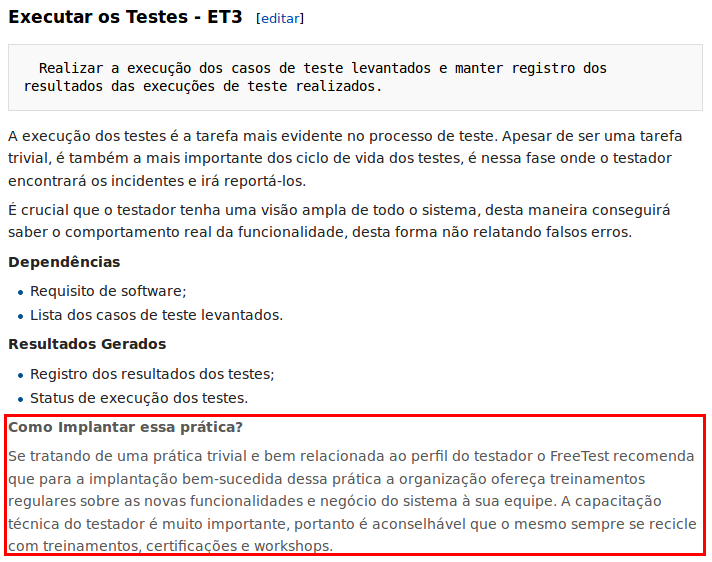
\includegraphics[width=.90\textwidth]{fig/figura51.png}
\caption{Estrutura do guia de implantação: "Como implantar essa prática?"}
\label{fig:fig51}
\end{figure}

A seguir nas próximas subseções podem ser vistos as instruções/sugestões de como implantar todas as práticas especificas sugeridas pelo FreeTest.

\subsection{Realizar análise de risco e definir estratégia de teste – GPT1}
\label{sec:guiagpt1}

Para realização de uma análise de riscos eficiente e definição de qual será a melhor estratégia de teste a ser utilizada é importante que a organização tenha uma documentação de testes mais completa possível. O Método FreeTest não indica um método ou ferramenta específica para levantamento e análise dos riscos, contudo orienta com algumas instruções que podem ser seguidas para que a organização consiga realizar uma análise de risco adequada aos projetos de teste. Uma das formas de se fazer uma análise de risco assertiva é respondendo as seguintes perguntas aos possíveis riscos \cite{Rios}:

\begin{itemize}
\item O risco é relevante para as atividades de teste?
\item Este risco está na alçada de responsabilidades da equipe de testes?
\item O risco é previsível porém não existe nenhuma certeza quanto a sua ocorrência futura?
\item O risco é significante para o projeto de testes?
\item O risco não está sendo tratado pelo plano de gerência de projeto de software?
\end{itemize}

Se a resposta para as perguntas acima foi um "Sim", os riscos devem ser registrados com as seguintes informações:

\begin{itemize}
\item Risco;
\item Tipo de Risco;
\item Probabilidade;
\item Impacto ou Criticidade;
\end{itemize}

\textbf{Sendo que:}

Risco, deve conter a uma descrição do risco em si. É importante que ela seja o mais detalhada possível, pois essa informação servirá como base para os futuros planos de teste.

Tipo de Risco, se tratando de riscos do produto, os riscos podem ser funcionais ou não funcionais neste último caso podem ser categorizados como: usabilidade, acessibilidade, segurança, performance, escalabilidade e segurança.

Probabilidade, é a chance de que o risco ocorra. A sugestão é que seja entre 10\% e 90\% e seja incrementado de 10 em 10. Sendo 0\% a probabilidade não precisa ser tratado, pois não terá chance de ocorrer e 100\% não será um risco e sim um problema já previsto.

Impacto ou Criticidade, a dica é que seja definida a criticidade com um ranking numa escala de 1 a 5, sendo:

\begin{itemize}
\item Impacto baixo no sucesso do projeto;
\item Impacto médio no sucesso do projeto;
\item Impacto alto no sucesso do projeto;
\item Impacto muito alto no sucesso do projeto;
\item Impacto que pode afetar seriamente o sucesso do projeto.
\end{itemize}

É importante que no planejamento dos riscos no ciclo de testes toda a equipe monitore os riscos com maior probabilidade e impacto. Para tanto, pode-se criar uma matriz de Probabilidade versus Impacto, multiplicando as probabilidades pelos Impactos, neste caso obtendo números entre 0,1 (10\% vezes 1) e 4,5 (90\% vezes 5). Pelo bom senso aconselha-se que a equipe monitore todos os riscos altos, ou seja, acima de 4.

Munido de todos os riscos mais relevantes, a equipe pode ter uma visão mais clara de quais riscos monitorar, caso tenha-se um número significante de riscos pode-se definir os TOP-10 maiores, utilizando a tabela mencionada anteriormente. Uma vez com os riscos definidos a equipe pode determinar qual a melhor estratégia tomar para a execução do projeto de teste.

A estratégia de teste por sua vez deverá ser cuidadosamente discutida, pois será peça chave para o sucesso do projeto. A estratégia de teste será fundamentada no escopo do projeto de testes e na análise de risco. Fazem parte da estratégia de teste os seguintes itens:

\begin{itemize}
\item Tipos de Teste que serão executados;
\item Automação dos testes e abordagens;
\item Testes de regressão ou não;
\item Técnicas de teste especifica para algum cenário peculiar.
\end{itemize}

Por fim, é muito importante que a equipe ou gestor mantenha todas essas informações bem documentadas. Outra prática recomendada é a criação de planos de contingência e mitigação dos riscos, utilizados sempre quando um risco se transformar em um problema e para reduzir a probabilidade de incidência do risco, respectivamente.

É importante que tais informações sejam sempre utilizadas como lições aprendidas e que sejam aproveitadas em outros projetos.

\subsection{Definir Escopo de Trabalho para o Projeto – GPT2}
\label{sec:guiagpt2}

O FreeTest recomenda como implantação desta prática específica a criação da Estrutura Analítica do Projeto (EAP), como uma técnica para subdivisão das entregas e do trabalho do projeto em componentes menores e que permitirão o gerenciamento mais fácil.

Por definição uma EAP, segundo o PMBOK \cite{GuiaPMBOK} é um recurso que tem como principal objetivo a divisão do projeto em partes menores (também chamadas de tarefas ou pacotes de trabalho). Consequentemente, estas partes se tornam mais fáceis de serem compreendidas pelos membros da equipe e gerenciadas pelo gestor do projeto.

O FreeTest recomenda as seguintes dicas para criação de uma EAP:

\begin{itemize}
	\item Decomponha a EAP em fases e atividades em níveis, que sejam fáceis de serem gerenciados;
	\item Planeje as entregas, não as ações. Neste caso serão os entregáveis do projeto, quando o mesmo é divido em entregas parciais ao seu cliente;
	\item Quebre os pacotes de trabalho em durações adequadas;
	\item Utilize modelos de EAP de projetos já finalizados. É importante a utilização da base histórica e das lições aprendidas em projetos anteriores.
\end{itemize}

\subsection{Estabelecer estimativas de tempo para realização de tarefas, criação de artefatos e preparação dos ambientes de trabalho – GPT3}
\label{sec:guiagpt3}

A escolha de qual método de estimativa utilizar está muito ligado ao perfil da organização. Normalmente a mesma técnica de estimativa é utilizada por toda a equipe, seja ela de desenvolvimento ou de teste. O FreeTest no entanto, indica algumas técnicas já consagradas, utilizados por equipes ágeis e tradicionais. Abaixo as técnicas recomendadas e como implantá-las na sua organização.

\textbf{Planning Poker}\cite{Cohn2005} O \textit{Planning Poker} ou \textit{Scrum Poke}r tem o propósito de se obter a estimativa por meio de um jogo de cartas, deve permitir que todos os membros da equipe de forma heterogênea participem colocando a sua visão de complexidade, considerando o fator tempo e esforço para pontuar uma carta e após juntos chegar a um denominador comum na equipe através de consenso.

\textbf{Como Implantar o Planning Poker:}
\begin{itemize}
    \item O requisito/\textit{user story} é apresentado inicialmente a toda equipe. É interessante que o mesmo seja feito da forma mais clara e que o entendimento do mesmo seja geral. Neste momento a importância da aceitação do requisito é discutida (pelo \textit{Product Owner});
    \item Cada membro decide individualmente quantos \textit{Story Points} (valores abstratos que representam o tamanho, normalmente convertidos em horas) e seleciona a carta do seu baralho, sem mostrar aos demais;
    \item Quando todos os membros já estiverem com a carta escolhida em mãos, todos viram as cartas ao mesmo tempo;
    \item Caso haja uma discrepância muito grande nos valores, cada um apresenta uma justificativa. Normalmente quem tirou o valor mais alto ao mais baixo;
    \item Depois o time vota novamente até que o grupo chegue a um acordo.
\end{itemize}

\textbf{Estimativa de três pontos} – A estimativa de 3 pontos é uma técnica que permite refinar as estimativas considerando as incertezas e riscos. O conceito origina-se da Técnica de Revisão e Avaliação de Programa (PERT). Segundo o PMBOK, “Uma técnica que usa três estimativas de custos ou duração para representar os cenários otimista, mais provável e pessimista. Esta técnica é aplicada para melhorar a exatidão das estimativas de custos ou duração quando não há certeza em relação à atividade subjacente ou ao componente de custo.”

\begin{itemize}
    \item Com os requisitos já levantados e divididos em pacotes de trabalho deve-se apresentá-los a toda a equipe;
    \item A equipe e/ou gerente de projetos solicita a estimativa para cada tarefa;
    \item O analista deverá definir o tempo otimista (o menor tempo para realizar a tarefa), provável (o tempo convencional) e o pessimista (o maior tempo possível para realizar a tarefa);
    \item Ao final encontra-se a média ponderada somando a estimativa pessimista, mais provável (multiplicado pela constante 4, certificando mais peso para essa variável) e otimista, em seguida o resultado é dividido por 6. O resultado dessa média será então a estimativa gerada pela técnica
\end{itemize}

É importante salientar que a escolha da técnica de estimativa está fortemente ligada à preferência da organização. O FreeTest recomenda as técnicas descriminadas acima, contudo não se opõe ao uso de outras técnicas e até mesmo incentiva a combinação entre técnicas diferentes.

\subsection{Planejar os recursos humanos - GPT4}
\label{sec:guiagpt4}

Uma boa maneira de planejar os recursos humanos ideais para as atividades específicas do projeto de teste é mantendo uma base de currículo de todos os integrantes da equipe. Tal prática apesar de trivial é pouco feita pelas organizações. O FreeTest ainda reforça que a gestão dessa base de currículo não seja simplesmente um arquivo com certificados e diplomas, mas sim um repositório com todas as informações mais atualizadas da equipe, contendo conhecimentos adquiridos durante os projetos, workshops ministrados e assistidos.

O FreeTest salienta também a importância de treinamentos recorrentes nas equipes. Em pequenas organizações onde o time é mais enxuto e heterogêneo é interessante que se faça com frequência workshops para disseminação de conhecimento. Essa prática além de promover o espírito colaborativo da equipe tornará o conhecimento tácito em explícito ajudando assim a gestão de conhecimento da organização.

\subsection{Determinar e documentar os riscos do projeto de teste, assim como seu impacto, probabilidade de ocorrência e prioridade de tratamento - GPT5}
\label{sec:guiagpt5}

Uma técnica simples que atende essa prática é a realização de brainstormings com a intenção de obter uma lista completa dos riscos do projeto. O interessante é que toda a equipe participe, desta maneira uma equipe multidisciplinar tem mais chances de identificar, documentar, categorizar e criar planos de mitigação dos riscos.

É importante que todos os resultados encontrados durante as reuniões de brainstorming sejam mantidos em uma base de dados, acompanhado de todas as informações inerentes ao risco, como impacto, probabilidade de ocorrência e planos de mitigação e resposta ao risco.

\subsection{Monitorar o progresso do projeto com relação ao estabelecido no planejamento e assessorar na realização de pendência - GPT6}
\label{sec:guiagpt6}

O monitoramento normalmente é feito por ferramentas de controle de projetos, no qual é possível avaliar o status e progresso das atividades. Uma técnica recomendada é a utilização de reuniões para acompanhamento do projeto com certa frequência, é possível, por exemplo manter uma rotina de reuniões diárias para que a equipe repasse o feedback das atividades e que ressalte qualquer problema ocorrido.

\subsection{Identificar Casos de Teste – ET1}
\label{sec:guiaet1}

Casos de teste podem ser identificados de diversas maneiras e descritos utilizando diversos métodos, desde descrições visuais como, mapas mentais à descrições textuais que são as mais comuns. A implantação dessa prática está ligada às preferências e tecnologias da organização, no entanto o FreeTest mostra algumas formas para identificação e documentação de casos de teste. As técnicas principais para a identificação e criação de casos de teste seguem abaixo:

\begin{itemize}
    \item \textbf{Particionamento por Classe de Equivalência} – O objetivo dessa técnica é eliminar os casos de testes redundantes dividindo as entradas de dados em classes de equivalência que serão testadas no lugar de toda a entrada. A criação de casos de teste para particionamento de equivalência é baseado numa avaliação das classes de equivalência para uma condição de entrada. ;
    \item \textbf{Análise de Valor Limite} - São casos de teste que exploram limites dos valores de entrada, neste caso tem mais probabilidade de encontrar defeitos. Os valores são escolhidos imediatamente acima ou abaixo dos limites definidos nas classes de equivalência.
\end{itemize}

Abaixo algumas dicas que podem ser seguidas para identificação de casos de teste, o FreeTest recomenda a utilização das técnicas já mencionada acima em combinação das instruções mostradas a seguir:

\begin{itemize}
    \item Utilize a documentação do software/negócio mais atualizada, caso não tenha documentação necessária, em linhas gerais defina o que deverá ser testado;
    \item Caso tenha documentação, como casos de uso, pode ser feito a derivação dos casos de teste a partir de sua estrutura padrão, utilizando basicamente dois métodos, derivação textual e visual
    \item \textbf{Derivação textual}: Sendo que para a derivação textual cada caminho deve ser mapeado, pois de cada caminho será extraído um requisito de teste.
    \item \textbf{Derivação visual}: Todo o caso de uso tem um desenho de todos os fluxos de eventos juntos, que pode ser usado como base na derivação visual;
    \item Se o sistema possui telas com muitos campos e com muitas probabilidades de situações, tais como regras de negócio, faça as combinações que você acha pertinentes em função das regras que seu teste pede. Neste caso é aconselhável usar teste por \textbf{tabela de decisões} se o nível de complexidade for alto ou médio;
    \item Use sempre técnicas como valor limite e particionamento por equivalência para reduzir e ser mais assertivo com seus casos de teste;
    \item Criar casos de teste para diversas situações em ambientes distintos, como banco de dados, resoluções de tela, plataformas e outros.
\end{itemize}

A criação de ambientes como mencionado anteriormente é inerente a forma de como a organização trabalha. No entanto, o FreeTest aconselha fortemente a criação de ambientes virtualizados, pois além de mais versáteis, menor custo é possível realizar o seu versionamento. Através do versionamento de ambientes é possível realizar rollbacks do ambiente de forma mais ágil e flexível. Essa agilidade e flexibilidade na criação de ambientes torna as tarefas corriqueiras mais fáceis de serem realizadas, dessa forma fluindo melhor o processo e cumprindo melhor os prazos do projeto.

\subsection{Criar/Atualizar Ambiente de Teste - ET2}
\label{sec:guiaet2}

A criação de ambientes como mencionado anteriormente é inerente a forma de como a organização trabalha. No entanto, o FreeTest aconselha fortemente a criação de ambientes virtualizados, pois além de mais versáteis, menor custo é possível realizar o seu versionamento. Através do versionamento de ambientes é possível realizar rollbacks do ambiente de forma mais ágil e flexível. Essa agilidade e flexibilidade na criação de ambientes torna as tarefas corriqueiras mais fáceis de serem realizadas, dessa forma fluindo melhor o processo e cumprindo melhor os prazos do projeto.


\subsection{Executar os Testes - ET3}
\label{sec:guiaet3}

Se tratando de uma prática trivial e bem relacionada ao perfil do testador o FreeTest recomenda que para a implantação bem-sucedida dessa prática a organização ofereça treinamentos regulares sobre as novas funcionalidades e negócio do sistema à sua equipe. A capacitação técnica do testador é muito importante, portanto é aconselhável que o mesmo sempre se recicle com treinamentos, certificações e workshops.

\subsection{Reportar e Acompanhar Incidentes - ET4}
\label{sec:guiaet4}

Não existe uma maneira “mais correta” de reportar um incidente, contudo seguem algumas informações importantes que se deve ter no relato de um incidente:

\begin{itemize}
    \item Prover aos desenvolvedores e outros envolvidos um retorno sobre o problema para permitir a identificação, isolamento e correção se necessário;
    \item Prover aos lideres de teste um meio para se rastrear a qualidade do sistema em teste e o progresso do teste;
    \item Prover ideias para aprimorar o processo de testes. Os detalhes de um relatório de incidente podem incluir: Data da emissão, autor, status e organização;
    \item Resultados esperados e resultados atuais;
    \item Identificação do item de teste (item de configuração) e ambiente;
    \item Processo do ciclo de vida do sistema ou software em que o incidente foi descoberto;
    \item Descrição do incidente para permitir a reprodução e resolução, incluindo logs, database dumbs, ou screenshots;
    \item Escopo e grau de impacto para os stakeholder;
    \item Severidade do impacto no sistema;
    \item Urgência / Prioridade na correção;
    \item Estado (status) do incidente (aberto, rejeitado, duplicado, aguardando resolução, aguardando reteste ou fechado);
    \item Conclusão, recomendações e aprovações;
    \item Comentários gerais, tais como outras áreas que podem ser afetadas por uma mudança resultante de um incidente;
    \item Histórico de mudanças, como a sequência de ações tomadas pela equipe envolvida no projeto com respeito ao isolamento do incidente, reparo e confirmação da resolução;
    \item Referências, incluindo a identificação da especificação do caso de teste que revelou o problema;
    \item A estrutura de um relatório de incidente pode ser encontrada no “Standard for Software Test Documentation” (IEEE Std. 829-1998).
\end{itemize}

\subsection{Encerrar teste - ET5}
\label{sec:guiaet5}

O FreeTest recomenda o uso de uma base de conhecimento para manutenção das informações importantes coletadas durante todo o ciclo de vida do projeto e ao término dele. Essas informações históricas, mantidas em um local apropriado guiará os próximos projetos a planejamentos mais assertivos e projetos menos suscetíveis a erros.

O uso de ferramentas para manutenção da base histórica é altamente recomendado. Pode-se ainda incluir relatos de acontecimentos peculiares ao projeto, informações sobre fatos que geraram algum transtorno e como resolvê-los, por exemplo, informações sobre dependências de bibliotecas de terceiros, configurações de ambientes e etc.

\subsection{Realizar verificação - RR1}
\label{sec:guiarr1}

O FreeTest recomenda que as revisões aconteçam de forma intercalada quando forem realizadas por profissionais que desempenham o papel de analista de requisitos e teste, e quando os papéis de analista requisito e teste forem feitos por pessoas diferentes a sugestão é que o testador que for fazer a revisão do requisito seja o mesmo que for testar o software. Desta maneira o testador estará munido de mais informações sobre os requisitos.

É Fundamental fazer um checklist com os principais erros e pontos relevantes. A criação de um checkllist pode direcionar as revisões, tornando mais fácil e prático as sessões de revisão dos requisitos. A criação do checklist vai de acordo com as necessidades da organização, geralmente voltado para os erros mais comuns cometidos.

\subsection{Relatar e Acompanhar Inconsistências - RR2}
\label{sec:guiarr2}

O relato das inconsistências pode ser realizado utilizando uma ferramenta de bug tracker ou até mesmo inserindo comentários no texto revisado.

\subsection{Encerrar verificação - RR3}
\label{sec:guiarr3}

Aconselha o uso de uma ferramenta para o relato das inconsistências encontradas. As mesmas serão mantidas a título de base histórica para melhoramento continuo das atividades.

\subsection{Criar/Atualizar ambiente de teste - TDA1}
\label{sec:guiatda1}

A recomendação mais importante é que o ambiente de testes seja mais fiel ao ambiente de produção, pois assim, problemas relacionados com ambientes serão evidenciados durante os testes de aceite. O teste de aceitação é uma atividade muito importante para a entrega do software com qualidade e valor ao cliente, portante é importante que o mesmo seja feito de forma adequada e simulando aspectos e comportamentos que o ambiente do cliente proporciona.

\subsection{Executar teste de aceite - TDA2}
\label{sec:guiatda2}

O teste de aceitação tem como objetivo confirmar se o sistema está funcionando conforme o esperado, ou seja, prover a confiabilidade de que esteja de acordo com o requisito. Outro objetivo é avaliar se a qualidade do software, para prover informações sobre os riscos da implantação do sistema em um determinado momento aos gestores. Enfim, o objetivo principal do teste de aceitação não é encontrar defeitos e sim garantir a entrega de valor para o cliente.

\subsection{Encerrar teste de aceite - TDA3}
\label{sec:guiatda3}

Aconselha o uso de uma ferramenta para o relato das inconsistências encontradas. As mesmas serão mantidas a título de base histórica para melhoramento continuo das atividades.
Identificar produtos de trabalho, tipos e critérios de revisão - AES1
O ideal é que a organização realize a análise estática de código e revisão em pares de todo o código fonte possível. O critério de escolha para realização das revisões está muito relacionado ao perfil da equipe e efetivo de pessoas.
A revisão em pares por ser uma prática mais “cara” pode ser reduzida a partes específicas do código, geralmente partes mais críticas e que contem mais lógicas de negócio. Outra maneira efetiva de escolher o que revisar é indicando analistas seniores para realizar o levantamento das áreas críticas do sistema, geralmente onde há muita dependência entre códigos fontes e/ou há muita regra de negócio.
O FreeTest recomenda o uso de checklists de “boas práticas” contendo os critérios de revisão para orientar as sessões de revisão. Esse checklist é importante, pois guiará mais facilmente as revisões, principalmente quando o revisor não conhece bem os critérios usados para a revisão de código da organização.

\textbf{Identificar produtos de trabalho, tipos e critérios de revisão - AES1}

O FreeTest recomenda que o código escrito por um desenvolvedor, antes de ser enviado para o ambiente de produção, seja revisado por outro membro da equipe. Essas revisões podem ser feitas de diversas maneiras, como, por exemplo, programação em pares, ou mesmo realizando uma leitura/revisão sistemática do código. Após a revisão o revisor destaca todos as inconsistências encontrados e envia ao autor original do código. O autor do código avalia os comentários recebidos e eventualmente realiza as correções no código-fonte.
Uma boa dica para realizar a revisão é que desenvolvedores mais seniores o façam, pois como conhecem mais o software e regras de negócio poderão facilmente encontrar inconformidades e orientar os demais membros da equipe para as eventuais correções.
A melhor forma de se implantar essa prática é utilizando ferramentas de versionamento de código. É possível através delas inserir comentários nos códigos/artefatos e solicitar que demais membros da equipe façam as correções. É interessante também utilizar esses ambientes para definir os critérios de aceite das revisões, por exemplo, o código só será aceito (entrará em produção) se for analisado por mais de dois desenvolvedores e que um deles seja sênior.

\subsection{Conduzir revisão de Código - AES2}

A análise estática de código feita de forma automática depende basicamente de ferramentas. A escolha da ferramenta é algo muito inerente a Organização e está relacionada as tecnologias utilizadas. A escolha correta das ferramentas ajudarão a equipe a encontrar inconsistências precoces referentes às regras de estilo e erros comuns.
Para implantação dessa prática a equipe pode definir em processo que essa tarefa entra como um critério de qualidade da organização, sendo necessário que toda vez que um código fonte for desenvolvido ele deverá passar pelas ferramentas de Análise Estática. O FreeTest disponibiliza uma lista de ferramentas para o uso dessa prática, contudo o uso e implantação da mesma é responsabilidade da Organização. Segue uma lista de

\subsection{Definir critérios para seleção de casos de teste para automação - AET1}

Como já mencionado anteriormente quanto maior a automatização dos casos de teste, melhor. No entanto, quando não é possível automatizar todos os cenários é essencial que se tenha um critério de seleção para quais casos de teste automatizar. O critério de escolha está muito ligado às regras de negócio do produto, cliente e particularidades do projeto, tecnologias e etc. Todavia o FreeTest recomenda algumas práticas a serem tomadas para facilitar a escolha dos casos de teste passíveis de automação.

\subsection{Definir um framework para automação de teste - AET2}

A escolha do aparato técnico necessário para se implementar um ambiente automatizado está ligado, principalmente às tecnologias e recursos da organização. O FreeTest recomenda o uso de algumas ferramentas amplamente utilizadas no mercado, no entanto a escolha de qual ferramenta utilizar é de decisão final da empresa. Todavia recomendamos alguns critérios a serem analisados na escolha:

\begin{itemize}
\item Usabilidade – A grande distinção entre as ferramentas de automação com relação a sua usabilidade está se a mesma disponibiliza uma interface/IDE para criação dos scripts de forma mais alto nível ou se, somente é possível a escrita de scripts diretamente.
\item Expertise da equipe – A ferramenta a ser escolhida é conhecida por algum membro da equipe? Caso não haja um conhecimento na ferramenta poderá ser investido tempo/dinheiro na aprendizagem da mesma.
\item Suporte – O suporte da ferramenta é algo importante. Mesmo sendo uma ferramenta open-source é importante se a comunidade mantém uma rede que dá suporte a ferramenta, se existem fóruns especializados de ajuda, ou até mesmo, criação de plugins.
\item Tecnologia e propósito especifico – Ferramentas podem atender propósitos específicos, como performance, segurança, carga e etc, então é bom alinhar a escolha da ferramenta com a necessidade da organização. Outro fator trivial à análise do framework de automação é com relação a linguagem de programação que a mesma atende, ou seja, Java, Python, C etc.
\end{itemize}

\subsection{Gerenciar incidentes de teste automatizado - AET3}

Essa atividade é importante, se tratando principalmente de empresas com um baixo nível de maturidade com o processo de automação de testes. No incio a infraestrutura de automação é prematura e muitos erros e ausências de validações podem ocorrer, pensando nisso é importante que haja um controle mais rigoroso sobre os erros evidenciados pela arquitetura de automação.
No entanto, se tratando de erros encontrados é muito importante que a própria arquitetura de automação faça os relatos dos erros de forma automática, na verdade esse é um resultado comum de várias ferramentas no mercado. Contudo caso a arquitetura seja criada a partir do zero, como é o caso de organizações que optam por usar tecnologias \textit{open-source}, seguem algumas informações importantes para que o relato das inconsistências sejam efetivos.

\subsection{Automatizar a execução dos testes Automatizados - AET4}

A melhor maneira de implantar essa prática é dispor de ferramentas de automatização de tarefas e integração entre as mesmas, neste caso ferramentas de Integração Contínua. O FreeTest recomenda o uso de algumas ferramentas, no entanto, não se limita a elas. Essa prática normalmente é transversal a todas as áreas do ciclo de desenvolvimento de software, não somente ao teste, e deve ser encorajada para as demais áreas, para que se tenha o máximo de aproveitamento desse tipo de prática de trabalho.

\subsection{Versionar Artefatos/scripts/planos/infraestrutura de Teste - GCT1}

A Gerência de Configuração só é factível com o uso de ferramentas de versionamento. O FreeTest indica o uso de algumas ferramentas, no entanto, quais artefatos versionar é relativo as necessidades da organização. Como já mencionado indicamos o versionamento dos artefatos básicos de projeto de teste, scripts de automação e quando a organização utiliza a infraestrutura como serviço é interessante que haja o versionamento dos ambientes base.

\subsection{Criar baseline dos artefatos/scripts/planos já testados - GCT2}

Uma boa prática para criação das baselines é alinhar as nomenclaturas e padrões utilizados na etapa de desenvolvimento. Então neste caso, caso seja gerado no desenvolvimento a versão 1.1 do software onde contemplará todo o código fonte e artefatos relacionados ao desenvolvimento, na etapa de teste todos os artefatos e scripts de teste também deverão ser versionados e definidos uma baseline ao final de cada etapa.

Com o uso de ferramentas apropriadas para a criação e versionamento dos ambientes de teste pode-se definir uma rotina de versionamento, ou seja, de tempos em tempos os ambientes serão versionados. Os ambientes podem ser versionados antes do início dos testes, para garantir uma cópia padrão com aquela versão do software e após o encerramento dos testes, contendo uma versão final do software.

\subsection{Definir Objetivos de Medição de Teste - MED1}

A melhor maneira de definir quais objetivos de teste usar é buscar as necessidades de informação da organização. Em organizações menores geralmente é muito importante conhecimento sobre efetividade dos testes e quantidade de bugs encontrados nos clientes, o FreeTest indica algumas métricas que podem ser utilizadas para medição:

\begin{itemize}
\item Quantidade de Bugs Encontrados;
\item Medir cobertura de testes;
\item Quantificar erros encontrados no cliente;
\item Efetividade dos testes;
\item Tempo planejado versus tempo executado de atividades;
\item Feedback de cliente (pós implantação).
\end{itemize}

\subsection{Coletar, analisar e comunicar dados de medição - MED2}

Uma coleta efetiva de métricas está atrelada às informações que essa organização gera e os objetivos de medição que ela define. Neste caso é importante sempre coletar e analisar métricas que são possíveis de se extrair resultados efetivos para a organização. A escolha da melhor técnica para análise dos dados coletados para medição vai de encontro aos objetivos que a organização definiu. No entanto, o FreeTest recomenda alguns métodos já conhecidos na literatura.

\subsection{Armazenar dados de medição - MED3}

O armazenamento das medições deve ser realizado sempre ao final da sua coleta com a finalidade de garantir base histórica e informações de desempenho do projeto de teste. Uma rotina importante a ser feita sempre que necessário consolidar e armazenar as medições são as seguintes:

\begin{itemize}
\item Revisão dos dados coletados;
\item Utilizar o padrão organizacional de armazenamento das informações;
\item Disponibilizar o acesso as informações somente a equipe apropriada;
\end{itemize}

\subsection{Gerar build Automatizado - INC1}

Considerando que o ambiente de integração contínua já está em ativo funcionamento é interessante que se determine uma nomenclatura para a geração das builds e que a mesma seja feita de forma automática. É interessante que plugins de comunicação sejam instalados para o envio de e-mail na equipe, desta forma, toda vez que um build for gerado os interessados serão comunicados.

O procedimento básico para criação de builds e aconselhado pelo Freetest baseia-se nos seguintes passos:

\begin{itemize}
    \item O desenvolvedor implementa o código (seja uma correção, melhoria ou novo código);
    \item Realiza os testes caixa branca e revisões de código necessárias;
    \item Envia o código para sua branch no repositório principal;
    \item Notifica os interessados, neste caso os testadores também;
    \item Por sua vez o testador gera o build através da integração contínua;
    \item Finalmente os testes são realizados e os erros relatados.
\end{itemize}

Perceba que além da automatização de uma tarefa recorrente, que é a geração do build, a equipe ganha com feedback automático e obviamente com tempo. Algumas recomendações importantes podem ser seguidas para a geração de builds em ambientes de Integração Continua:

\begin{itemize}
	\item Focar no desenvolvimento de pequenas alterações do que em grandes alterações no código. Quando for necessário alterar uma grande parte do código, desmembrá-la o máximo possível;
	\item Criar uma massa de testes abrangente. Construa essa massa de teste, pouco a pouco, não é necessário escrever testes para todo o código em um único dia.
	\item Automação máxima do pipeline (testes estáticos, cobertura, unitários);
	\item Usar técnicas para geração de \textit{releases} mais enxutas, como \textit{Toggles} e \textit{Canary} \textit{releases}. É uma boa medida para entregar novas funcionalidades do software de maneira mais segura e gradual.
\end{itemize}

\subsection{Executar análise estática automatizada - INC2}

A análise estática de código automatizada visa evidenciar problemas triviais (ou não) inseridos no código fonte. A Automatização desta atividade é amplamente recomendada, principalmente dentro de um ambiente de Integração Contínua, por ser uma atividade corriqueira e facilmente automatizada. 

A implantação desta prática envolve muito o aparato técnico e de infraestrutura da organização. Desta forma é muito importante que integrantes mais seniores e técnicos façam parte da implantação desta prática, pois devera realizar a escolha de ferramentas de acordo com o código fonte do software desenvolvido, por exemplo. O estudo "Estudo, Definição e Implementação de um Sistema de Recomendação para Priorizar os Avisos Gerados por Ferramentas de Análise Estática" \cite{estudoDefinicaoAnalisEstatica} fornece uma base de conhecimento sobre algumas ferramentas, e pode auxiliar na implantação desta prática.

\subsection{Executar conjunto de testes automatizados abrangentes - INC3}

A execução dos testes abrangentes em um ambiente de Integração Continua é importante, pois cria um "filtro" a mais para evidenciar bugs ou possíveis bugs. Como se trata de um ambiente automatizado de uma atividade repetitiva e que ocorre bem próximo ao desenvolvimento, entende-se que é uma prática eficaz na a melhoria continua do código-fonte.

Essa prática auxilia o testador a identificar possíveis "lacunas" a serem melhoradas na cobertura do código fonte. Por se tratar de uma execução automatizada dos testes abrangentes o testador com base no resultado da execução, poderá auxiliar o desenvolvedor antes mesmo da geração do build a melhorar a cobertura do código fonte e sanar possíveis problemas. No ponto de vista da equipe de testes essa atividade pode auxiliar no aprendizado mútuo, da resolução do problema, redução de ruídos na comunicação, no entendimento do negócio por parte do testador e, por fim, engajamento da equipe.

Abaixo uma lista de algumas características que poderão ser criados testes automatizados, e que neste caso, é imprescindível o apoio/realização da tarefa por parte do testador.

\begin{itemize}
    \item Conciso;
    \item Repetitivo;
    \item Limpo;
    \item Eficiente;
    \item Independente;
    \item Sustentável.
\end{itemize}

\subsection{Executar criação de ambientes virtualizados de forma automatizada - INC4}

Em adicional à qualidade dos testes, é também importante ter cuidado com os ambientes onde os mesmos serão gerados. Algumas recomendações gerais são aconselhadas pelo FreeTest:

\begin{itemize}
	\item "Ambientes Limpos": É de suma importante que os testes sejam executados em ambientes limpos, ou seja, não sofram interferência de outras baterias de testes realizadas anteriormente. Se tratando de ambientes de IC que integram com práticas DevOps é possível usar mecanismos de provisionamento para gerar ambientes limpos toda vez antes da execução dos testes. Organizações que usam do conceito de Infraestrutura como Serviço, podem gozar dessa possibilidade sempre criando \textit{snapshots} de seus ambientes.
	\item Fidelidade: Ambientes de teste devem ser o mais fieis possível do ambiente de produção. Pode-se então clonar ambientes de produção limpos e sempre usá-los para testes.
	\item Ambientes Baratos e Flexíveis: Infraestrutura como um todo é sempre um custo alto para organizações. Desta forma pensar em ambientes virtualizados e sob-demanda é uma alta alternativa para reduzir custos e melhorar a performance da criação de ambientes de teste, já que é de suma importância que os ambientes de testes possam inicializar/desligar rapidamente e serem flexíveis a mudanças.
\end{itemize}

\subsection{Preparar massa de teste - TRG1}

Tipicamente dados de teste devem ser gerados antes do inicio da execução dos testes, isto porque é difícil realizar essa tarefa durante o gerenciamento dos dados. Isso por que essa etapa para geração dos dados de teste consome muito tempo, então é importante que seja feita antes da execução dos testes de regressão, pois pode atrapalhar a deadline para execução desta atividade. Para cada modalidade de teste (Testes Caixa Branca, Segurança, etc) existem várias boas práticas que podem ser seguidas, no entanto para Teste de Regressão o FreeTest recomenda algumas:

\begin{itemize}
    \item Sem dado: Sistema deverá validar quando nenhum dado é submetido;
    \item Dado Válido: Verificar se o sistema valida quando um dado correto é inserido;
    \item Dado Inválido: Verificar se o sistema valida quando um dado incorreto é inserido;
    \item Formato Inválido: Verificar resposta do sistema quando um dado com formato inválido é inserido;
    \item Valor Limite: Dados que representam os limites inferiores e superiores do campo;
    \item Particionamento por Equivalências: Criar massa de dados que representam equivalências entre conjuntos;
    \item Tabela de Decisão: Criar massa que representem os dados de uma tabela de decisão.
\end{itemize}

A escolha da melhor técnica para criação da massa de dados depende do cenário de teste. Para cada tipo de modalidade de software e área de atuação as técnicas acima podem ser utilizadas ou combinadas com outras.

\subsection{Manter \textit{scripts} de regressão - TRG2}

As manutenções nos scripts de teste devem ser atividades corriqueiras na organização. Uma vez que o acúmulo dessa atividade pode dificultar a manutenção e/ou comprometer partes íntegras dos mesmos. Recomenda-se que sempre antes de realizar um teste de regressão verificar os \textit{scripts} e massas utilizadas, para que não ocorra quebra no fluxo normal da execução automatizada.

\subsection{Executar teste de regressão - TRG3}

O FreeTest defende a visão de que casos de teste criados durante a produção devem ser automatizadas e armazenadas em um repositório para posterior execução, criando assim, uma lista de casos de testes para regressão. Esta lista para regressão tem o propósito de assegurar que os incidentes encontrados não se repetirão, garantindo a confiabilidade do produto pelo cliente.

Considerando que a geração de builds em times ágeis ocorre com maior frequência é crucial que o time de teste execute suítes de regressão em períodos mais curtos de tempo. Automatizar a execução das suítes de regressão é uma decisão muito interessante, pois como essa modalidade de teste é recorrente e pode ser executada através de um ambiente de Integração Contínua o retorno de investimento é de curto, médio prazo.

	
\subsection{Encerrar teste de regressão - TRG4}

O FreeTest orienta que ao finalizar os testes de regressão deve-se apresentar um relatório da execução dos testes. Esse relatório é uma forma de avaliar a qualidade e criar confiabilidade no produto que está sendo produzido. Mesmo que haja defeitos ainda a serem consertados, o responsável pelo produto tem a exata noção de como anda a qualidade, podendo tomar as devidas ações em casos de desvios da qualidade ou, em casos extremos, abortar a produção do sistema.

Normalmente as ferramentas de automação utilizadas nos testes de regressão disponibilizam relatórios para as análises dos resultados, no entanto é responsabilidade da organização definir quais as métricas e indicadores serão mais adequados às suas necessidades.

\subsection{Preparar ambiente de teste - TPE1}

O ambiente de teste de desempenho deve ser o mais próximo possível do ambiente de produção. Essa tarefa não é fácil e demanda muito conhecimento técnico, as vezes tornando-se uma tarefa que pode demorar dias e até semanas, por isso se faz importante o planejamento desta atividade de forma bem minuciosa.

Essa prática está ligada ao contexto de uso da aplicação, características técnicas e aos objetivos de teste que se desejam alcançar, porém o FreeTest lista alguns desafios que devem ser considerados para essa prática:

\begin{itemize}
	\item Infraestrutura de Servidor: Replicar o ambiente de produção para esse tipo de teste não é fácil. Demanda alto \textit{know-how} técnico, tempo e um custo adicional ao projeto.
	\item Infraestrutura de Rede: Para suportar a quantidade requisições é importante prever que a infraestrutura de rede a ser utilizada nos testes suporte uma grande carga de requisições.
	\item Tamanho do Banco de Dados: O tamanho do banco de dados pode impactar nos testes, desta forma é importante que o banco de dados, além de ser o mesmo utilizado pela produção, seja simulado no mesmo ambiente e de preferência com o mesmo tamanho.
	\item Testes Geograficamente Distintos: É importante simular requisições de diferentes localizações. Para isso existem algumas ferramentas que emulam tal tipo de serviço.
\end{itemize}


\subsection{Manter \textit{script} de desempenho - TPE2}

Os scripts de desempenho devem ser versionados em repositório de teste padrão e mantida uma nomenclatura adequada. Sempre que possível fazer uma rastreabilidade das funcionalidades que deverão sofrer o teste de desempenho com os \textit{scripts} que já foram gravados pra mesma.

Em arquiteturas monolíticas, pode-se criar uma subdivisão e nomenclatura por funcionalidades, enquanto que para arquiteturas \textit{micro services} além dessa divisão, deve-se dividir por cada  serviço.


\subsection{Executar teste de desempenho - TPE3}

Antes de iniciar qualquer modalidade de teste de desempenho é necessário definir o escopo da sua aplicação em termos de desempenho. Alguns parâmetros são definidos abaixo para guiar a Organização nesta definição de abrangência dos testes e objetivos de qualidade a serem alcançados: 

Objetivos de Teste:

\begin{itemize}
	\item Os objetivos de teste devem ser bem específicos e realistas;
	\item Aspectos não funcionais e funcionais devem ser levados em consideração.
\end{itemize}

Aspectos Funcionais:

\begin{itemize}
	\item Carga: número de usuários;
	\item Cobertura Funcional: Escolha de funcionalidades (regra dos 80/20);
	\item Satisfação do usuário: Tempo resposta limite;
\end{itemize}

Parâmetros Técnicos:

\begin{itemize}
	\item Tipo de Arquitetura: Monolítica, \textit{Micro Services} e etc;
	\item Infraestrutura: Aspectos de hardware em geral ou virtualização.
\end{itemize}


Segundo o RUP (\textit{Rational Unified Process}) \cite{RUP940320} o teste de desempenho abrange os seguintes tipos de teste:

\begin{itemize}
	\item Teste de avaliação de desempenho: Compara o desempenho de um objetivo do teste novo ou desconhecido em relação a um padrão de referência conhecido, como softwares ou medições existentes.
    \item Teste de contenção: Verifica se o objetivo do teste pode tratar de forma aceitável as demandas de vários atores no mesmo recurso (registros de dados, memória e assim por diante).
    \item Perfis de desempenho: Verifica a aceitabilidade do comportamento de desempenho do objetivo do teste através de configurações variáveis, enquanto as condições operacionais permanecem constantes.
    \item Teste de carga: Verifica a aceitabilidade do comportamento de desempenho do objetivo do teste em condições operacionais variáveis (como número de usuários, número de transações, etc.), enquanto a configuração permanece constante.
    \item Teste de stress: Verifica a aceitabilidade do comportamento de desempenho do objetivo do teste quando condições anormais ou extremas forem encontradas, como a redução dos recursos ou um número extremamente alto de usuários.
\end{itemize}

\subsection{Encerrar teste de desempenho - TPE4}


Estando os testes de desempenho concluídos, seus resultados deverão ser compilados de forma a identificar os defeitos que eventualmente tenham ocorridos, bem como o plano de ação aplicado para resolução destes. Com isso haverá condições de se obter o nível de qualidade sobre o aspecto de desempenho da software.

O FreeTest aconselha que os resultados gerados sejam versionados e utilizados como lições aprendidas durante o projeto. A disseminação dessas informações dentro da equipe é de suma importância para aumentar o engajamento e trazer confiança para a equipe.


\subsection{Definição da abordagem de automação que será utilizada - TCA1}

A escolha da melhor abordagem para realização dos testes contínuos automatizados é muito inerente às características da Organização. Não só no que diz respeito à linguagem(ens) utilizadas para codificação do software, \textit{know-how} e também limitações financeiras \cite{Castelo2015}.

Há muitos aspectos que devem ser considerados na escolha da melhor abordagem para automação contínua, o FreeTest lista alguns:

\begin{itemize}
	\item Facilidade de Integração: A ferramenta deve integrar facilmente com todo o ecossistema de desenvolvimento. Neste sentido a ferramenta além de ter uma boa performance na execução dos casos de teste, deve ser compatível com a arquitetura, dar suporte à linguagem de programação que a empresa utiliza, ter uma linguagem \textit{script} de fácil entendimento e suporte na internet.
	\item Performance: Como a ferramenta se comporta no ambiente de desenvolvimento com o tráfego de rede e o hardware, por exemplo. A correta avaliação da ferramenta pode possibilitar que a equipe execute testes até mesmo em ambientes virtuais sem nenhum problema.
	\item Tipos de Teste: Tipos de teste que a ferramenta executa, pois dependendo dos tipos de teste que a ferramenta executa não atenderá o cenário da empresa.
	\item Manutenção: Suporte da comunidade online é muito importante. Reduz a curva de conhecimento e feedback mais rápido para resolução de problemas e auxílio em dúvidas.
	\item Custo: Automação por si só possui um custo elevado e mão de obra mais restrita, desta forma é bom analisar o custo de uma ferramenta antes da sua implantação.
	\item \textit{Cross Browser} / \textit{Headless Browse}r: No contexto dos testes funcionais/testes de aceitação é muito importante validar se a ferramenta desejada suporta tecnologias \textit{Cross Browser}, que realiza os testes na tela ou se realiza os testes utilizando DOM do navegador, sem uma interface gráfica, somente requisições (\textit{Headless Browser}).
\end{itemize}


\subsection{Automatizar \textit{suites} de teste contínuos - TCA2}

Testes Contínuos Automatizados envolvem uma séries de modalidades de teste, como técnicas, funcionais, performance, unidade, aceitação/integração e etc. O FreeTest recomenda que pelo menos a \textit{suite} de testes de aceitação e unidade sejam integrados ao \textit{pipeline} de teste. Outro fator de sucesso para a implantação desta prática é que a Organização precisa estar alinhada com uma mentalidade mais "agilista" e ter em mente que:

\begin{itemize}
	\item Os testes devem ser contínuos e devem ter seu espaço dentro do desenvolvimento do software;
	\item Os ambientes de teste/produção devem ser executados automaticamente e de forma rápida;
	\item Deve existir o máximo de cobertura de código;
	\item Os dados de teste devem ser gerados sob demanda e num formato que atenda a execução dos casos de teste;
	\item O software deve ter uma usabilidade permitindo que a equipe esteja familiarizada em pouco tempo;
\end{itemize}

\textbf{Automatizando Testes de Aceitação:}

A \textit{suite} de testes de aceitação será executada a cada novo \textit{build} gerado com a intenção de validar se o \textit{build} é "testável" e então ser enviado para a equipe de teste. O teste de aceitação faz uma cobertura mais abrangente do \textit{build}, não tem a intenção ser minucioso/preciso. Estes casos de teste geralmente são o "\textit{core}" do sistema e quando executados e falhos retornam para o desenvolvedor para que sejam corrigidos, antes de enviar para a equipe de teste, evitando assim a entrega de builds instáveis para a equipe.

Os \textit{scripts} criados para o teste de aceitação costumam avaliar primeiro a estabilidade da \textit{build} e então validam as integrações entre os códigos e por fim o funcionamento correto das funcionalidades a serem testadas. Essa prática é importante, pois é muito comum que as equipes trabalhem separadamente no mesmo módulo dos sistema. Todos os casos de teste criados devem ter resultados esperados, não é aconselhável mesclar códigos de módulos "instáveis", ou seja, não concluídos totalmente e é altamente recomendado que se tenha uma cobertura de teste o suficiente para abranger as funcionalidades mais críticas.

Como automatizar todos os cenários possíveis para aceitação nem sempre é viável, aconselha-se que fazer um levantamento das funcionalidades mais críticas e principais do ponto de vista do negócio, então gravar os \textit{scripts} de aceitação. Em um ambiente de Testes Contínuos a execução dos \textit{scripts} de aceitação ocorrem normalmente dentro do ambiente de Integração Contínua e são executados logo após a geração do \textit{build}, os passos podem ser vistos a seguir:

\begin{itemize}
	\item Resultados dos testes de aceitação referente ao \textit{build} gerado;
	\item Desenvolvedor responsável pelo \textit{build} análise os resultados;
	\item Se houve falha no \textit{build} o responsável diagnostica a causa da falha;
	\item Se a falha for relativa à um \textit{bug}, todos os dados relacionados ao erro são enviados para o desenvolvedor responsável;
	\item O desenvolvedor responsável corrige o erro;
	\item Após as correções o \textit{build} é novamente gerado e a suíte de testes executadas novamente até que todos os casos de testes passem e o \textit{build} estável é enviado para a equipe de qualidade.
\end{itemize}

\subsection{Medir cobertura de testes - TCA3}

Uma Organização que aplica abordagens de testes contínuos sempre deve automatizar o máximo possível. Várias técnicas de testes por sua vez podem ser automatizadas, entre elas testes funcionais e unitários, contudo é importante que a automatização de novas funcionalidades seja constante, logo deve-se sempre que possível realizar medições para saber se o software possui uma "boa cobertura". O FreeTest recomenda algumas maneiras de se medir a cobertura do teste:

\begin{itemize}
    \item Cobertura dos testes por funcionalidade: Validar se para cada funcionalidade especificada no documento de requisitos há casos de teste cobrindo os cenários possíveis;
    \item Cobertura de testes por Interface (GUI): Validar se todas as telas, botões, links e componentes de tela que revelam ações estão automatizados, ou seja, possui casos de teste para os mesmos?
    \item Cobertura de Teste por estrutura: Analisar se existem casos de teste unitários o suficiente para cobrir o mínimo de cada trecho de código. Importante inserir na cobertura de estrutural as técnicas: \textit{Condition coverage, All-DU-paths coverage}, e \textit{Linear Code Sequence} e \textit{Jump (LCSAJ)}.

\end{itemize}

\subsection{Manter ambientes de teste versionados - TCA4}

A realização desta prática está basicamente relacionada a escolha da ferramenta correta para manutenção e versionamento das máquinas virtuais utilizadas para realização dos testes. A sugestão para uso desses recursos depende das demandas e o contexto dos testes, sendo que o mais comum é Ambientes de Teste Permanentes e Temporários.

\begin{itemize}
    \item Ambientes de Teste Permanentes: Normalmente é uma versão minimalista do ambiente de produção e provavelmente será utilizado durante todo o ciclo de vida do ambiente de produção.
    \item Ambientes de Teste Temporários: Ambientes que podem ser criados tanto pela equipe de desenvolvimento quanto por \textit{admins} para realização de testes pontuais. Ambientes temporários são bons para realizar testes em mudanças pontuais e interação rápida com a equipe de desenvolvimento, sendo que cada \textit{tester} pode criar seu ambiente de teste para determinadas demandas e realizar a bateria de testes diretamente com o desenvolvedor responsável.
\end{itemize}

\subsection{Definir a estrutura organizacional do teste - OT1}

A estrutura organizacional é o sistema de tarefas e relacionamentos de autoridade que controla como a equipe de teste irá exercer suas atividades para atingir os objetivos do projeto. Essa estrutura define a hierarquia de como os papéis de teste devem interagir e se reportar, a definição de uma estrutura organizacional além de tornar claro para cada membro da equipe, o que fazer e para quem reportar e gera condições motivadores para a equipe.

A definição da estrutura organizacional de teste deve ser realizada com base em aspectos, como estrutura física, normas, métodos, competências e sempre deve estar alinhada ao interesses da diretoria. Em empresas pequenas é normal que a equipe de teste seja integrada à equipe de desenvolvimento e reportem à um líder/gestor, mesmo neste ambiente quando há mais de um analista de teste é interessante que haja um responsável técnico pela área de testes, para que este consiga auxiliar e direcionar a equipe.

O FreeTest não orienta alguma técnica especifica para escolha de papéis dentro da Organização, contudo para escolha de um líder de testes é aconselhável que o mesmo tenha as seguintes características:

\begin{itemize}
    \item Experiência;
    \item Competência técnica;
    \item Reconhecimento interno;
    \item Personalidade agradável e comunicativa.
\end{itemize}

Uma sugestão de leitura é o \textit{SWECOM - Software Engineering Competency Model} \cite{swecom2017} que aborda um modelo de competências focado em todas as áreas da Engenharia de Software.

\subsection{Estabelecer um grupo de processo de teste de software - OT2}

Assim como no MPT.Br \cite{GuiaMPTbr} o FreeTest aconselha fortemente a criação de um Grupo de Processo de Teste, a intenção deste grupo é manter a evolução constante dos processos da Organização alinhado às novas tendências do mercado. O grupo de processo não será responsável somente a abordar melhorias no processo no ponto de vista técnico e ferramental, o grupo deverá sempre tentar alinhar às melhorias aos processos existentes, como desenvolvimento, requisitos, suporte e etc.

A criação do grupo deve ser feita elegendo papeis multidisciplinares, a ideia é que o grupo promova as melhorias necessárias com uma visão sistêmica, desta maneira reduzindo impactos e gargalos no processo com relação a outros departamentos. Alguns papeis importantes que devem compor o grupo é listado a seguir \cite{GuiaMPTbr}:

\begin{itemize}
    \item Engenheiros de software;
    \item Gerência da configuração; 
    \item Gerência de projeto de desenvolvimento de software; 
    \item Analistas de teste; 
    \item Testadores; 
    \item Gerentes de teste; 
    \item Representantes dos clientes; 
    \item Área de qualidade.
\end{itemize}

\subsection{Definir melhoria contínua do processo de teste - OT3}

A manutenção/evolução contínua do processo de teste é importante para a Organização, quando o time focam esforços em objetivos comuns as mudanças ocorrerão não somente na empresa, mas também dentro do próprio time.

O FreeTest recomenda que a melhoria contínua do processo de teste deverá olhar para frente, em busca de desempenhos significativos e mais altos alinhados com os demais processos da Organização. A melhoria contínua deverá ser uma abordagem sistemática, coordenada e baseada em prioridades, neste sentido os indicadores e métricas de teste recolhidos durante os projetos podem ser utilizados como base para um "norte" nos resultados que a organização deseja alcançar no futuro.

Pode-se realizar reuniões de acompanhamento após o termino de cada projeto com o intuito de alinhar os resultados do projeto com a estratégia da Organização e então definir reuniões de melhorias para o processo caso seja necessário. Para isso é importante que cada integrante da equipe de teste mantenha um "diário de bordo" com informações importantes que aconteceram durante a execução do projeto e utilize essas informações para promoverem as mudanças necessárias.

\section{Considerações Finais}
\label{sec:consideracoesfinaisguiaimplantacao}

Este capítulo abordou a criação de uma das principais contribuições deste trabalho, a criação do Guia de Implantação do processo FreeTest. 

Com base no conhecimento empírico dos autores e de revisões da literatura do estado da prática de processos de teste em organizações, principalmente MPE’s observou-se que um dos grandes fatores de desistência na implantação de processos de teste é o custo de implantação e o \textit{know-how} técnico necessário para a implantação deste tipo de processo. A partir dessa premissa este trabalho, por meio deste capítulo e do capítulo \ref{sec:cap4} propôs à criação de ferramentas que apoiassem as Organizações, não somente com um processo de teste, mas também com a sua implantação, manutenção e evolução do mesmo. 

Este guia de implantação que funciona como um \textit{wizard} de implantação do processo FreeTest, também possibilita a customização do processo proposto, desta maneira permite as organizações adequarem o processo à sua realidade, o que é um grande ganho, já que cada organização possui seu ecossistema de processos peculiares ao seu nicho de atuação. 
\chapter{Construção das Ferramentas de Apoio}
\label{sec:ferramentas}

Este capítulo aborda o ferramental e \textit{wiki} criados para dar apoio às melhorias propostas no Método FreeTest 2.0. As ferramentas criadas neste trabalho estão sob licença \textit{Creative Commons} e oferecidas de maneira SaaS (\textit{As-a-Service}), deste modo, poderão ser acessadas na web de forma gratuita e sob demanda, não sendo necessário sua instalação ou configuração em ambiente local. Todo o código fonte gerado neste trabalho é distribuído de maneira \textit{open-source}. 

O capítulo é organizado da seguinte maneira, nas seções \ref{sec:arquiteturaplataforma} e \ref{sec:implementacaoplataforma} assuntos relevantes a arquitetura e de implementação da ferramenta são abordados. Enquanto que o capítulo \ref{sec:aspectosoperacionais} mostra de forma prática as funcionalidades e aspectos operacionais da ferramenta criada, utilizando elementos de UML para facilitação do entendimento e layouts de tela da ferramenta, esta seção evidência os principais entregáveis deste trabalho. Por fim, as considerações finais deste capítulo são expostas na seção \ref{sec:consideracoesfinaiscap6}.

\section{Arquitetura da Ferramenta Web}
\label{sec:arquiteturaplataforma}

A arquitetura da plataforma web é baseada no modelo MVC (\textit{Model View Controller}) \cite{Reenskaug1979} (vide figura \ref{fig:fig61}) de padrão de projetos. Este \textit{design pattern} \footnote{https://pt.wikipedia.org/wiki/Padr\%C3\%A3o_de_projeto_de_software} separa a lógica de negócios da interface do usuário, ideal para aplicações que serão evoluídas e na organização do projeto, além de ser um padrão amplamente utilizado pela indústria. Na \textbf{camada de apresentação} (\textit{view}) todo o layout foi desenvolvido com base nas boas práticas de UX (\textit{User Experience}) \footnote{https://pt.wikipedia.org/wiki/Experi\%C3\%AAncia_do_usu\%C3\%A1rio} e UI (\textit{User Interface}) \footnote{https://pt.wikipedia.org/wiki/Interface_do_utilizador} utilizando um padrão de \textit{front-end} \footnote{https://pt.wikipedia.org/wiki/Front_end} amplamente conhecido na comunidade mundial chamado Bootstrap \footnote{https://github.com/twbs/bootstrap/blob/master/LICENSE} que é distribuído sob a licença MIT \footnote{https://pt.wikipedia.org/wiki/Licen\%C3\%A7a_MIT}, que diferente de licenças \textit{copy right} podem ser distribuídos em software livres ou proprietário sem nenhum ônus. Abaixo desta camada está a \textbf{camada de negócios} (\textit{controller}) que representa as principais funcionalidades do software, desde o cadastro de usuários que terão acesso aos dados da empresa, manutenção dos dados da empresa, criação/manutenção das áreas de processo e práticas especificas, área de modelagem dos processos, o guia de implantação e por fim a \textit{dashboard} principal, que mostra o o resultado da implantação do processo na organização. A camada \textit{controller} também controla todas as requisições realizadas pelo usuário através da camada anterior. Por fim, a \textbf{camada de modelo} (\textit{model}) que é responsável por gerenciar toda a leitura e escrita dos dados e também suas validações.

\begin{figure}[H]
\centering
\includegraphics[width=.90\textwidth]{fig/figura61.png}
\caption{Esquema da arquitetura em três camadas da ferramenta.}
\label{fig:fig61}
\end{figure}

A ferramenta foi projetada com base nos padrões da UML (\textit{Unified Modeling Language}) \footnote{http://www.uml.org/} e funciona de forma \textit{As-A-Service} (Como um serviço). A ferramenta foi distribuída "como um serviço" com o intuito de reduzir custos para as MPEs, desta forma, toda a plataforma opera \textit{on cloud}, bastando somente um rápido cadastro para que a organização possa utilizar os recursos da ferramenta, caso prefira mantê-la em seu ambiente operacional basta baixar o código fonte e utilizá-lo em sua infraestrutura local. Na figura \ref{fig:fig62} é apresentado o diagrama de caso de uso geral do sistema, onde o usuário inicialmente faz um registro da sua empresa e cadastro pessoal do seu usuário para uso da ferramenta (i), neste registro inicial o usuário em questão terá perfil de administrador na plataforma. Após o login (ii) é possível atualizar os dados da empresa (iii) e cadastrar novos usuários (iv), neste casos os usuários em questão serão os colaboradores da organização que terão acesso a ferramenta. Como mencionado anteriormente a plataforma permite que os usuários modelem os processos da organização (v), desta forma é possível manter centralizado todos os processos (não somente o processo de teste) em um só lugar. Como funcionalidades principais a plataforma web possui ainda o guia de implantação (vi), manutenção do guia de implantação (vii) e \textit{dashboard} de status geral de implantação (viii) que serão melhor explicados nas seções seguintes.

\begin{figure}[H]
\centering
\includegraphics[width=.90\textwidth]{fig/figura62.png}
\caption{Diagrama de Caso de Uso: Principais funcionalidades da ferramenta.}
\label{fig:fig62}
\end{figure}

\section{Aspectos Relevantes de Implementação}
\label{sec:implementacaoplataforma}

Conforme supracitado na seção \ref{sec:arquiteturaplataforma}, a ferramenta foi desenvolvida com base nos padrões de projeto MVC, por se tratar de um padrão amplamente utilizado pela indústria e por guiar na criação de uma arquitetura facilmente escalável e organizada. Como linguagem de desenvolvimento foi escolhido o Node.js \footnote{http://nodejs.org/}, que é uma linguagem amplamente utilizada na indústria para desenvolvimento de sistemas web e escaláveis, basicamente a linguagem consiste em um interpretador Java Script Engine que trabalha no lado do servidor. Para armazenamento dos dados foi utilizado o MongoDB \footnote{http://www.mongodb.org/}, por ser uma aplicação de código fonte aberto, alta performance e bem escalável e amplamente utilizada no contexto web. Abaixo segue alguns dos principais \textit{frameworks} que foram utilizados e seus propósitos:

\begin{itemize}
    \item Bootstrap \footnote{http://getbootstrap.com/} - Utilizado como layout padrão;
    \item BPMN.io \footnote{https://bpmn.io/toolkit/bpmn-js/} - Utilizado na criação da funcionalidade de modelagem dos processos;
\end{itemize}

\section{Aspectos Operacionais}
\label{sec:aspectosoperacionais}

Essa seção é destinada a apresentação das principais funcionalidades da plataforma web. A plataforma é dividida em dois módulos (vide figura \ref{fig:fig63}), um \textbf{Módulo de Processo}, que consiste de uma área para manutenção do processo que é disponibilizado em uma \textit{wiki} e a funcionalidade de modelagem que pode ser acessada dentro da plataforma web e que serão melhor explicados na seção \ref{sec:ferramentaprocesso}. O \textbf{Módulo de Implantação} que abrange as funcionalidades do \textit{wizard} de implantação, com um guia para implantação passo-a-passo e área para manutenção da Áreas de Processo e Práticas especificas, sendo que o mesmo será explicado na seção \ref{sec:oguiadeimplantacao}.

Todo o arcabouço é entregue de forma gratuita, sob a licença \textit{Creative Commons}\footnote{https://creativecommons.org/} e disponibilizado na web como uma proposta \textit{As-a-Service} (como serviço). 

%A ferramenta é dividida em três partes:

%\begin{itemize}
    % \item \textbf{Módulo de Processo} - As funcionalidades de processo, compreendem as telas onde a Organização poderá modelar seus processos e/ou instanciar o processo de teste modelo já entregue.
    % \item \textbf{Módulo de Implantação} - O guia de implantação é a principal função do software. Tem como objetivo auxiliar as Organizações na implantação do FreeTest de forma mais didática possível. O guia de implantação é totalmente customizável para crescer conforme as necessidades da empresa, caso o processo mude ou evolua o guia de implantação pode ser alimentado com as novas informações;
    % \item \textbf{Módulo para manutenção dos dados da organização} - Funcionalidade que mantem a tela de cadastro da organização, seus integrantes e cadastro/recuperação de dados de acesso.
%\end{itemize}

\begin{figure}[H]
\centering
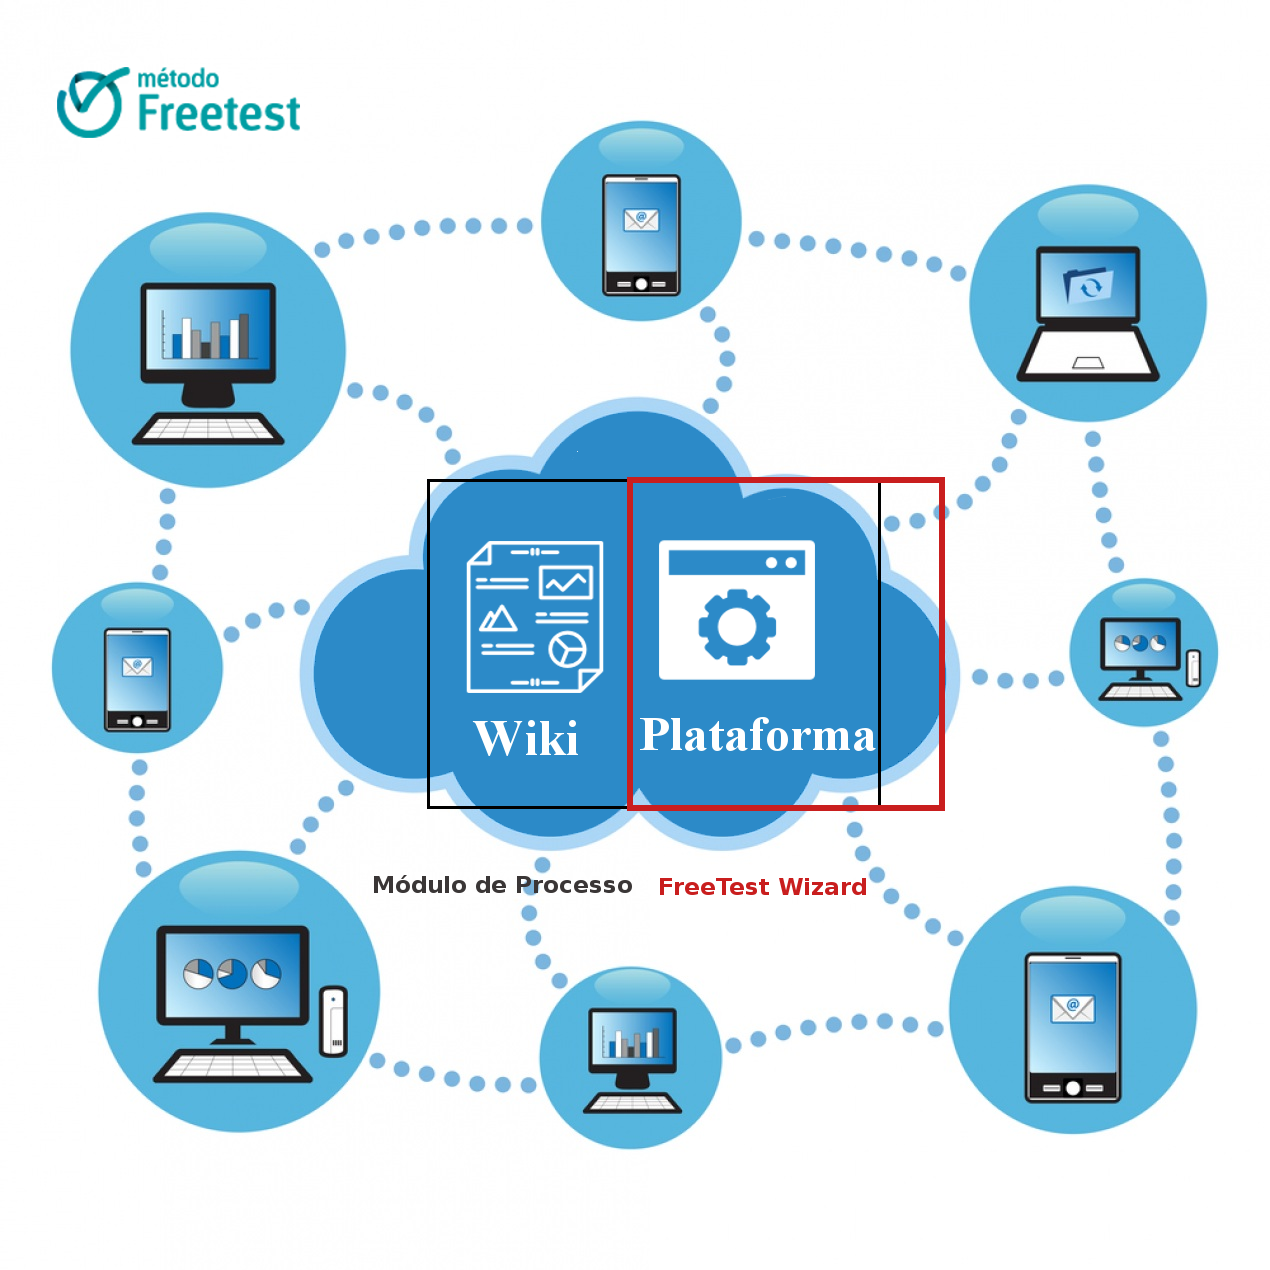
\includegraphics[width=.75\textwidth]{fig/figura63.png}
\caption{Módulos do Sistema: Módulo de processos e Módulo de implantação.}
\label{fig:fig63}
\end{figure}

\subsection{Módulo de Processo}
\label{sec:ferramentaprocesso}

O Módulo do Processo é dividido em duas partes, sendo a primeira uma \textit{wiki}\footnote{http://wiki.freetestframework.com} que contempla toda a parte informativa do processo (vide seção \ref{sec:wikiprocesso}) e a segunda, uma área do software \footnote{http://freetestframework.com} (vide seção \ref{sec:gestordeprocessos}) que abrange toda a manutenção das Áreas de Processo, Práticas Especificas e uma funcionalidade para modelagem de todos os processos da Organização. 

\subsubsection{Construção da \textit{Wiki} para o Processo}
\label{sec:wikiprocesso}

Uma ferramenta tipo \textit{wiki} foi escolhida pois é mais fácil para manter o processo de teste organizado e para se usar esse tipo de ferramenta como gestora de conhecimento. A velocidade em que processos das MPEs precisam se adaptar aos novos cenários do mercado é bem grande. Uma solução eficiente é a \textit{wiki}, que pode prover informações para novos colaboradores e manter os processos atualizados e acessíveis. 

Alguns benefícios de se utilizar uma \textit{wiki} como ferramenta para manutenção do processo podem ser vistos a seguir:

\begin{itemize}
	\item Os processos de teste ficam armazenados numa central de conhecimento;
    \item Novos colaboradores tem um local fácil para aprendizado;
    \item Mudanças são facilmente inseridas;
    \item Aumentamos a eficiência no tempo de aprendizado dos colaboradores;
    \item Ferramenta amplamente conhecida, facilitando a absorção de conhecimento.
\end{itemize}

A \textit{wiki} do processo matem todo o processo FreeTest 2.0, tela de boas vindas, parte informativa do guia de implantação e lista de ferramentas sugeridas para auxilio da execução de cada prática especifica do processo. Se tratando do processo, a estrutura é organizada em Áreas de Processos (AP) e suas respectivas Práticas Especificas (PE) (conforme apresentado na seção \ref{sec:novoprocesso}). No interior de cada PE contém a sua descrição detalhada, dependências, resultados gerados para aquela prática e por fim uma seção que é destinada à parte didática e prática de como implantar (visto na seção \ref{sec:estruturaguiaimplantacao}) a determinada Prática Especifica. A estrutura para cada Prática Especifica (PE) pode ser vista na figura \ref{fig:fig64}.

\begin{figure}[H]
\centering
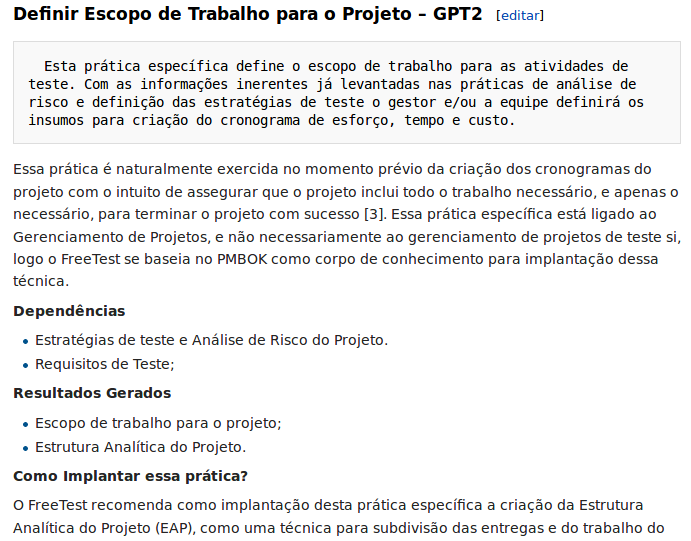
\includegraphics[width=.90\textwidth]{fig/figura64.png}
\caption{Estrutura de uma Prática Especifica do processo.}
\label{fig:fig64}
\end{figure}

Para a criação da wiki do processo do Método FreeTest 2.0 foram utilizados o software Wikimedia \footnote{https://commons.wikimedia.org}, que é distribuído sob licença \textit{Creative Commons} e \textit{open-source} e banco de dados MySQL Server \footnote{https://dev.mysql.com/downloads/mysql/}.

\subsubsection{Construção do Gestor do Processos} 
\label{sec:gestordeprocessos}

Como mencionado o gestor de processos integra uma das partes do módulo de processo. Com a finalidade de criar um ambiente onde as Organizações pudessem manter todos os seus processos, e não somente o processo de teste a ferramenta permite que sejam criados quantas modelagens de processo forem necessários. A modelagem dos processos é feita em BPMN \footnote{http://www.bpmn.org/} (\textit{Business Process Model and Notation}) utilizando o \textit{framework} BPMN.io que foi incorporado à plataforma e que já mencionado na seção \ref{sec:aspectosoperacionais}. A seguir na figura \ref{fig:fig65} é mostrado a interface da ferramenta de modelagem.

\begin{figure}[H]
\centering
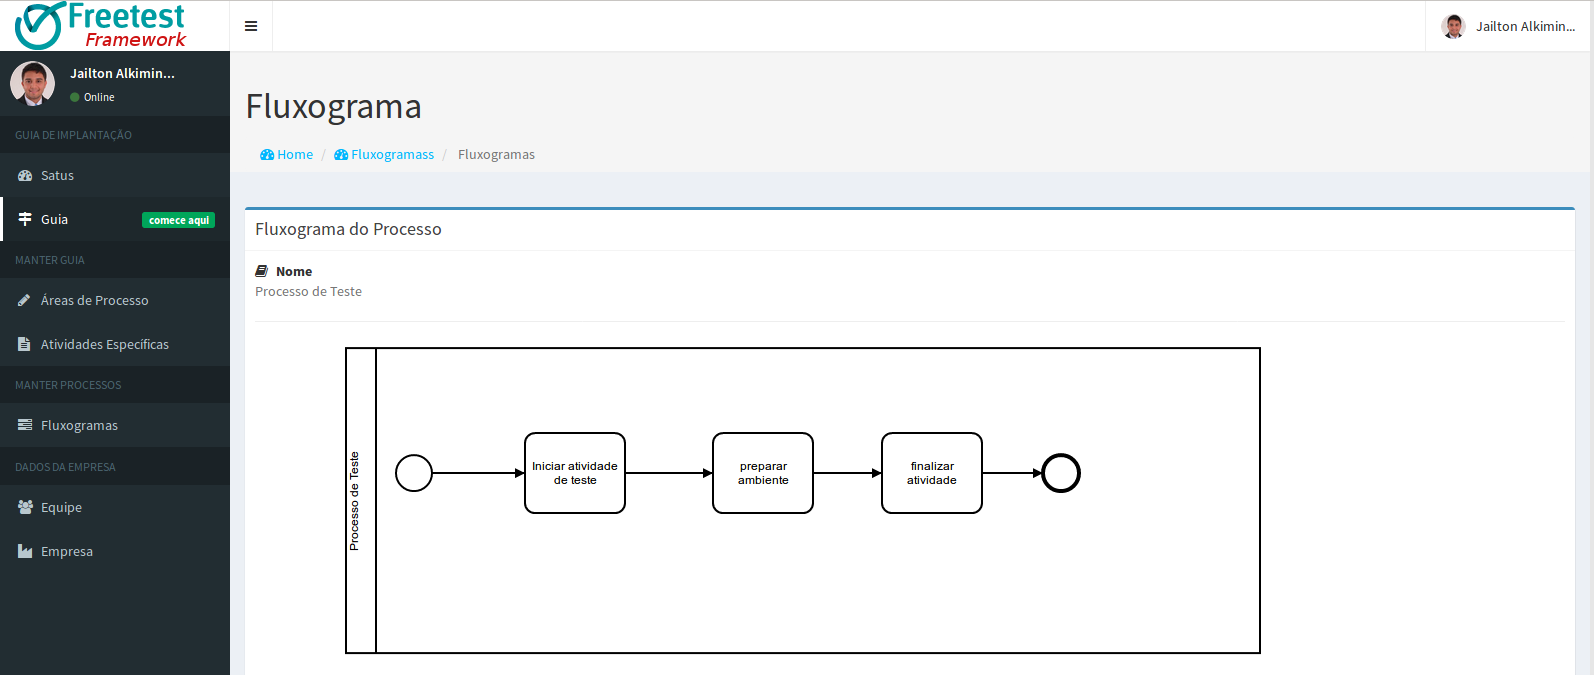
\includegraphics[width=.90\textwidth]{fig/figura65.png}
\caption{Área para modelagem dos processo.}
\label{fig:fig65}
\end{figure}

Como um dos entregáveis deste trabalho foi feita uma modelagem de processo de teste padrão. A modelagem deste processo padrão foi elaborada dentro do contexto do novo processo (seção \ref{sec:novoprocesso}) e entregue como um "modelo de processo de teste" para as Organizações que desejam começar com o nível de maturidade inicial, podendo evoluí-lo conforme suas necessidades. Desta maneira toda Organização recém cadastrada poderá decidir em usar o processo de teste padrão ou criar o seu a partir do zero. A modelagem do processo básico entregue como padrão na ferramenta pode ser vista na figura \ref{fig:fig66}.

\begin{figure}[H]
\centering
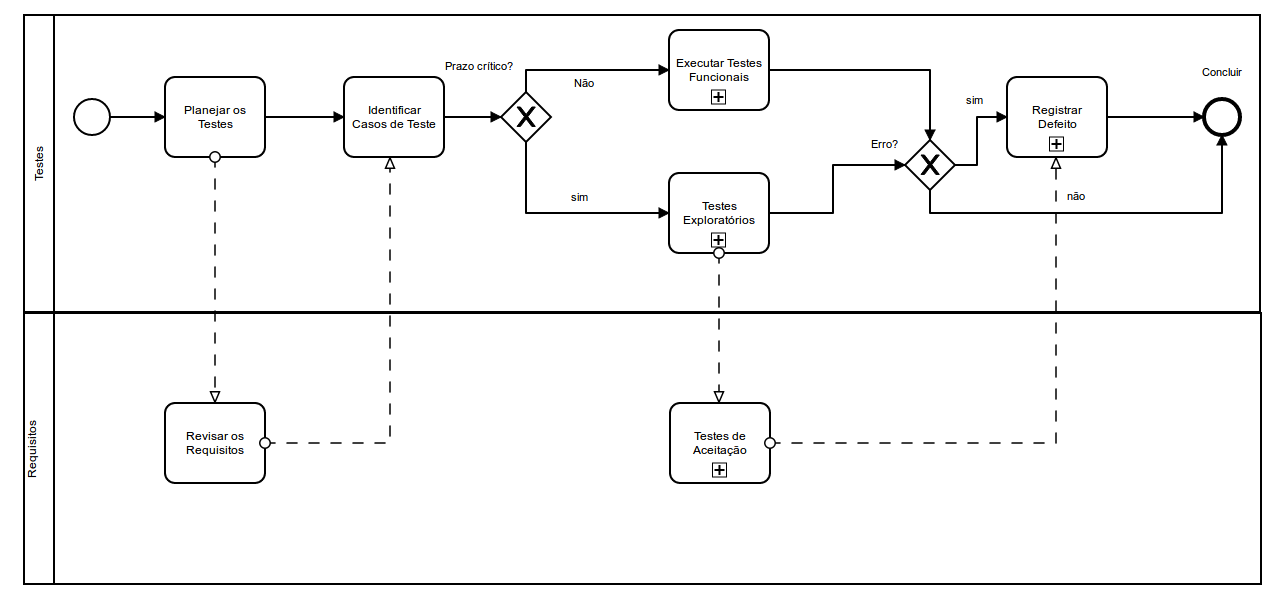
\includegraphics[width=.90\textwidth]{fig/figura66.png}
\caption{Modelagem do processo de teste básico entregue junto com a ferramenta.}
\label{fig:fig66}
\end{figure}

\subsection{Módulo de Implantação}
\label{sec:oguiadeimplantacao}

Como proposta principal deste trabalho, foi criado um módulo do sistema \footnote{http://guide.freetestframework.com} que servirá como o guia de implantação do processo. O guia de implantação é entregue na mesma plataforma do web e no formato \textit{As-a-Service} de forma gratuita. Essa ferramenta representa um grande diferencial desta pesquisa, pois através dela será possível que mesmo MPEs com poucos recursos na área de qualidade de software, possam facilmente implantar, monitorar e definir os marcos para a implantação de seus processos de teste, além de contar com o apoio do guia. O funcionamento geral do Guia de Implantação pode ser visto no Caso de Uso da figura \ref{fig:fig67}. Para maior facilidade na implantação do processo do Método FreeTest 2.0 o Guia de Implantação vem com com informações das Áreas de Processo e Práticas Especificas já populadas, desta maneira auxiliando empresas que não possuem nenhum nível de maturidade em teste à implantar o FreeTest até um nível básico inicial.

\begin{figure}[H]
\centering
\includegraphics[width=.90\textwidth]{fig/figura67.png}
\caption{Modelagem do Caso de Uso representativo do Guia de Implantação.}
\label{fig:fig67}
\end{figure}

O guia de implantação também é dividido em duas partes. Uma parte refere-se ao \textit{"status"} da implantação do processo na Organização e a outra corresponde aos passos necessários para se alcançar um objetivo na implantação de uma prática especifica.

\subsubsection{\textit{Status} Geral de Implantação}
\label{sec:statusimplantacao}

O \textit{status} geral da implantação do processo tem como finalidade exibir indicadores do percentual de que cada área de processo foi implantada. Os indicadores de cada Área de Processo contabilizam quantas práticas especificas foram implantadas e exibem um gráfico tipo "barra" com o percentual de implantação respectivo.

O progresso de cada Área de Processo tem como finalidade dar uma visão geral para a equipe da Organização de como está a implantação do processo. Desta maneira, aumenta o engajamento da equipe e facilita na obtenção de indicadores para metas e planejamento. A figura \ref{fig:fig68} exibe a tela que contempla o \textit{status} geral de implantação.

\begin{figure}[H]
\centering
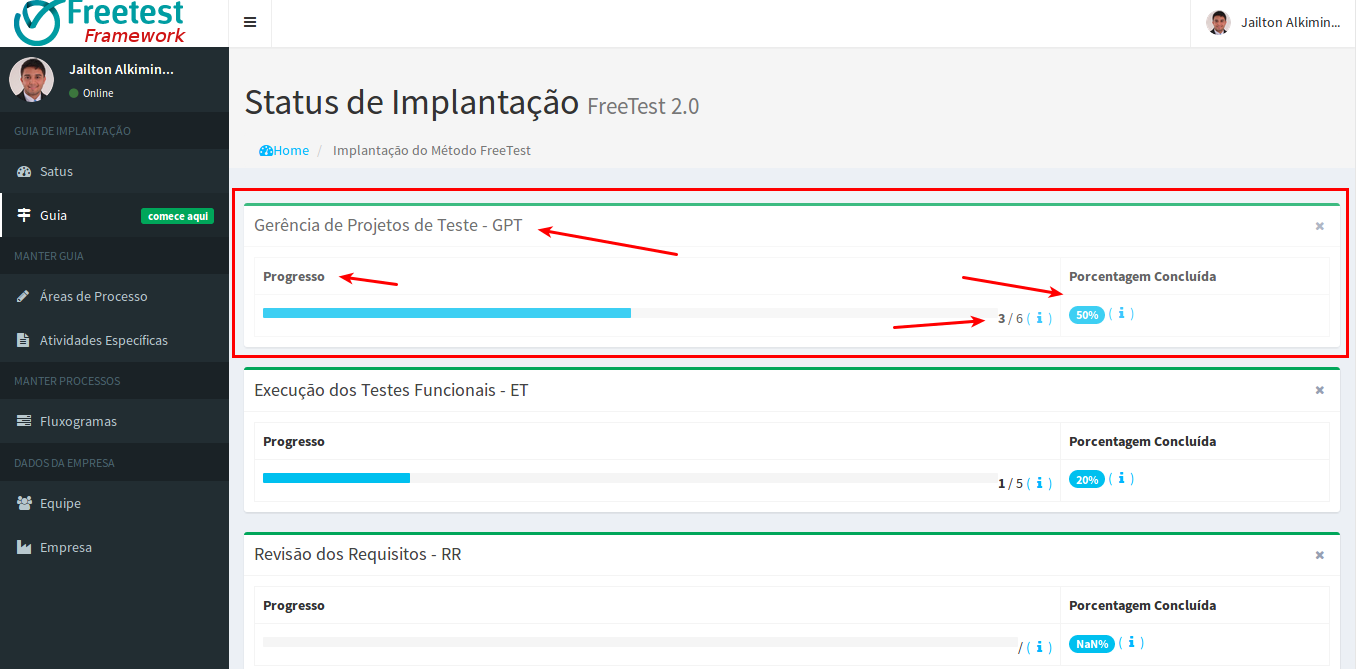
\includegraphics[width=.90\textwidth]{fig/figura68.png}
\caption{Status geral da implantação do processo.}
\label{fig:fig68}
\end{figure}

\subsubsection{Guia de implantação}
\label{sec:passoapassoguia}

O passo-a-passo do guia de implantação auxiliará a Organização a realizar as tarefas/sugestões disponibilizadas na seção \ref{sec:estruturaguiaimplantacao} para alcançar o nível de maturidade desejado, área de processo que deseja implantar e/ou somente determinada Prática Especifica. O guia de implantação é totalmente customizável, o que permite que as Organizações possam futuramente estender o processo do Método FreeTest 2.0 e ajustá-lo, desta forma inserindo novas Áreas de Processo e Práticas Especificas adequadas às necessidades da Organização.

Como mencionado, é possível atualizar e customizar o Guia de Implantação. Neste sentido duas funcionalidades do Guia de Implantação foram criadas para a manutenção e customização das Áreas de Processo e suas respectivas Práticas Especificas, através delas é possível facilmente realizar ajustes necessários e adequações ao processo da Organização. As Figuras \ref{fig:fig69} e \ref{fig:fig610} mostram respectivamente as telas para criação de Áreas de Processos e suas Práticas Especificas.

\begin{figure}[H]
\centering
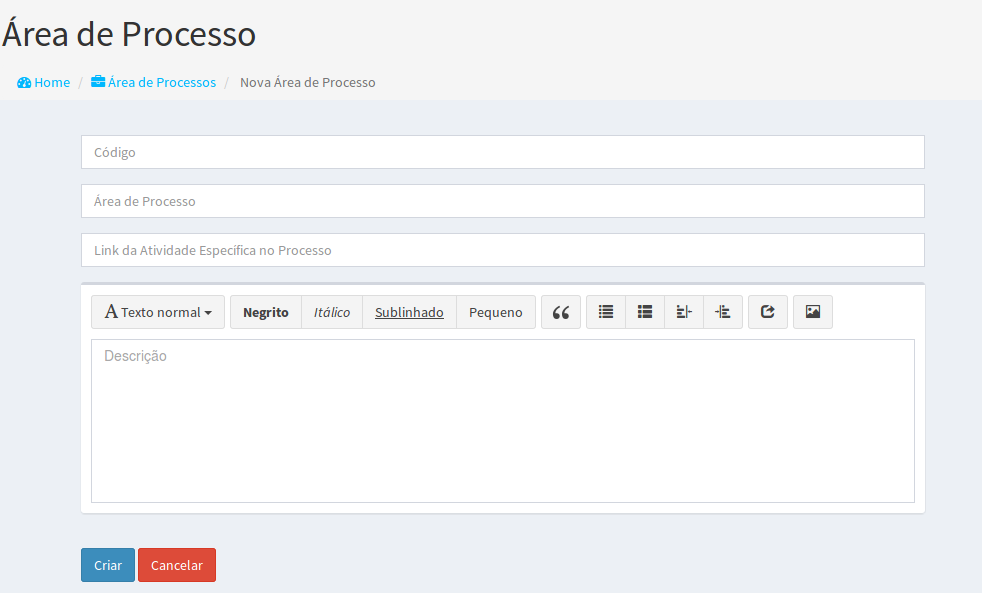
\includegraphics[width=.90\textwidth]{fig/figura69.png}
\caption{Funcionalidade para a criação/manutenção de uma Área de Processo.}
\label{fig:fig69}
\end{figure}

Perceba que na figura \ref{fig:fig69} que mostra a tela de criação de uma Área de Processo requer que o usuário da aplicação informe o código, titulo, link e descrição objetiva da Área de Processo. O link para a Área de Processo será o link da AP na \textit{wiki} do Freetest (mostrado na subseção \ref{sec:wikiprocesso}).

\begin{figure}[H]
\centering
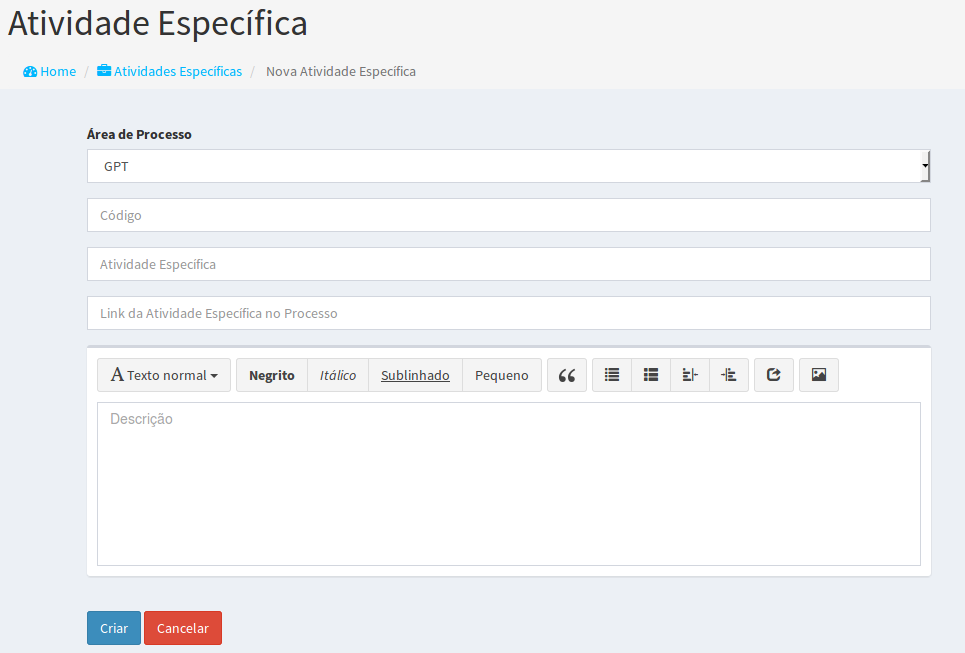
\includegraphics[width=.90\textwidth]{fig/figura610.png}
\caption{Tela para criação/manutenção das Práticas Especificas.}
\label{fig:fig610}
\end{figure}

Seguindo o mesmo padrão da tela de criação da Área de Processo visto na figura \ref{fig:fig68}, a tela para criação de uma Prática Especifica requer que sejam informadas: Área de Processo no qual a prática especifica é vinculada, código da prática, título, link para a prática especifica (direcionado para a \textit{wiki}) e a descrição objetiva.

O Guia de Implantação é apresentado na figura \ref{fig:fig611}. O guia nada mais é que um \textit{wizard} \footnote{http://www.eclipse.org/articles/Article-UI-Guidelines/Contents.html\#Wizards} que auxilia os usuários na implantação das práticas especificas do processo do Método Freetest 2.0 ou até mesmo de práticas especificas criadas pela Organização. Assim que uma nova Área de Processo e suas Práticas Especificas são cadastradas, automaticamente elas são lançadas no Guia de Implantação, desta forma podendo ser executadas pela equipe responsável na implantação do processo, para então, os indicadores de implantação serem atualizados no \textit{Status} Geral de Implantação do Processo.

\begin{figure}[H]
\centering
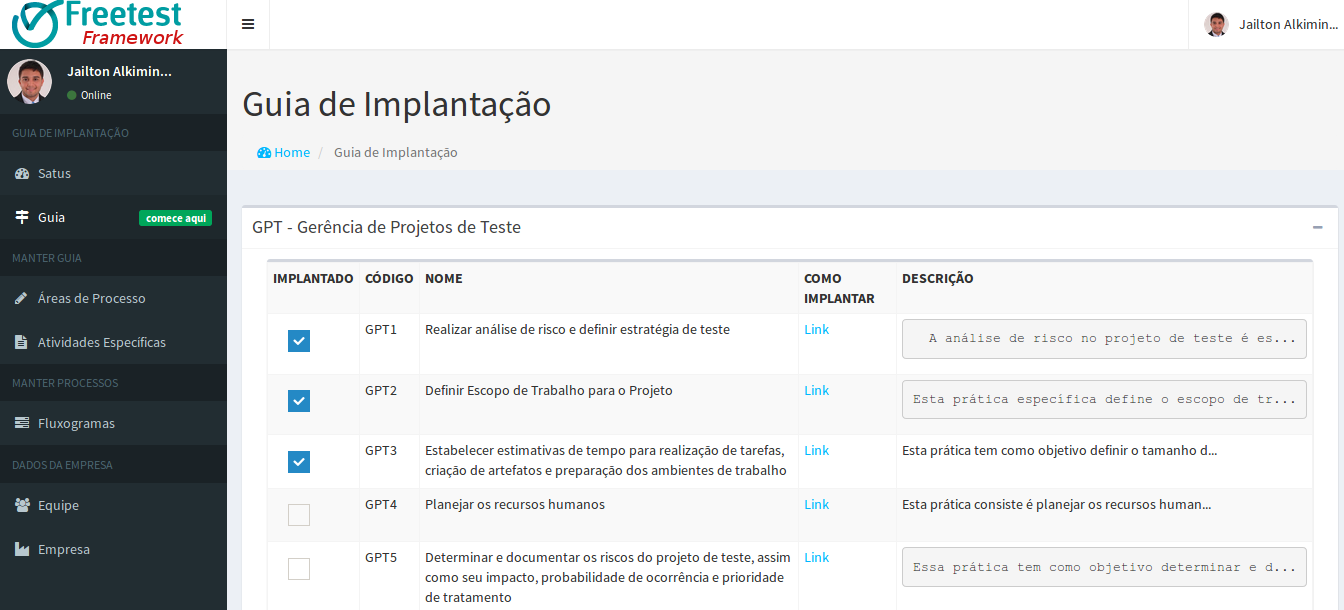
\includegraphics[width=.90\textwidth]{fig/figura611.png}
\caption{Guia de implantação.}
\label{fig:fig611}
\end{figure}


\section{Considerações Finais}
\label{sec:consideracoesfinaiscap6}

Com base no conhecimento empírico dos autores e de revisões da literatura do estado da prática de processos de teste em organizações, principalmente MPEs observou-se que um dos grandes fatores de desistência na implantação de processos de teste é o custo de implantação e o \textit{know-how} técnico necessário para a implantação deste tipo de processo. A partir dessa premissa este trabalho, por meio deste capítulo propôs à criação de ferramentas que apoiassem as Organizações, não somente com um processo de teste, mas também com a sua implantação, manutenção e evolução do mesmo. 

Por fim, através da plataforma web que abrange o Guia de Implantação e o Gestor de processos em conjunto com a \textit{wiki} MPEs poderão de forma fácil, sob demanda e através da web gerenciar seus processos e com auxilio de um \textit{wizard} implantar o processo FreeTest 2.0 intuitivamente. 

\chapter{Conclusão e Trabalhos Futuros}
\label{sec:conclusaoetrabalhosfuturos}

Este capítulo finaliza o estudo, apresentando a conclusão deste e os trabalhos futuros. Este capítulo está organizado da seguinte forma: a seção \ref{sec:finalconclusao} apresenta a conclusão do trabalho e a seção \ref{sec:trabalhosfuturos} apresenta os trabalhos futuros. 

\section{Conclusão}
\label{sec:finalconclusao}

Ao longo dos estudos realizados e do conhecimento empírico dos autores deste trabalho, principalmente com o enfoque em MPEs observou-se que as Organizações devido às suas restrições, principalmente financeira e de recursos humanos, desistem ou deixam em segundo plano uma política de qualidade de software na empresa. Tratando-se de um processo de testes, constatou-se que as limitações de recursos humanos com \textit{know-how} teórico e prático em processos de qualidade, conhecimento de em ferramentas de apoio e informação de como implantar uma dada atividades é um grande limitador, logo com a intenção de apoiar essa situação este trabalho propôs, a melhoria do processo de teste do Método FreeTest, criação de uma ferramenta para manutenção do processo escrito e modelado e um guia de implantação customizável que funciona como um \textit{wizard} de implantação do processo; todo o aparato ferramental e de conhecimento foi distribuído de forma gratuita e num formato \textit{SaaS}.

As melhorias propostas para o processo do Freetest serão de grande contribuição para a melhoria da maturidade das MPEss. A forma que a estrutura do processo foi definida, ou seja, espelhado em modelos de processos já conhecidos internacionalmente, contudo com um embasamento em metodologias ágeis, DevOps e outras boas práticas irão tornar os processos das organizações mais ágeis e com uma visão de automação de algumas tarefas de forma mais fácil e barata, pois a automação quando bem planejada e executada contribui na redução dos custos. 

Com o intuito de apoiar às organizações, foram desenvolvidos ferramentas de apoio à manutenção dos processos da empresa, entregue a comunidade no formato web, podendo ser acessado por qualquer um que tenha um cadastro na mesma. Além de possibilitar o acesso aos processos da organização é possível evoluir ou estender o processo do Método FreeTest, o que torna uma ferramenta flexível e aderente à organização. 

Por fim, com a ajuda do guia de implantação será possível que organizações, principalmente com o perfil de micro e pequenas empresas possam implantar o processo de teste de forma autônoma e prática com o apoio do \textit{wizard} de implantação, desta maneira, reduzindo custos com consultorias técnicas e com ferramentas de apoio pagas, já que o método proposto aconselha o uso de ferramentas de código aberto.

\section{Trabalhos Futuros}
\label{sec:trabalhosfuturos}

Esse trabalho abre um precedente no que diz respeito a entrega de um processo de teste de software como serviço. A cerca dos estudos realizados sobre automação estima-se que em outra fase será possível tornar tarefas automatizadas a partir do processo modelado na plataforma web, desta maneira podendo monitorar ou até mesmo executar determinadas tarefas via ambiente totalmente virtualizado. 

Acerca dos estudos realizados sobre DevOps, acredita-se que a criação e manutenção de ambientes de teste poderá ser mantida dentro da plataforma, transformando a infraestrutura como código (\textit{infraestructure as a code}) e utilizando a virtualização de ambientes de teste de maneira automáticas e de fácil acesso através da plataforma web. Será possível então reduzir custos com ambientes de trabalho e reduzir típicos falsos erros oriundos de ambientes, corroborando então com práticas de Entrega Contínua (\textit{Continuous Delivery}). 

Outra proposta de trabalho futuro é a incorporação de um Modelo de Competências relacionados ao teste de software. Buscando na literatura não foi encontrado nenhum processo de uso específico que utilize um Modelo de Competência para auxiliar as organizações a determinar com base nas competências o melhor papel para determinada área de atuação. Desta maneira como trabalhos futuros esperamos evoluir o método FreeTest com um Modelo de Competência baseado no SWECOM (\textit{Software Engineering Capability Model}) \cite{swecom2017} focado em micro e pequenas empresas. 
%\input{./tex/cap_VII}

%------------------------------------------------------------ BIBLIOGRAFIA %
\cleardoublepage
\nocite{*} %%% Retire esta linha para gerar a bibliografia com apenas as
           %%% referências usadas no seu texto!
\arial
\bibliography{./bib/modelo-tese} %%% Nomes dos seus arquivos .bib
\label{ref-bib}

%--------------------------------------------------------------- APÊDICES %
\apendices

\chapter{\textit{Case} de execução do FreeTest 2.0}
\label{sec:caseexecucaofreetest20}


\section{Case: MPE-PDV - Fictício}
\label{sec:apendicempe}

\subsection{A instituição}

Fundada em 1998 por seu proprietário João da Silva a MPE-PDV Sistemas hoje está consolidada como uma empresa líder no mercado de software para PDV (Ponto de Venda). Com sede em Goiânia - GO atende todo o Brasil com sua solução web voltada para Pontos de Venda, através do seu carro chefe o MPE-PDV, que obviamente leva o mesmo nome da empresa. Empresa com vinte funcionários, divididos dentro outros departamentos por suporte e desenvolvimento, que ocupam o maior quadro de pessoas da organização.

\subsection{O desafio}

A MPE-PDV é uma empresa como várias outras, possui um software carro chefe que é vendido sob um modelo de negócio do tipo “contrato de prestação de serviços”, no qual a fornecedora (MPE-PDV) “aluga” o software para seu cliente (consumidor), que por sua vez, paga um valor mensal que é determinado pelo o uso do software e pela quantidade de usuários que seu cliente possui para utilizar o sistema.

Por ser uma empresa comprometida em atender todos os seus mais de 150 clientes em todo o Brasil, a MPE-PDV de dois em dois meses gera novas versões do seu software, com o intuito de levar melhorias aos seus clientes e correções de \textit{bugs}, quando encontrados. Isso é importante, pois sempre que há uma mudança na lei que impacta seu software ou um de seus clientes solicita uma melhoria a MPE-PDV deve em tempo hábil desenvolvê-la, testá-la (ou não) sempre que possível.

Sua equipe de desenvolvimento e teste trabalha sempre a todo o vapor, em outras palavras, sempre apagando incêndios! A equipe de testes é composta por dois analistas, que realizam testes funcionais na aplicação e relatam os erros encontrados no próprio sistema de \textit{help desk}. O sistema de \textit{Help Desk} é onde todos as demandas, tanto de melhorias (externas ou internas), quanto correções são registradas. A quantidade de erros encontradas é relativamente grande, mas poderia ser maior... Uma das justificativas da equipe de testes é que além da \textit{“demora de se criar os ambientes ideais para se testar a aplicação, vira e mexe um build vem instável”}. Isso quer dizer, que a aplicação não executa corretamente, em outras palavras, é um grande transtorno, pois como a equipe de testes não tem acesso ou apoia a criação dos \textit{builds} não consegue detectar este tipo de problema de forma precoce, deste modo dependendo da ajuda de um desenvolvedor (que provavelmente está ocupado).

Outro grande problema relatado pela equipe de testes é que alguns erros triviais são encontrados, no entanto a questão é que muitos destes erros são impeditivos, isso quer dizer que é impossível testar novos cenários até a correção deste erro. Senão bastassem os desafios diários, o MPE-PDV é um software legado, com baixo nível de documentação, com inúmeras regras de negócio complexas e interdependentes e com uma arquitetura monolítica, que segundo os testadores dificultam ainda mais o seu trabalho.

Este cenário é cíclico e se repete a cada projeto para lançar uma nova versão. Como as demandas nunca param de chegar e os prazos são sempre curtos, muitas vezes é necessário realizar entregas do MPE-PDV sem a quantidade de testes necessárias, mas qual é a quantidade de testes necessária? Aí já é outra história...

\subsection{A solução}

Após a implantação do Método FreeTest 2.0 a MPE-PDV Sistemas obteve algumas melhorias. Por escolha da MPE-PDV o Freetest 2.0 foi implantado até o nível 4 de maturidade, a decisão foi feita pela equipe técnica envolvida na implantação do processo, o motivo foi que, segundo a equipe boa parte dos gargalos que ela enfrentavam poderiam ser resolvidos com as práticas especificas disponíveis no nível quatro de maturidade.

Agora graças as práticas de gerenciamento de projetos de teste (área de processo GPT) a equipe de testes está mais ativa no planejamento das atividades, pois consegue realizar análises de risco, definir estratégias, escopos do que testar e criar estimativas mais fieis ao que será executado, pois agora os próprios testadores estão aplicando seu \textit{know-how} para definir o planejamento de suas atividades. O mais importante é que, com essas práticas de gerenciamento do projeto de testes, a equipe de testes se tornou mais ativa nos projetos, conseguindo interagir desde concepção, isso tornou a equipe mais engajada, melhorou o trabalho em equipe e reduziu ruídos na comunicação.

Com as atividades planejadas, cronogramas bem definidos e todos sabendo o que devem fazer agora ficou mais fácil executar os testes funcionais, isso porque após adotar o FreeTest 2.0, novas ferramentas de apoio foram implantadas para ajudar a equipe de testes, entre elas o TestLink e MantisBT (área de processo ET). O Testlink ajuda na especificação e execução dos casos de teste e torna o trabalho em equipe mais dinâmico e transparente, pois qualquer um da organização consegue acompanhar as atividades de teste. O MantisBT, por outro lado, permite que os erros sejam reportados da forma devida, desta forma não sendo mais necessário usar a antiga ferramenta de Help Desk para reportar erros e melhorias, pois agora ela será somente de uso do suporte e dos clientes. Com uma ferramenta adequada para reportar os erros, identificação, especificação e execução dos casos de teste ficou mais fácil gerar dados que serão utilizados como métricas ao fim dos projetos, isso contribuirá para a melhoria contínua do processo na empresa.

Outro problema que era corriqueiro na MPE-PDV Sistemas era a grande quantidade de \textit{builds} falhas e erros inseridos. No entanto, com a ajuda de novas abordagens sugeridas pelo FreeTest 2.0 este número de problemas foi reduzido, pois agora a equipe de desenvolvimento com auxilio de ferramentas de gerência de configuração (área de processo GCT) e análise estática de código, tem feito a revisão de código fonte e aplicado \textit{style checkers} e \textit{bugs checkers} (área de processo AES), desta maneira, com a colaboração da equipe de desenvolvimento erros tem sido encontrados prematuramente. Um ganho que vale ressaltar foi com a aplicação de testes de regressão (área de processo TRG), pois pela própria natureza do software com uma grande quantidade de regras de negócios interdependentes, era normal que uma alteração pontual em uma região do software impactasse outra, contudo agora com a aplicação de testes de regressão e apoio das ferramentas de teste e futuramente automação dos casos de teste ficou mais fácil evidenciar estes \textit{bugs}. Estas práticas surtiram grande resultados na empresa e animou a equipe de suporte que esporadicamente ouvia de seus usuários reclamações como, “A funcionalidade XPTO que funcionava na versão anterior, não funciona mais!”.

Foi natural que com a implantação de ferramentas de gestão e controle dos testes, dados de execução, \textit{bugs} registrados e quantidade de re-testes feitos, tais dados se tornassem insumos para métricas (área de processo MED). Com isso a empresa pode coletar e analisar os dados e utilizá-los para melhoria contínua do processo, produto e até mesmo no planejamento estratégico da empresa! Com informações mais fidedignas, artefatos e um conjunto de ferramentas de apoio a empresa logo começou a automatizar vários funcionalidades do MPE-PDV, desta maneira, criando constantemente \textit{scripts} de teste para regressão (área de processo TRG) e testes de aceitação (área de processo TDA) que são executados dentro de uma ambiente totalmente integrado, graças a uma ferramenta de integração contínua (área de processo INC), também proposta pelo FreeTest 2.0, de agora em diante, não só os testes escritos pelos testadores são executados pela integração contínua, como também toda a geração de \textit{build} e \textit{deploy} é feita de forma automática, aumentando o feedback, evitando perca de tempo com criação do ambiente de testes e gerando rápidas respostas para corrigir eventuais falhas.

Agora com as práticas de teste bem definidas, métricas de todos os projetos e com o apoio de diversas ferramentas a empresa MPE-PDV já pensa em expandir sua operação e criar uma nova ferramenta no mesmo seguimento, contudo com um modelo de negócio \textit{As-a-Service} e para isso já estuda como irá desenvolver, testar e entregar seu software de forma contínua (área de processo TCA).
%\chapter{Termo de Consentimento Livre e Esclarecido}
Você está sendo convidado(a) para participar, como voluntário(a), de uma pesquisa. Meu nome é \textbf{Tiago do Carmo Nogueira}, sou aluno do Programa de Mestrado em Ciência da Computação da Universidade Federal de Goiás.

A presente pesquisa está sendo realizada como parte de uma dissertação de mestrado em Ciência da Computação. Tem como objetivo investigar as dificuldades e similaridades na Experiência de Usuários cegos e videntes (que enxergam) nas novas tendências na Web.

Em caso de dúvida sobre a pesquisa, você poderá entrar em contato com o pesquisador responsável, \textbf{Tiago do Carmo Nogueira} por e-mail: tiago.nogueira@bag.ifmt.edu.br. Em casos de dúvidas sobre os seus direitos como participante nesta pesquisa, você poderá entrar em contato com o \textbf{Comitê de Ética em Pesquisa da Universidade Federal de Goiás}, nos telefones: \textbf{3521-1075} ou \textbf{3521-1076}.

\begin{center}
\textbf{CONSENTIMENTO DA PARTICIPAÇÃO DA PESSOA COMO SUJEITO DA PESQUISA}
\end{center}

Eu entendo que as informações e gravações são apenas para fins de investigação e que o meu nome e imagem não vai ser usado para qualquer outra finalidade. Eu renuncio quaisquer direitos sobre as gravações e entendo que as gravações podem ser copiadas e usadas apenas para esta pesquisa. 

Eu compreendo que a participação neste estudo é voluntária e eu concordo em levantar imediatamente quaisquer preocupações ou desconforto durante as tarefas proposta pela pesquisa com o(s) pesquisador responsável.

Por favor, assine abaixo para indicar que você leu e entendeu as informações neste formulário e que quaisquer dúvidas que possa ter sobre a sessão foram respondidas.

\begin{center}
\begin{tabular}{p{7.2cm}}
\hline
\multicolumn{1}{c}{Participante da Pesquisa}\\
\end{tabular}
\end{center}
%\chapter{Questionário de Identificação dos Sujeitos de Pesquisa}
\begin{center}
\begin{longtable}{l}
\multicolumn{1}{c}{
Cegueira Total (congênita)(  )         Cegueira Total (adquirida)(  )          Usuário (vidente)(  )
}\\ 
\hline
\multicolumn{1}{c}{} \\ 
\multicolumn{1}{c}{\textbf{Informações Pessoais}} \\ 
01. Nome completo? \\ 
\hline
\multicolumn{1}{|l|}{} \\ 
\hline
02. Data de nascimento? \\ 
\hline
\multicolumn{1}{|l|}{} \\ 
\hline
03. Qual seu sexo? \\ 
\hline
\multicolumn{1}{|l|}{} \\ 
\hline
\multicolumn{1}{c}{\textbf{Informações Educacionais}} \\ 
04. Qual seu grau de instrução? Em que ano terminou? \\ 
\hline
\multicolumn{1}{|l|}{} \\ 
\hline
05. Se 3º grau, qual nome do curso? Quando ingressou? \\ 
\hline
\multicolumn{1}{|l|}{} \\ 
\hline
\multicolumn{1}{c}{\textbf{Experiência Profissional}} \\ 
06. Qual sua profissão? \\ 
\hline
\multicolumn{1}{|l|}{} \\ 
\hline
07. Há quanto tempo se encontra nessa profissão? \\ 
(   ) Menos de 1 ano. \\ 
(   ) Entre 1 ano a 2 anos. \\ 
(   ) Entre 2 anos a 4 anos. \\ 
(   ) Mais de 4 anos. \\ 
\multicolumn{1}{c}{\textbf{Experiência Computacional}} \\ 
08. Há quanto tempo você utiliza computador? \\ 
(   ) Menos de 1 ano. \\ 
(   ) Entre 1 ano a 2 anos. \\ 
(   ) Entre 2 anos a 4 anos. \\ 
(   ) Mais de 4 anos. \\ 
09. Em que local você utiliza computador? (Pode marcar mais de uma opção). \\ 
(   ) Casa. \\ 
(   ) Trabalho \\ 
(   ) Escola. \\ 
(   ) Outros? \\ 
10. Em média, quantas horas por semana você utiliza o computador? \\ 
(   ) Menos de 2 horas. \\ 
(   ) Entre 2 a 5 horas \\ 
(   ) Entre 5 a 10 horas. \\ 
(   ) Mais de 10 horas. \\ 
11. Já envolveu em algum projeto de usabilidade/acessibilidade? \\ 
(   ) Sim.\\     (   ) Não. \\ 
12. Já participou de algum teste de usabilidade? Se sim, qual tipo de site você acessou? \\ 
\hline
\multicolumn{1}{|l|}{} \\ 
\hline
13. Qual ferramenta assistiva tem costume de usar? \\ 
\hline
\multicolumn{1}{|l|}{} \\ 
\hline
\end{longtable}
\end{center}
%\chapter{Questionário Affect Grid (UX)}
\label{sec:questionarioaffectgrid}
%Identificação da categoria do teste
\begin{tabular}{lllllll}
\hline
\multicolumn{7}{|c|}{\textbf{Identificação da Avaliação}} \\ 
\hline
\multicolumn{1}{|l|}{\textbf{Aplicação:}} & \multicolumn{1}{l|}{(   ) S01} & \multicolumn{1}{l|}{(   ) S02} & \multicolumn{1}{l|}{(   ) S03} & \multicolumn{1}{l|}{(   ) S04} & \multicolumn{1}{l|}{(   ) S05} & \multicolumn{1}{l|}{(   ) S06} \\ 
\hline
\end{tabular}

\begin{table}[ht]
\centering
\begin{longtable}{llllllllll}
\multicolumn{10}{l}{\textbf{Tarefa 01}} \\ 
\multicolumn{10}{c}{Marque com um \textbf{X} em uma escala de 1 a 9 como você se sentiu ao realizar esta tarefa?} \\ 
\cline{2-10}
\multicolumn{1}{l|}{} & \multicolumn{1}{c|}{1} & \multicolumn{1}{c|}{2} & \multicolumn{1}{c|}{3} & \multicolumn{1}{c|}{4} & \multicolumn{1}{c|}{5} & \multicolumn{1}{c|}{6} & \multicolumn{1}{c|}{7} & \multicolumn{1}{c|}{8} & \multicolumn{1}{c|}{9} \\ 
\cline{2-10}
\multicolumn{1}{p{7.2cm}}{Desprazer-Prazer} & \multicolumn{1}{c}{( )} & \multicolumn{1}{c}{( )} & \multicolumn{1}{c}{( )} & \multicolumn{1}{c}{( )} & \multicolumn{1}{c}{( )} & \multicolumn{1}{c}{( )} & \multicolumn{1}{c}{( )} & \multicolumn{1}{c}{( )} & \multicolumn{1}{c}{( )} \\ 
\multicolumn{1}{p{7.2cm}}{Sonolento-Animado} & \multicolumn{1}{c}{( )} & \multicolumn{1}{c}{( )} & \multicolumn{1}{c}{( )} & \multicolumn{1}{c}{( )} & \multicolumn{1}{c}{( )} & \multicolumn{1}{c}{( )} & \multicolumn{1}{c}{( )} & \multicolumn{1}{c}{( )} & \multicolumn{1}{c}{( )} \\ 
\multicolumn{10}{l}{\textbf{Tarefa 02}} \\ 
\multicolumn{10}{c}{Marque com um \textbf{X} em uma escala de 1 a 9 como você se sentiu ao realizar esta tarefa?} \\ 
\cline{2-10}
\multicolumn{1}{l|}{} & \multicolumn{1}{c|}{1} & \multicolumn{1}{c|}{2} & \multicolumn{1}{c|}{3} & \multicolumn{1}{c|}{4} & \multicolumn{1}{c|}{5} & \multicolumn{1}{c|}{6} & \multicolumn{1}{c|}{7} & \multicolumn{1}{c|}{8} & \multicolumn{1}{c|}{9} \\ 
\cline{2-10}
\multicolumn{1}{p{7.2cm}}{Desprazer-Prazer} & \multicolumn{1}{c}{( )} & \multicolumn{1}{c}{( )} & \multicolumn{1}{c}{( )} & \multicolumn{1}{c}{( )} & \multicolumn{1}{c}{( )} & \multicolumn{1}{c}{( )} & \multicolumn{1}{c}{( )} & \multicolumn{1}{c}{( )} & \multicolumn{1}{c}{( )} \\ 
\multicolumn{1}{p{7.2cm}}{Sonolento-Animado} & \multicolumn{1}{c}{( )} & \multicolumn{1}{c}{( )} & \multicolumn{1}{c}{( )} & \multicolumn{1}{c}{( )} & \multicolumn{1}{c}{( )} & \multicolumn{1}{c}{( )} & \multicolumn{1}{c}{( )} & \multicolumn{1}{c}{( )} & \multicolumn{1}{c}{( )} \\ 
\multicolumn{10}{l}{\textbf{Tarefa 03}} \\ 
\multicolumn{10}{c}{Marque com um \textbf{X} em uma escala de 1 a 9 como você se sentiu ao realizar esta tarefa?} \\ 
\cline{2-10}
\multicolumn{1}{l|}{} & \multicolumn{1}{c|}{1} & \multicolumn{1}{c|}{2} & \multicolumn{1}{c|}{3} & \multicolumn{1}{c|}{4} & \multicolumn{1}{c|}{5} & \multicolumn{1}{c|}{6} & \multicolumn{1}{c|}{7} & \multicolumn{1}{c|}{8} & \multicolumn{1}{c|}{9} \\ 
\cline{2-10}
\multicolumn{1}{p{7.2cm}}{Desprazer-Prazer} & \multicolumn{1}{c}{( )} & \multicolumn{1}{c}{( )} & \multicolumn{1}{c}{( )} & \multicolumn{1}{c}{( )} & \multicolumn{1}{c}{( )} & \multicolumn{1}{c}{( )} & \multicolumn{1}{c}{( )} & \multicolumn{1}{c}{( )} & \multicolumn{1}{c}{( )} \\ 
\multicolumn{1}{p{7.2cm}}{Sonolento-Animado} & \multicolumn{1}{c}{( )} & \multicolumn{1}{c}{( )} & \multicolumn{1}{c}{( )} & \multicolumn{1}{c}{( )} & \multicolumn{1}{c}{( )} & \multicolumn{1}{c}{( )} & \multicolumn{1}{c}{( )} & \multicolumn{1}{c}{( )} & \multicolumn{1}{c}{( )} \\ 
\multicolumn{10}{l}{\textbf{Tarefa 04}} \\ 
\multicolumn{10}{c}{Marque com um \textbf{X} em uma escala de 1 a 9 como você se sentiu ao realizar esta tarefa?} \\ 
\cline{2-10}
\multicolumn{1}{l|}{} & \multicolumn{1}{c|}{1} & \multicolumn{1}{c|}{2} & \multicolumn{1}{c|}{3} & \multicolumn{1}{c|}{4} & \multicolumn{1}{c|}{5} & \multicolumn{1}{c|}{6} & \multicolumn{1}{c|}{7} & \multicolumn{1}{c|}{8} & \multicolumn{1}{c|}{9} \\ 
\cline{2-10}
\multicolumn{1}{p{7.2cm}}{Desprazer-Prazer} & \multicolumn{1}{c}{( )} & \multicolumn{1}{c}{( )} & \multicolumn{1}{c}{( )} & \multicolumn{1}{c}{( )} & \multicolumn{1}{c}{( )} & \multicolumn{1}{c}{( )} & \multicolumn{1}{c}{( )} & \multicolumn{1}{c}{( )} & \multicolumn{1}{c}{( )} \\ 
\multicolumn{1}{p{7.2cm}}{Sonolento-Animado} & \multicolumn{1}{c}{( )} & \multicolumn{1}{c}{( )} & \multicolumn{1}{c}{( )} & \multicolumn{1}{c}{( )} & \multicolumn{1}{c}{( )} & \multicolumn{1}{c}{( )} & \multicolumn{1}{c}{( )} & \multicolumn{1}{c}{( )} & \multicolumn{1}{c}{( )} \\ 
\multicolumn{10}{l}{\textbf{Tarefa 05}} \\ 
\multicolumn{10}{c}{Marque com um \textbf{X} em uma escala de 1 a 9 como você se sentiu ao realizar esta tarefa?} \\ 
\cline{2-10}
\multicolumn{1}{l|}{} & \multicolumn{1}{c|}{1} & \multicolumn{1}{c|}{2} & \multicolumn{1}{c|}{3} & \multicolumn{1}{c|}{4} & \multicolumn{1}{c|}{5} & \multicolumn{1}{c|}{6} & \multicolumn{1}{c|}{7} & \multicolumn{1}{c|}{8} & \multicolumn{1}{c|}{9} \\ 
\cline{2-10}
\multicolumn{1}{p{7.2cm}}{Desprazer-Prazer} & \multicolumn{1}{c}{( )} & \multicolumn{1}{c}{( )} & \multicolumn{1}{c}{( )} & \multicolumn{1}{c}{( )} & \multicolumn{1}{c}{( )} & \multicolumn{1}{c}{( )} & \multicolumn{1}{c}{( )} & \multicolumn{1}{c}{( )} & \multicolumn{1}{c}{( )} \\ 
\multicolumn{1}{p{7.2cm}}{Sonolento-Animado} & \multicolumn{1}{c}{( )} & \multicolumn{1}{c}{( )} & \multicolumn{1}{c}{( )} & \multicolumn{1}{c}{( )} & \multicolumn{1}{c}{( )} & \multicolumn{1}{c}{( )} & \multicolumn{1}{c}{( )} & \multicolumn{1}{c}{( )} & \multicolumn{1}{c}{( )} \\
\multicolumn{10}{l}{\textbf{Tarefa 06}} \\ 
\multicolumn{10}{c}{Marque com um \textbf{X} em uma escala de 1 a 9 como você se sentiu ao realizar esta tarefa?} \\ 
\cline{2-10}
\multicolumn{1}{l|}{} & \multicolumn{1}{c|}{1} & \multicolumn{1}{c|}{2} & \multicolumn{1}{c|}{3} & \multicolumn{1}{c|}{4} & \multicolumn{1}{c|}{5} & \multicolumn{1}{c|}{6} & \multicolumn{1}{c|}{7} & \multicolumn{1}{c|}{8} & \multicolumn{1}{c|}{9} \\ 
\cline{2-10}
\multicolumn{1}{p{7.2cm}}{Desprazer-Prazer} & \multicolumn{1}{c}{( )} & \multicolumn{1}{c}{( )} & \multicolumn{1}{c}{( )} & \multicolumn{1}{c}{( )} & \multicolumn{1}{c}{( )} & \multicolumn{1}{c}{( )} & \multicolumn{1}{c}{( )} & \multicolumn{1}{c}{( )} & \multicolumn{1}{c}{( )} \\ 
\multicolumn{1}{p{7.2cm}}{Sonolento-Animado} & \multicolumn{1}{c}{( )} & \multicolumn{1}{c}{( )} & \multicolumn{1}{c}{( )} & \multicolumn{1}{c}{( )} & \multicolumn{1}{c}{( )} & \multicolumn{1}{c}{( )} & \multicolumn{1}{c}{( )} & \multicolumn{1}{c}{( )} & \multicolumn{1}{c}{( )} \\ 
\end{longtable}
\end{table}
%\chapter{Questionário PANAS (UX)}
\label{sec:questionarioapanas}
\begin{tabular}{lllllll}
\hline
\multicolumn{7}{|c|}{\textbf{Identificação da Avaliação}} \\ 
\hline
\multicolumn{1}{|l|}{\textbf{Aplicação:}} & \multicolumn{1}{l|}{(   ) S01} & \multicolumn{1}{l|}{(   ) S02} & \multicolumn{1}{l|}{(   ) S03} & \multicolumn{1}{l|}{(   ) S04} & \multicolumn{1}{l|}{(   ) S05} & \multicolumn{1}{l|}{(   ) S06} \\ 
\hline
\end{tabular}

\begin{table}[ht]
\centering
\begin{longtable}{|p{274pt}|l|l|l|l|l|}
\hline
\parbox{274pt}{
Por favor, marque com um \textbf{X} aquela opção que melhor expressar seus sentimentos no exato momento em que você lê as frases. Seja o mais sincero possível, e lembre-se de que não existe resposta certa ou errada.
}
&\parbox{19pt}{\centering \begin{turn}{90}Muito pouco ou nada\end{turn}}  
&\parbox{19pt}{\centering \begin{turn}{90}Um pouco\end{turn}}  
&\parbox{19pt}{\centering \begin{turn}{90}Moderadamente\end{turn}}  
&\parbox{19pt}{\centering \begin{turn}{90}Muito\end{turn}}  
&\parbox{19pt}{\centering \begin{turn}{90}Excessivamente\end{turn}}  \\ 
\hline
01. Sinto-me interessado(a) & \multicolumn{1}{c|}{(   )} & \multicolumn{1}{c|}{(   )} & \multicolumn{1}{c|}{(   )} & \multicolumn{1}{c|}{(   )} & \multicolumn{1}{c|}{(   )} \\ 
\hline
02. Sinto-me irritado(a) & \multicolumn{1}{c|}{(   )} & \multicolumn{1}{c|}{(   )} & \multicolumn{1}{c|}{(   )} & \multicolumn{1}{c|}{(   )} & \multicolumn{1}{c|}{(   )} \\ 
\hline
03. Sinto-me angustiado(a) & \multicolumn{1}{c|}{(   )} & \multicolumn{1}{c|}{(   )} & \multicolumn{1}{c|}{(   )} & \multicolumn{1}{c|}{(   )} & \multicolumn{1}{c|}{(   )} \\ 
\hline
04. Sinto-me em "estado de alerta" & \multicolumn{1}{c|}{(   )} & \multicolumn{1}{c|}{(   )} & \multicolumn{1}{c|}{(   )} & \multicolumn{1}{c|}{(   )} & \multicolumn{1}{c|}{(   )} \\ 
\hline
05. Sinto-me animado(a) & \multicolumn{1}{c|}{(   )} & \multicolumn{1}{c|}{(   )} & \multicolumn{1}{c|}{(   )} & \multicolumn{1}{c|}{(   )} & \multicolumn{1}{c|}{(   )} \\ 
\hline
06. Sinto-me envergonhado(a) & \multicolumn{1}{c|}{(   )} & \multicolumn{1}{c|}{(   )} & \multicolumn{1}{c|}{(   )} & \multicolumn{1}{c|}{(   )} & \multicolumn{1}{c|}{(   )} \\ 
\hline
07. Sinto-me transtornado(a) & \multicolumn{1}{c|}{(   )} & \multicolumn{1}{c|}{(   )} & \multicolumn{1}{c|}{(   )} & \multicolumn{1}{c|}{(   )} & \multicolumn{1}{c|}{(   )} \\ 
\hline
08. Sinto-me inspirado(a) & \multicolumn{1}{c|}{(   )} & \multicolumn{1}{c|}{(   )} & \multicolumn{1}{c|}{(   )} & \multicolumn{1}{c|}{(   )} & \multicolumn{1}{c|}{(   )} \\ 
\hline
09. Sinto-me seguro(a) & \multicolumn{1}{c|}{(   )} & \multicolumn{1}{c|}{(   )} & \multicolumn{1}{c|}{(   )} & \multicolumn{1}{c|}{(   )} & \multicolumn{1}{c|}{(   )} \\ 
\hline
10. Sinto-me nervoso(a) & \multicolumn{1}{c|}{(   )} & \multicolumn{1}{c|}{(   )} & \multicolumn{1}{c|}{(   )} & \multicolumn{1}{c|}{(   )} & \multicolumn{1}{c|}{(   )} \\ 
\hline
11. Sinto-me culpado(a) & \multicolumn{1}{c|}{(   )} & \multicolumn{1}{c|}{(   )} & \multicolumn{1}{c|}{(   )} & \multicolumn{1}{c|}{(   )} & \multicolumn{1}{c|}{(   )} \\ 
\hline
12. Sinto-me determinado(a) & \multicolumn{1}{c|}{(   )} & \multicolumn{1}{c|}{(   )} & \multicolumn{1}{c|}{(   )} & \multicolumn{1}{c|}{(   )} & \multicolumn{1}{c|}{(   )} \\ 
\hline
13. Sinto-me assustado(a) & \multicolumn{1}{c|}{(   )} & \multicolumn{1}{c|}{(   )} & \multicolumn{1}{c|}{(   )} & \multicolumn{1}{c|}{(   )} & \multicolumn{1}{c|}{(   )} \\ 
\hline
14. Sinto-me atento(a) & \multicolumn{1}{c|}{(   )} & \multicolumn{1}{c|}{(   )} & \multicolumn{1}{c|}{(   )} & \multicolumn{1}{c|}{(   )} & \multicolumn{1}{c|}{(   )} \\ 
\hline
15. Sinto-me hostil & \multicolumn{1}{c|}{(   )} & \multicolumn{1}{c|}{(   )} & \multicolumn{1}{c|}{(   )} & \multicolumn{1}{c|}{(   )} & \multicolumn{1}{c|}{(   )} \\ 
\hline
16. Sinto-me tenso(a) & \multicolumn{1}{c|}{(   )} & \multicolumn{1}{c|}{(   )} & \multicolumn{1}{c|}{(   )} & \multicolumn{1}{c|}{(   )} & \multicolumn{1}{c|}{(   )} \\ 
\hline
17. Sinto-me entusiasmado(a) & \multicolumn{1}{c|}{(   )} & \multicolumn{1}{c|}{(   )} & \multicolumn{1}{c|}{(   )} & \multicolumn{1}{c|}{(   )} & \multicolumn{1}{c|}{(   )} \\ 
\hline
18. Sinto-me dinâmico(a) & \multicolumn{1}{c|}{(   )} & \multicolumn{1}{c|}{(   )} & \multicolumn{1}{c|}{(   )} & \multicolumn{1}{c|}{(   )} & \multicolumn{1}{c|}{(   )} \\ 
\hline
19. Sinto-me orgulhoso(a) & \multicolumn{1}{c|}{(   )} & \multicolumn{1}{c|}{(   )} & \multicolumn{1}{c|}{(   )} & \multicolumn{1}{c|}{(   )} & \multicolumn{1}{c|}{(   )} \\ 
\hline
20. Sinto-me amedrontado(a) & \multicolumn{1}{c|}{(   )} & \multicolumn{1}{c|}{(   )} & \multicolumn{1}{c|}{(   )} & \multicolumn{1}{c|}{(   )} & \multicolumn{1}{c|}{(   )} \\ 
\hline
\end{longtable}
\end{table}






























%\chapter{Questionário de Usabilidade}
\label{sec:questionariousabilidade}
\begin{tabular}{lllllll}
\hline
\multicolumn{7}{|c|}{\textbf{Identificação da Avaliação}} \\ 
\hline
\multicolumn{1}{|l|}{\textbf{Aplicação:}} & \multicolumn{1}{l|}{(   ) S01} & \multicolumn{1}{l|}{(   ) S02} & \multicolumn{1}{l|}{(   ) S03} & \multicolumn{1}{l|}{(   ) S04} & \multicolumn{1}{l|}{(   ) S05} & \multicolumn{1}{l|}{(   ) S06} \\ 
\hline
\end{tabular}

\begin{center}
\begin{longtable}{l}
\multicolumn{1}{c}{\textbf{Questões de verificação de entendimento}} \\ 
1. Qual é o propósito do site? \\ 
\hline
\multicolumn{1}{|l|}{} \\ 
\hline
\multicolumn{1}{c}{Utilidade, Satisfação e Facilidade de Uso} \\ 
2. No geral, qual a facilidade de uso do site?  \\ 
(  ) Muito difícil \\ 
(  ) Difícil \\ 
(  ) Mais ou menos \\ 
(  ) Fácil \\ 
(  ) Muito fácil \\ 
3. A demanda de esforço foi?  \\ 
(  ) Muito baixo \\ 
(  ) Baixo \\ 
(  ) Médio \\ 
(  ) Alto \\ 
(  ) Muito alto \\ 
4. Na sua opinião, como está a organização das informações?  \\ 
(  ) Muito ruim \\ 
(  ) Ruim \\ 
(  ) Razoável \\ 
(  ) Boa \\ 
(  ) Muito boa \\ 
5. As informações estavam acessíveis?  \\ 
(  ) Discordo totalmente \\ 
(  ) Discordo \\ 
(  ) Nem concordo e nem discordo \\ 
(  ) Concordo \\ 
(  ) Concordo totalmente \\ 
6. A quantidade de informação foi suficiente?  \\ 
(  ) De forma alguma \\ 
(  ) Não muito \\ 
(  ) Mais ou menos \\ 
(  ) Muito \\ 
(  ) Extremamente \\ 
7. Como está o layout das telas?  \\ 
(  ) Muito confuso \\ 
(  ) Confuso \\ 
(  ) Nem confuso e nem claro \\ 
(  ) Claro \\ 
(  ) Muito claro \\ 
8. Nomenclatura dos links?  \\ 
(  ) Muito confuso \\ 
(  ) Confuso \\ 
(  ) Nem confuso e nem claro \\ 
(  ) Claro \\ 
(  ) Muito claro \\ 
9. Assimilação das informações?  \\ 
(  ) Muito difícil \\ 
(  ) Difícil \\ 
(  ) Mais ou menos \\ 
(  ) Fácil \\ 
(  ) Muito fácil \\ 
10. É fácil lembrar onde estão as coisas?  \\ 
(  ) Muito difícil \\ 
(  ) Difícil \\ 
(  ) Mais ou menos \\ 
(  ) Fácil \\ 
(  ) Muito fácil \\ 
\multicolumn{1}{c}{\textbf{Atributos de Usabilidade I}} \\ 
11. Grau de satisfação ao tempo da realização das tarefas?  \\ 
(  ) Insatisfeito \\ 
(  ) Pouco satisfeito \\ 
(  ) Nem satisfeito e nem insatisfeito \\ 
(  ) Satisfeito \\ 
(  ) Muito satisfeito \\ 
12. No geral, a realização do teste foi?  \\ 
(  ) Monótona \\ 
(  ) Um pouco monótona \\ 
(  ) Nem monótona e nem interessante \\ 
(  ) Interessante \\ 
(  ) Muito interessante \\ 
13. Acha que os sites foram pensados para quem acessa pela primeira vez?  \\ 
(  ) Discordo totalmente \\ 
(  ) Discordo \\ 
(  ) Nem discordo e nem concordo \\ 
(  ) Concordo \\ 
(  ) Concordo totalmente \\ 
14. Atalhos?  \\ 
(  ) Extremamente suficiente \\ 
(  ) Suficiente \\ 
(  ) Nem suficiente e nem insuficiente \\ 
(  ) Insuficiente \\ 
(  ) Extremamente insuficiente \\ 
15. Erros de navegação são fáceis de corrigir?  \\ 
(  ) Discordo totalmente \\ 
(  ) Discordo \\ 
(  ) Nem discordo e nem concordo \\ 
(  ) Concordo \\ 
(  ) Concordo totalmente \\ 
\multicolumn{1}{c}{\textbf{Atributos de Usabilidade II}} \\ 
16.	Você encontra a informação que deseja? \\ 
(  ) Facilmente \\ 
(  ) Com pouca dificuldade \\ 
(  ) Com muita dificuldade \\ 
(  ) Não encontro \\ 
17.	Em algum momento durante a navegação o site perdeu sua identidade, isto é, você \\teve a sensação de estar em outro site?  \\ 
(   ) Não                     \\ 
(   ) Sim \\ 
18.	Alguma dificuldade para ler o conteúdo do site? Se a resposta for sim, quais foram \\às dificuldades encontradas? \\ 
(   ) Não \\ 
(   ) Sim                     \\ 
\hline
\multicolumn{1}{|l|}{} \\ 
\hline
19.	Alguma dificuldade para identificar algum elemento do site? Se a resposta for \\sim, quais foram às dificuldades encontradas? \\ 
(   ) Não \\ 
(   ) Sim                     \\ 
\hline
\multicolumn{1}{|l|}{} \\ 
\hline
20.	Você se identifica com a linguagem do site? \\ 
(   ) Não \\ 
(   ) Sim                 \\ 
21.	Você encontrou dificuldades para navegar pelo site? Se a resposta for sim, quais \\foram às dificuldades encontradas? \\ 
(   ) Não \\ 
(   ) Sim                \\ 
\hline
\multicolumn{1}{|l|}{} \\ 
\hline
22.	Qual das tarefas você considera que foi a mais fácil? \\ 
\hline
\multicolumn{1}{|l|}{} \\ 
\hline
23.	Em qual das tarefas você sentiu mais dificuldades? Por que? \\ 
\hline
\multicolumn{1}{|l|}{} \\ 
\hline
24	Você usou alguma ferramenta de pesquisa? Se a resposta for sim, qual é o nome da \\ferramenta? \\ 
(   ) Não \\ 
(   ) Sim                  \\ 
\hline
\multicolumn{1}{|l|}{} \\ 
\hline
24.	Na sua opinião, quais as principais qualidades deste site? (Aspectos positivos). \\ 
\hline
\multicolumn{1}{|l|}{} \\ 
\hline
25.	Na sua opinião, quais os principais defeitos deste site? (Aspectos negativos). \\ 
\hline
\multicolumn{1}{|l|}{} \\ 
\hline
\multicolumn{1}{c}{AO FINAL} \\ 
1.	Diante do teste realizado, na sua opinião qual o melhor site dentre os visitados? \\Explique. \\ 
\hline
\multicolumn{1}{|c|}{} \\ 
\hline
2.	E qual o pior site? Explique. \\ 
\hline
\multicolumn{1}{|c|}{} \\ 

\hline
\end{longtable}
\end{center}
%\chapter{Desempenho dos Usuários}
\section{Categoria: Educação}

\footnotesize%%%%%%%%%%%  smaller font size %%%%%%%%
\begin{center}
\begin{sideways}
\begin{tabular}{|l|l|l|l|l|l|l|l|l|l|l|l|l|}
\hline
Suj & \multicolumn{12}{c|}{\textbf{Educação}} \\ 
\cline{2-13}
 & \multicolumn{6}{c|}{S01 (Responsivo)} 
 & \multicolumn{6}{c|}{S02 (Não Responsivo)	} \\ 
\cline{2-13}
 & \multicolumn{1}{c|}{Tarefa} & Tarefa & Tarefa & Tarefa & Tarefa & Tarefa & Tarefa & Tarefa & Tarefa & Tarefa & Tarefa & Tarefa \\ 
 & \multicolumn{1}{c|}{1} & \multicolumn{1}{c|}{2} & \multicolumn{1}{c|}{3} & \multicolumn{1}{c|}{4} & \multicolumn{1}{c|}{5} & \multicolumn{1}{c|}{6} & \multicolumn{1}{c|}{1} & \multicolumn{1}{c|}{2} & \multicolumn{1}{c|}{3} & \multicolumn{1}{c|}{4} & \multicolumn{1}{c|}{5} & \multicolumn{1}{c|}{6} \\ 
\hline
\multicolumn{1}{|c|}{01} & \multicolumn{1}{c|}{00:21} & \multicolumn{1}{c|}{03:39} & \multicolumn{1}{c|}{02:53} & \multicolumn{1}{c|}{03:31} & \multicolumn{1}{c|}{04:32} & \multicolumn{1}{c|}{24:25} & \multicolumn{1}{c|}{00:35} & \multicolumn{1}{c|}{01:52} & \multicolumn{1}{c|}{00:31} & \multicolumn{1}{c|}{01:50} & \multicolumn{1}{c|}{02:08} & \multicolumn{1}{c|}{00:25} \\ 
\hline
\multicolumn{1}{|c|}{02} & \multicolumn{1}{c|}{00:12} & \multicolumn{1}{c|}{02:05} & \multicolumn{1}{c|}{01:34} & \multicolumn{1}{c|}{02:08} & \multicolumn{1}{c|}{02:41} & \multicolumn{1}{c|}{00:56} & \multicolumn{1}{c|}{00:45} & \multicolumn{1}{c|}{02:07} & \multicolumn{1}{c|}{04:44} & \multicolumn{1}{c|}{02:51} & \multicolumn{1}{c|}{01:34} & \multicolumn{1}{c|}{02:07} \\ 
\hline
\multicolumn{1}{|c|}{03} & \multicolumn{1}{c|}{01:09} & \multicolumn{1}{c|}{10:22} & \multicolumn{1}{c|}{04:03} & \multicolumn{1}{c|}{02:53} & \multicolumn{1}{c|}{03:42} & \multicolumn{1}{c|}{00:23} & \multicolumn{1}{c|}{00:50} & \multicolumn{1}{c|}{05:00} & \multicolumn{1}{c|}{05:08} & \multicolumn{1}{c|}{01:24} & \multicolumn{1}{c|}{01:53} & \multicolumn{1}{c|}{00:27} \\ 
\hline
\multicolumn{1}{|c|}{04} & \multicolumn{1}{c|}{00:58} & \multicolumn{1}{c|}{02:31} & \multicolumn{1}{c|}{01:40} & \multicolumn{1}{c|}{02:06} & \multicolumn{1}{c|}{02:16} & \multicolumn{1}{c|}{01:01} & \multicolumn{1}{c|}{03:06} & \multicolumn{1}{c|}{01:40} & \multicolumn{1}{c|}{01:05} & \multicolumn{1}{c|}{01:01} & \multicolumn{1}{c|}{01:28} & \multicolumn{1}{c|}{03:39} \\ 
\hline
\multicolumn{1}{|c|}{05} & \multicolumn{1}{c|}{00:43} & \multicolumn{1}{c|}{03:58} & \multicolumn{1}{c|}{06:12} & \multicolumn{1}{c|}{01:51} & \multicolumn{1}{c|}{02:10} & \multicolumn{1}{c|}{05:04} & \multicolumn{1}{c|}{01:10} & \multicolumn{1}{c|}{06:41} & \multicolumn{1}{c|}{03:29} & \multicolumn{1}{c|}{01:10} & \multicolumn{1}{c|}{00:41} & \multicolumn{1}{c|}{00:25} \\ 
\hline
\multicolumn{1}{|c|}{06} & \multicolumn{1}{c|}{02:12} & \multicolumn{1}{c|}{00:47} & \multicolumn{1}{c|}{05:30} & \multicolumn{1}{c|}{01:51} & \multicolumn{1}{c|}{01:51} & \multicolumn{1}{c|}{01:38} & \multicolumn{1}{c|}{02:51} & \multicolumn{1}{c|}{01:10} & \multicolumn{1}{c|}{02:13} & \multicolumn{1}{c|}{01:23} & \multicolumn{1}{c|}{01:35} & \multicolumn{1}{c|}{01:11} \\ 
\hline
\multicolumn{1}{|c|}{07} & \multicolumn{1}{c|}{01:10} & \multicolumn{1}{c|}{05:07} & \multicolumn{1}{c|}{09:22} & \multicolumn{1}{c|}{07:45} & \multicolumn{1}{c|}{04:21} & \multicolumn{1}{c|}{01:25} & \multicolumn{1}{c|}{00:57} & \multicolumn{1}{c|}{04:11} & \multicolumn{1}{c|}{02:06} & \multicolumn{1}{c|}{02:48} & \multicolumn{1}{c|}{01:18} & \multicolumn{1}{c|}{05:07} \\ 
\hline
\multicolumn{1}{|c|}{08} & \multicolumn{1}{c|}{00:07} & \multicolumn{1}{c|}{04:12} & \multicolumn{1}{c|}{03:23} & \multicolumn{1}{c|}{05:33} & \multicolumn{1}{c|}{02:47} & \multicolumn{1}{c|}{01:06} & \multicolumn{1}{c|}{01:17} & \multicolumn{1}{c|}{01:41} & \multicolumn{1}{c|}{02:07} & \multicolumn{1}{c|}{05:16} & \multicolumn{1}{c|}{00:53} & \multicolumn{1}{c|}{02:53} \\ 
\hline
\multicolumn{1}{|c|}{09} & \multicolumn{1}{c|}{01:54} & \multicolumn{1}{c|}{01:29} & \multicolumn{1}{c|}{01:16} & \multicolumn{1}{c|}{09:00} & \multicolumn{1}{c|}{04:51} & \multicolumn{1}{c|}{02:00} & \multicolumn{1}{c|}{01:42} & \multicolumn{1}{c|}{05:16} & \multicolumn{1}{c|}{02:42} & \multicolumn{1}{c|}{04:08} & \multicolumn{1}{c|}{01:00} & \multicolumn{1}{c|}{06:39} \\ 
\hline
\multicolumn{1}{|c|}{10} & \multicolumn{1}{c|}{00:09} & \multicolumn{1}{c|}{02:48} & \multicolumn{1}{c|}{03:04} & \multicolumn{1}{c|}{00:54} & \multicolumn{1}{c|}{01:05} & \multicolumn{1}{c|}{00:23} & \multicolumn{1}{c|}{00:06} & \multicolumn{1}{c|}{01:21} & \multicolumn{1}{c|}{01:13} & \multicolumn{1}{c|}{02:11} & \multicolumn{1}{c|}{01:20} & \multicolumn{1}{c|}{01:04} \\ 
\hline
\multicolumn{1}{|c|}{12} & \multicolumn{1}{c|}{00:15} & \multicolumn{1}{c|}{02:48} & \multicolumn{1}{c|}{02:19} & \multicolumn{1}{c|}{03:43} & \multicolumn{1}{c|}{05:43} & \multicolumn{1}{c|}{00:24} & \multicolumn{1}{c|}{00:04} & \multicolumn{1}{c|}{00:34} & \multicolumn{1}{c|}{02:06} & \multicolumn{1}{c|}{01:00} & \multicolumn{1}{c|}{00:15} & \multicolumn{1}{c|}{01:47} \\ 
\hline
\multicolumn{1}{|c|}{13} & \multicolumn{1}{c|}{00:19} & \multicolumn{1}{c|}{01:19} & \multicolumn{1}{c|}{01:22} & \multicolumn{1}{c|}{00:38} & \multicolumn{1}{c|}{00:42} & \multicolumn{1}{c|}{00:37} & \multicolumn{1}{c|}{00:09} & \multicolumn{1}{c|}{01:24} & \multicolumn{1}{c|}{00:44} & \multicolumn{1}{c|}{04:08} & \multicolumn{1}{c|}{00:11} & \multicolumn{1}{c|}{00:20} \\ 
\hline
\multicolumn{1}{|c|}{14} & \multicolumn{1}{c|}{00:06} & \multicolumn{1}{c|}{01:09} & \multicolumn{1}{c|}{01:50} & \multicolumn{1}{c|}{01:37} & \multicolumn{1}{c|}{00:14} & \multicolumn{1}{c|}{00:15} & \multicolumn{1}{c|}{00:04} & \multicolumn{1}{c|}{00:22} & \multicolumn{1}{c|}{01:03} & \multicolumn{1}{c|}{00:43} & \multicolumn{1}{c|}{00:16} & \multicolumn{1}{c|}{00:33} \\ 
\hline
\multicolumn{1}{|c|}{15} & \multicolumn{1}{c|}{00:06} & \multicolumn{1}{c|}{02:22} & \multicolumn{1}{c|}{03:11} & \multicolumn{1}{c|}{00:24} & \multicolumn{1}{c|}{00:09} & \multicolumn{1}{c|}{02:11} & \multicolumn{1}{c|}{00:03} & \multicolumn{1}{c|}{00:39} & \multicolumn{1}{c|}{00:30} & \multicolumn{1}{c|}{00:19} & \multicolumn{1}{c|}{00:19} & \multicolumn{1}{c|}{01:55} \\ 
\hline
\multicolumn{1}{|c|}{16} & \multicolumn{1}{c|}{00:12} & \multicolumn{1}{c|}{02:00} & \multicolumn{1}{c|}{03:37} & \multicolumn{1}{c|}{05:26} & \multicolumn{1}{c|}{00:30} & \multicolumn{1}{c|}{00:12} & \multicolumn{1}{c|}{00:03} & \multicolumn{1}{c|}{01:35} & \multicolumn{1}{c|}{00:22} & \multicolumn{1}{c|}{00:32} & \multicolumn{1}{c|}{01:52} & \multicolumn{1}{c|}{01:21} \\ 
\hline
\multicolumn{1}{|c|}{17} & \multicolumn{1}{c|}{00:55} & \multicolumn{1}{c|}{00:31} & \multicolumn{1}{c|}{01:21} & \multicolumn{1}{c|}{01:01} & \multicolumn{1}{c|}{00:20} & \multicolumn{1}{c|}{00:19} & \multicolumn{1}{c|}{00:19} & \multicolumn{1}{c|}{00:43} & \multicolumn{1}{c|}{02:45} & \multicolumn{1}{c|}{00:54} & \multicolumn{1}{c|}{00:19} & \multicolumn{1}{c|}{00:14} \\ 
\hline
\multicolumn{1}{|c|}{18} & \multicolumn{1}{c|}{00:21} & \multicolumn{1}{c|}{02:06} & \multicolumn{1}{c|}{02:02} & \multicolumn{1}{c|}{01:54} & \multicolumn{1}{c|}{00:16} & \multicolumn{1}{c|}{00:46} & \multicolumn{1}{c|}{00:11} & \multicolumn{1}{c|}{00:35} & \multicolumn{1}{c|}{00:39} & \multicolumn{1}{c|}{00:56} & \multicolumn{1}{c|}{01:54} & \multicolumn{1}{c|}{00:23} \\ 
\hline
\multicolumn{1}{|c|}{19} & \multicolumn{1}{c|}{00:06} & \multicolumn{1}{c|}{00:50} & \multicolumn{1}{c|}{00:31} & \multicolumn{1}{c|}{00:29} & \multicolumn{1}{c|}{03:08} & \multicolumn{1}{c|}{00:17} & \multicolumn{1}{c|}{00:26} & \multicolumn{1}{c|}{00:23} & \multicolumn{1}{c|}{00:52} & \multicolumn{1}{c|}{02:00} & \multicolumn{1}{c|}{00:22} & \multicolumn{1}{c|}{00:46} \\ 
\hline
\end{tabular}
\end{sideways}
\end{center}
\normalsize

%Segunda Tabela
\section{Categoria: e-Commerce}

\footnotesize%%%%%%%%%%%  smaller font size %%%%%%%%
\begin{center}
\begin{sideways}
\begin{tabular}{|l|l|l|l|l|l|l|l|l|l|l|l|l|}
\hline
Suj & \multicolumn{12}{c|}{\textbf{e-Commerce}} \\ 
\cline{2-13}
 & \multicolumn{6}{c|}{S03 (Responsivo)} & \multicolumn{6}{c|}{S04 (Não Responsivo)} \\ 
\cline{2-13}
 & \multicolumn{1}{c|}{Tarefa} & Tarefa & Tarefa & Tarefa & Tarefa & Tarefa & Tarefa & Tarefa & Tarefa & Tarefa & Tarefa & Tarefa \\ 
 & \multicolumn{1}{c|}{7} & \multicolumn{1}{c|}{8} & \multicolumn{1}{c|}{9} & \multicolumn{1}{c|}{10} & \multicolumn{1}{c|}{11} & \multicolumn{1}{c|}{12} & \multicolumn{1}{c|}{7} & \multicolumn{1}{c|}{8} & \multicolumn{1}{c|}{9} & \multicolumn{1}{c|}{10} & \multicolumn{1}{c|}{11} & \multicolumn{1}{c|}{12} \\ 
\hline
\multicolumn{1}{|c|}{01} & \multicolumn{1}{c|}{05:43} & \multicolumn{1}{c|}{04:54} & \multicolumn{1}{c|}{02:20} & \multicolumn{1}{c|}{00:29} & \multicolumn{1}{c|}{05:37} & \multicolumn{1}{c|}{04:53} & \multicolumn{1}{c|}{00:22} & \multicolumn{1}{c|}{06:34} & \multicolumn{1}{c|}{00:15} & \multicolumn{1}{c|}{02:00} & \multicolumn{1}{c|}{01:05} & \multicolumn{1}{c|}{00:19} \\ 
\hline
\multicolumn{1}{|c|}{02} & \multicolumn{1}{c|}{04:08} & \multicolumn{1}{c|}{05:28} & \multicolumn{1}{c|}{01:36} & \multicolumn{1}{c|}{01:45} & \multicolumn{1}{c|}{06:14} & \multicolumn{1}{c|}{00:28} & \multicolumn{1}{c|}{01:17} & \multicolumn{1}{c|}{02:22} & \multicolumn{1}{c|}{01:28} & \multicolumn{1}{c|}{01:54} & \multicolumn{1}{c|}{01:07} & \multicolumn{1}{c|}{00:18} \\ 
\hline
\multicolumn{1}{|c|}{03} & \multicolumn{1}{c|}{15:14} & \multicolumn{1}{c|}{04:45} & \multicolumn{1}{c|}{00:27} & \multicolumn{1}{c|}{09:37} & \multicolumn{1}{c|}{05:02} & \multicolumn{1}{c|}{02:16} & \multicolumn{1}{c|}{00:17} & \multicolumn{1}{c|}{08:16} & \multicolumn{1}{c|}{00:09} & \multicolumn{1}{c|}{03:24} & \multicolumn{1}{c|}{01:41} & \multicolumn{1}{c|}{00:09} \\ 
\hline
\multicolumn{1}{|c|}{04} & \multicolumn{1}{c|}{02:06} & \multicolumn{1}{c|}{03:26} & \multicolumn{1}{c|}{05:53} & \multicolumn{1}{c|}{07:23} & \multicolumn{1}{c|}{01:28} & \multicolumn{1}{c|}{02:47} & \multicolumn{1}{c|}{03:09} & \multicolumn{1}{c|}{01:44} & \multicolumn{1}{c|}{01:08} & \multicolumn{1}{c|}{00:59} & \multicolumn{1}{c|}{02:20} & \multicolumn{1}{c|}{00:14} \\ 
\hline
\multicolumn{1}{|c|}{05} & \multicolumn{1}{c|}{00:57} & \multicolumn{1}{c|}{11:42} & \multicolumn{1}{c|}{01:32} & \multicolumn{1}{c|}{00:56} & \multicolumn{1}{c|}{20:18} & \multicolumn{1}{c|}{03:50} & \multicolumn{1}{c|}{00:45} & \multicolumn{1}{c|}{04:47} & \multicolumn{1}{c|}{00:16} & \multicolumn{1}{c|}{04:12} & \multicolumn{1}{c|}{03:21} & \multicolumn{1}{c|}{00:17} \\ 
\hline
\multicolumn{1}{|c|}{06} & \multicolumn{1}{c|}{01:05} & \multicolumn{1}{c|}{04:25} & \multicolumn{1}{c|}{01:04} & \multicolumn{1}{c|}{03:32} & \multicolumn{1}{c|}{02:22} & \multicolumn{1}{c|}{03:12} & \multicolumn{1}{c|}{01:28} & \multicolumn{1}{c|}{02:13} & \multicolumn{1}{c|}{00:53} & \multicolumn{1}{c|}{04:40} & \multicolumn{1}{c|}{02:22} & \multicolumn{1}{c|}{00:18} \\ 
\hline
\multicolumn{1}{|c|}{07} & \multicolumn{1}{c|}{04:37} & \multicolumn{1}{c|}{10:34} & \multicolumn{1}{c|}{00:55} & \multicolumn{1}{c|}{06:42} & \multicolumn{1}{c|}{08:57} & \multicolumn{1}{c|}{06:24} & \multicolumn{1}{c|}{00:45} & \multicolumn{1}{c|}{02:22} & \multicolumn{1}{c|}{01:35} & \multicolumn{1}{c|}{06:44} & \multicolumn{1}{c|}{03:18} & \multicolumn{1}{c|}{00:20} \\ 
\hline
\multicolumn{1}{|c|}{08} & \multicolumn{1}{c|}{00:34} & \multicolumn{1}{c|}{01:58} & \multicolumn{1}{c|}{01:33} & \multicolumn{1}{c|}{00:40} & \multicolumn{1}{c|}{01:18} & \multicolumn{1}{c|}{03:45} & \multicolumn{1}{c|}{00:20} & \multicolumn{1}{c|}{00:48} & \multicolumn{1}{c|}{00:16} & \multicolumn{1}{c|}{02:16} & \multicolumn{1}{c|}{00:45} & \multicolumn{1}{c|}{00:19} \\ 
\hline
\multicolumn{1}{|c|}{09} & \multicolumn{1}{c|}{05:11} & \multicolumn{1}{c|}{08:06} & \multicolumn{1}{c|}{08:40} & \multicolumn{1}{c|}{07:12} & \multicolumn{1}{c|}{09:36} & \multicolumn{1}{c|}{04:15} & \multicolumn{1}{c|}{05:50} & \multicolumn{1}{c|}{06:20} & \multicolumn{1}{c|}{01:35} & \multicolumn{1}{c|}{03:12} & \multicolumn{1}{c|}{09:41} & \multicolumn{1}{c|}{02:15} \\ 
\hline
\multicolumn{1}{|c|}{10} & \multicolumn{1}{c|}{00:09} & \multicolumn{1}{c|}{00:33} & \multicolumn{1}{c|}{00:06} & \multicolumn{1}{c|}{00:36} & \multicolumn{1}{c|}{00:31} & \multicolumn{1}{c|}{00:21} & \multicolumn{1}{c|}{00:06} & \multicolumn{1}{c|}{00:19} & \multicolumn{1}{c|}{00:07} & \multicolumn{1}{c|}{00:44} & \multicolumn{1}{c|}{00:11} & \multicolumn{1}{c|}{00:12} \\ 
\hline
\multicolumn{1}{|c|}{12} & \multicolumn{1}{c|}{00:15} & \multicolumn{1}{c|}{00:37} & \multicolumn{1}{c|}{00:06} & \multicolumn{1}{c|}{01:41} & \multicolumn{1}{c|}{00:36} & \multicolumn{1}{c|}{00:23} & \multicolumn{1}{c|}{00:09} & \multicolumn{1}{c|}{00:18} & \multicolumn{1}{c|}{00:09} & \multicolumn{1}{c|}{01:24} & \multicolumn{1}{c|}{00:38} & \multicolumn{1}{c|}{00:10} \\ 
\hline
\multicolumn{1}{|c|}{13} & \multicolumn{1}{c|}{00:09} & \multicolumn{1}{c|}{00:18} & \multicolumn{1}{c|}{00:07} & \multicolumn{1}{c|}{00:54} & \multicolumn{1}{c|}{00:19} & \multicolumn{1}{c|}{00:14} & \multicolumn{1}{c|}{00:08} & \multicolumn{1}{c|}{00:34} & \multicolumn{1}{c|}{00:12} & \multicolumn{1}{c|}{01:04} & \multicolumn{1}{c|}{00:09} & \multicolumn{1}{c|}{00:02} \\ 
\hline
\multicolumn{1}{|c|}{14} & \multicolumn{1}{c|}{00:17} & \multicolumn{1}{c|}{00:18} & \multicolumn{1}{c|}{00:18} & \multicolumn{1}{c|}{00:05} & \multicolumn{1}{c|}{00:26} & \multicolumn{1}{c|}{00:26} & \multicolumn{1}{c|}{00:09} & \multicolumn{1}{c|}{00:15} & \multicolumn{1}{c|}{00:10} & \multicolumn{1}{c|}{00:23} & \multicolumn{1}{c|}{00:14} & \multicolumn{1}{c|}{00:04} \\ 
\hline
\multicolumn{1}{|c|}{15} & \multicolumn{1}{c|}{00:08} & \multicolumn{1}{c|}{00:24} & \multicolumn{1}{c|}{00:08} & \multicolumn{1}{c|}{00:03} & \multicolumn{1}{c|}{00:07} & \multicolumn{1}{c|}{00:17} & \multicolumn{1}{c|}{00:04} & \multicolumn{1}{c|}{00:09} & \multicolumn{1}{c|}{00:05} & \multicolumn{1}{c|}{00:14} & \multicolumn{1}{c|}{00:16} & \multicolumn{1}{c|}{00:07} \\ 
\hline
\multicolumn{1}{|c|}{16} & \multicolumn{1}{c|}{00:09} & \multicolumn{1}{c|}{00:19} & \multicolumn{1}{c|}{00:07} & \multicolumn{1}{c|}{04:05} & \multicolumn{1}{c|}{00:29} & \multicolumn{1}{c|}{00:23} & \multicolumn{1}{c|}{00:26} & \multicolumn{1}{c|}{00:18} & \multicolumn{1}{c|}{00:11} & \multicolumn{1}{c|}{01:45} & \multicolumn{1}{c|}{00:07} & \multicolumn{1}{c|}{00:02} \\ 
\hline
\multicolumn{1}{|c|}{17} & \multicolumn{1}{c|}{00:12} & \multicolumn{1}{c|}{00:23} & \multicolumn{1}{c|}{00:06} & \multicolumn{1}{c|}{00:48} & \multicolumn{1}{c|}{00:30} & \multicolumn{1}{c|}{00:21} & \multicolumn{1}{c|}{00:06} & \multicolumn{1}{c|}{00:13} & \multicolumn{1}{c|}{00:09} & \multicolumn{1}{c|}{00:23} & \multicolumn{1}{c|}{00:13} & \multicolumn{1}{c|}{00:01} \\ 
\hline
\multicolumn{1}{|c|}{18} & \multicolumn{1}{c|}{00:17} & \multicolumn{1}{c|}{00:17} & \multicolumn{1}{c|}{00:10} & \multicolumn{1}{c|}{00:07} & \multicolumn{1}{c|}{00:30} & \multicolumn{1}{c|}{00:11} & \multicolumn{1}{c|}{00:14} & \multicolumn{1}{c|}{00:09} & \multicolumn{1}{c|}{00:15} & \multicolumn{1}{c|}{00:39} & \multicolumn{1}{c|}{00:11} & \multicolumn{1}{c|}{00:04} \\ 
\hline
\multicolumn{1}{|c|}{19} & \multicolumn{1}{c|}{00:08} & \multicolumn{1}{c|}{00:21} & \multicolumn{1}{c|}{00:06} & \multicolumn{1}{c|}{00:07} & \multicolumn{1}{c|}{00:23} & \multicolumn{1}{c|}{00:21} & \multicolumn{1}{c|}{00:05} & \multicolumn{1}{c|}{00:05} & \multicolumn{1}{c|}{01:54} & \multicolumn{1}{c|}{00:01} & \multicolumn{1}{c|}{00:06} & \multicolumn{1}{c|}{00:06} \\ 
\hline
\end{tabular}
\end{sideways}
\end{center}
\normalsize

Amostra dos participantes: usuários 01 a 09 (cegos); usuários 10 a 18 (videntes - que enxergam).

%Terceira Tabela
\section{Categoria: Entretenimento}

\footnotesize%%%%%%%%%%%  smaller font size %%%%%%%%
\begin{center}
\begin{sideways}
\begin{tabular}{|l|l|l|l|l|l|l|l|l|l|l|l|l|}
\hline
Suj & \multicolumn{12}{c|}{\textbf{Entretenimento}} \\ 
\cline{2-13}
 & \multicolumn{6}{c|}{S05 (Responsivo)} 
 & \multicolumn{6}{c|}{S06 (Não Responsivo)} \\ 
\cline{2-13}
 & \multicolumn{1}{c|}{Tarefa} & Tarefa & Tarefa & Tarefa & Tarefa & Tarefa & Tarefa & Tarefa & Tarefa & Tarefa & Tarefa & Tarefa \\ 
 & \multicolumn{1}{c|}{13} & \multicolumn{1}{c|}{14} & \multicolumn{1}{c|}{15} & \multicolumn{1}{c|}{16} & \multicolumn{1}{c|}{17} & \multicolumn{1}{c|}{18} & \multicolumn{1}{c|}{13} & \multicolumn{1}{c|}{14} & \multicolumn{1}{c|}{15} & \multicolumn{1}{c|}{16} & \multicolumn{1}{c|}{17} & \multicolumn{1}{c|}{18} \\ 
\hline
\multicolumn{1}{|c|}{01} & \multicolumn{1}{c|}{00:16} & \multicolumn{1}{c|}{04:45} & \multicolumn{1}{c|}{04:30} & \multicolumn{1}{c|}{00:23} & \multicolumn{1}{c|}{01:47} & \multicolumn{1}{c|}{01:32} & \multicolumn{1}{c|}{01:00} & \multicolumn{1}{c|}{01:07} & \multicolumn{1}{c|}{02:55} & \multicolumn{1}{c|}{00:23} & \multicolumn{1}{c|}{02:29} & \multicolumn{1}{c|}{00:51} \\ 
\hline
\multicolumn{1}{|c|}{02} & \multicolumn{1}{c|}{00:11} & \multicolumn{1}{c|}{01:43} & \multicolumn{1}{c|}{02:42} & \multicolumn{1}{c|}{00:35} & \multicolumn{1}{c|}{02:47} & \multicolumn{1}{c|}{02:04} & \multicolumn{1}{c|}{01:07} & \multicolumn{1}{c|}{02:04} & \multicolumn{1}{c|}{01:21} & \multicolumn{1}{c|}{00:45} & \multicolumn{1}{c|}{01:10} & \multicolumn{1}{c|}{01:10} \\ 
\hline
\multicolumn{1}{|c|}{03} & 
\multicolumn{1}{c|}{00:28} & \multicolumn{1}{c|}{02:02} & \multicolumn{1}{c|}{00:50} & \multicolumn{1}{c|}{01:06} & \multicolumn{1}{c|}{01:46}	& \multicolumn{1}{c|}{01:59} & \multicolumn{1}{c|}{01:37} & \multicolumn{1}{c|}{01:06} & \multicolumn{1}{c|}{00:47} & \multicolumn{1}{c|}{01:47} & \multicolumn{1}{c|}{00:58} & \multicolumn{1}{c|}{01:39} \\ 
\hline
\multicolumn{1}{|c|}{04} & 
\multicolumn{1}{c|}{02:38} & \multicolumn{1}{c|}{01:51} & \multicolumn{1}{c|}{02:26} & \multicolumn{1}{c|}{01:13} & \multicolumn{1}{c|}{02:21}	& \multicolumn{1}{c|}{02:52} & \multicolumn{1}{c|}{01:38} & \multicolumn{1}{c|}{01:58} & \multicolumn{1}{c|}{00:36} & \multicolumn{1}{c|}{00:35} & \multicolumn{1}{c|}{01:05} & \multicolumn{1}{c|}{01:48} \\ 
\hline
\multicolumn{1}{|c|}{05} & 
\multicolumn{1}{c|}{00:51} & \multicolumn{1}{c|}{06:18} & \multicolumn{1}{c|}{04:29} & \multicolumn{1}{c|}{00:53} & \multicolumn{1}{c|}{05:57} & \multicolumn{1}{c|}{04:27} & \multicolumn{1}{c|}{03:25} & \multicolumn{1}{c|}{03:46} & \multicolumn{1}{c|}{02:14} & \multicolumn{1}{c|}{00:25} & \multicolumn{1}{c|}{00:41} & \multicolumn{1}{c|}{03:25} \\ 
\hline
\multicolumn{1}{|c|}{06} &  
\multicolumn{1}{c|}{01:26} & \multicolumn{1}{c|}{02:31} & \multicolumn{1}{c|}{00:51} & \multicolumn{1}{c|}{02:35} & \multicolumn{1}{c|}{01:41}	& \multicolumn{1}{c|}{03:51} & \multicolumn{1}{c|}{01:19} & \multicolumn{1}{c|}{02:26} & \multicolumn{1}{c|}{01:23} & \multicolumn{1}{c|}{00:27} & \multicolumn{1}{c|}{00:25} & \multicolumn{1}{c|}{02:03} \\ 
\hline
\multicolumn{1}{|c|}{07} & \multicolumn{1}{c|}{00:21} & \multicolumn{1}{c|}{05:22} & \multicolumn{1}{c|}{03:33} & \multicolumn{1}{c|}{02:31} & \multicolumn{1}{c|}{04:37}	& \multicolumn{1}{c|}{04:19} & \multicolumn{1}{c|}{01:16} & \multicolumn{1}{c|}{03:33} & \multicolumn{1}{c|}{01:56} & \multicolumn{1}{c|}{06:16} & \multicolumn{1}{c|}{02:05} & \multicolumn{1}{c|}{01:39} \\ 
\hline
\multicolumn{1}{|c|}{08} & 
\multicolumn{1}{c|}{00:11} & \multicolumn{1}{c|}{02:24} & \multicolumn{1}{c|}{00:39} & \multicolumn{1}{c|}{00:27} & \multicolumn{1}{c|}{01:18} & \multicolumn{1}{c|}{00:37} & \multicolumn{1}{c|}{01:03} & \multicolumn{1}{c|}{04:53} & \multicolumn{1}{c|}{00:29} & \multicolumn{1}{c|}{00:24} & \multicolumn{1}{c|}{01:30} & \multicolumn{1}{c|}{01:02} \\ 
\hline
\multicolumn{1}{|c|}{09} & 
\multicolumn{1}{c|}{01:44} & \multicolumn{1}{c|}{07:41} & \multicolumn{1}{c|}{01:44} & \multicolumn{1}{c|}{03:53} & \multicolumn{1}{c|}{02:19}	& \multicolumn{1}{c|}{03:26} & \multicolumn{1}{c|}{05:54} & \multicolumn{1}{c|}{01:45} & \multicolumn{1}{c|}{02:32} & \multicolumn{1}{c|}{01:17} & \multicolumn{1}{c|}{00:49} & \multicolumn{1}{c|}{02:52} \\ 
\hline
\multicolumn{1}{|c|}{10} & 
\multicolumn{1}{c|}{00:07} & \multicolumn{1}{c|}{00:48} & \multicolumn{1}{c|}{00:29} & \multicolumn{1}{c|}{01:04} & \multicolumn{1}{c|}{00:06}	& \multicolumn{1}{c|}{00:45} & \multicolumn{1}{c|}{00:05} & \multicolumn{1}{c|}{01:39} & \multicolumn{1}{c|}{00:28} & \multicolumn{1}{c|}{00:25} & \multicolumn{1}{c|}{00:45} & \multicolumn{1}{c|}{01:00} \\ 
\hline
\multicolumn{1}{|c|}{11} & 
\multicolumn{1}{c|}{00:07} & \multicolumn{1}{c|}{00:36} & \multicolumn{1}{c|}{00:09} & \multicolumn{1}{c|}{00:22} & \multicolumn{1}{c|}{00:06}	& \multicolumn{1}{c|}{00:40} & \multicolumn{1}{c|}{00:06} & \multicolumn{1}{c|}{00:37} & \multicolumn{1}{c|}{00:36} & \multicolumn{1}{c|}{00:16} & \multicolumn{1}{c|}{00:28} & \multicolumn{1}{c|}{00:47} \\ 
\hline
\multicolumn{1}{|c|}{12} & 
\multicolumn{1}{c|}{00:06} & \multicolumn{1}{c|}{00:38} & \multicolumn{1}{c|}{00:25} & \multicolumn{1}{c|}{00:20} & \multicolumn{1}{c|}{00:06}	& \multicolumn{1}{c|}{00:26} & \multicolumn{1}{c|}{00:07} & \multicolumn{1}{c|}{00:55} & \multicolumn{1}{c|}{00:20} & \multicolumn{1}{c|}{00:12} & \multicolumn{1}{c|}{00:39} & \multicolumn{1}{c|}{00:30} \\ 
\hline
\multicolumn{1}{|c|}{13} & 
\multicolumn{1}{c|}{00:12} & \multicolumn{1}{c|}{00:33} & \multicolumn{1}{c|}{00:19} & \multicolumn{1}{c|}{00:28} & \multicolumn{1}{c|}{00:08}	& \multicolumn{1}{c|}{00:45} & \multicolumn{1}{c|}{00:10} & \multicolumn{1}{c|}{01:13} & \multicolumn{1}{c|}{00:36} & \multicolumn{1}{c|}{00:16} & \multicolumn{1}{c|}{00:35} & \multicolumn{1}{c|}{01:57} \\ 
\hline
\multicolumn{1}{|c|}{14} & 
\multicolumn{1}{c|}{00:10} & \multicolumn{1}{c|}{00:38} & \multicolumn{1}{c|}{00:21} & \multicolumn{1}{c|}{00:25} & \multicolumn{1}{c|}{00:07}	& \multicolumn{1}{c|}{00:34} & \multicolumn{1}{c|}{00:06} & \multicolumn{1}{c|}{00:47} & \multicolumn{1}{c|}{00:27} & \multicolumn{1}{c|}{00:23} & \multicolumn{1}{c|}{00:31} & \multicolumn{1}{c|}{00:58} \\ 
\hline
\multicolumn{1}{|c|}{15} & 
\multicolumn{1}{c|}{00:10} & \multicolumn{1}{c|}{00:40} & \multicolumn{1}{c|}{00:47} & \multicolumn{1}{c|}{02:01} & \multicolumn{1}{c|}{00:15}	& \multicolumn{1}{c|}{00:37} & \multicolumn{1}{c|}{00:08} & \multicolumn{1}{c|}{01:04} & \multicolumn{1}{c|}{00:17} & \multicolumn{1}{c|}{00:14} & \multicolumn{1}{c|}{00:30} & \multicolumn{1}{c|}{01:08} \\ 
\hline
\multicolumn{1}{|c|}{16} & 
\multicolumn{1}{c|}{00:09} & \multicolumn{1}{c|}{00:45} & \multicolumn{1}{c|}{00:20} & \multicolumn{1}{c|}{00:22} & \multicolumn{1}{c|}{00:07}	& \multicolumn{1}{c|}{00:37} & \multicolumn{1}{c|}{00:10} & \multicolumn{1}{c|}{01:07} & \multicolumn{1}{c|}{00:26} & \multicolumn{1}{c|}{00:11} & \multicolumn{1}{c|}{00:27} & \multicolumn{1}{c|}{00:47} \\ 
\hline
\multicolumn{1}{|c|}{17} & 
\multicolumn{1}{c|}{00:09} & \multicolumn{1}{c|}{00:45} & \multicolumn{1}{c|}{00:22} & \multicolumn{1}{c|}{00:20} & \multicolumn{1}{c|}{00:58}	& \multicolumn{1}{c|}{00:49} & \multicolumn{1}{c|}{00:07} & \multicolumn{1}{c|}{01:28} & \multicolumn{1}{c|}{00:26} & \multicolumn{1}{c|}{00:19} & \multicolumn{1}{c|}{01:25} & \multicolumn{1}{c|}{00:33} \\ 
\hline
\multicolumn{1}{|c|}{18} & 
\multicolumn{1}{c|}{00:13} & \multicolumn{1}{c|}{00:37} & \multicolumn{1}{c|}{00:16} & \multicolumn{1}{c|}{00:14} & \multicolumn{1}{c|}{00:10}	& \multicolumn{1}{c|}{00:35} & \multicolumn{1}{c|}{00:44} & \multicolumn{1}{c|}{01:16} & \multicolumn{1}{c|}{00:21} & \multicolumn{1}{c|}{00:24} & \multicolumn{1}{c|}{00:25} & \multicolumn{1}{c|}{00:47} \\ 
\hline
\end{tabular}
\end{sideways}
\end{center}
\normalsize

Amostra dos participantes: usuários 01 a 09 (cegos); usuários 10 a 18 (videntes - que enxergam).







\end{document}

%------------------------------------------------------------------------- %
%        F I M   D O  A R Q U I V O :  m o d e l o - t e s e . t e x       %
%------------------------------------------------------------------------- %
